% !TeX encoding = UTF-8
% !TeX program = xelatex
% !TeX spellcheck = en_US

\documentclass[10.5pt,letterpaper]{article}
\usepackage[letterpaper, total={6.5in, 9in}]{geometry}
\usepackage{ctex}
%\usepackage[utf8]{inputenc} % allow utf-8 input
\usepackage[T1]{fontenc}    % use 8-bit T1 fonts
\usepackage{lineno}
\modulolinenumbers[5]  % line number gap
\usepackage{amsmath,amssymb,bm}
\usepackage{amsfonts}       % blackboard math symbols
\usepackage{algorithmic}
%\usepackage{bbding}
\usepackage{booktabs}       % professional-quality tables
\usepackage{color}
\usepackage{times}
\usepackage{longtable}
\usepackage{comment}
\usepackage[ruled,linesnumbered]{algorithm2e}
%\usepackage[linesnumbered,ruled,vlined]{algorithm2e}
%\usepackage[ruled]{algorithm2e}
\usepackage{graphicx}
\usepackage{float}
\usepackage{hyphenat}
\special{dvipdfmx:config z 0} %取消PDF压缩，加快速度，最终版本生成的时候最好把这句话注释掉

\usepackage{url}            % simple URL typesetting

%\usepackage{microtype}      % microtypography
\usepackage{multirow}
%\usepackage[round]{natbib}
\usepackage[square,sort,comma,numbers]{natbib}
%\usepackage[numbers]{natbib}
%\usepackage{nicefrac}       % compact symbols for 1/2, etc.

%\usepackage{siunitx}
\usepackage{subfigure}
\usepackage{makecell}
%\usepackage{colortbl}
%\usepackage{ulem}
%\usepackage[table,xcdraw,dvipsnames]{xcolor}
\usepackage[colorlinks,linkcolor=blue]{hyperref}      % hyperlinks
\usepackage[section]{placeins}

\frenchspacing

%\journal{Journal or Conference}

%%%%%%%%%%%%%%%%%%%%%%%
%% Elsevier bibliography styles
%%%%%%%%%%%%%%%%%%%%%%%
%% To change the style, put a % in front of the second line of the current style and
%% remove the % from the second line of the style you would like to use.
%%%%%%%%%%%%%%%%%%%%%%%
%\usepackage{numcompress}
%\bibliographystyle{elsarticle-num}
%\bibliographystyle{ieee}
\bibliographystyle{plain}
%\bibliographystyle{plainnat}
%\bibliographystyle{abbrv}

%%%%%%%%%%%%%%%%%%%%%%%

\newcommand{\tr}{\textrm{Tr}}
\newcommand{\eg}{e.g.}
\newcommand{\ie}{i.e.}
\newcommand{\wrt}{w.r.t.}
\newcommand{\etal}{et al.}
\newcommand{\etc}{e.t.c.}
% https://www.overleaf.com/learn/latex/Using_colours_in_LaTeX
%\newcommand{\NOTE}[1]{{\color{Orchid}{#1}}}
%
%\newcommand{\Ti}{{\rm T}^i}
%\newcommand{\Si}{\textbf{S}^i}
%\newcommand{\Qi}{\textbf{Q}^i}
%\newcommand{\f}[1]{f_{\theta_#1}}

\renewcommand{\algorithmicrequire}{\textbf{Input:}}   % Use Input in the format of Algorithm
\renewcommand{\algorithmicensure}{\textbf{Output:}}  % Use Output in the format of Algorithm
%\renewcommand{\bm}{\textbf}

% Fix the font size of the boldface digits
\DeclareFixedFont{\mf}{OT1}{ptm}{m}{n}{10pt}
\DeclareFixedFont{\mfb}{OT1}{ptm}{bx}{n}{10pt}

\setlength{\pdfpagewidth}{8.5in}  % DO NOT CHANGE THIS
\setlength{\pdfpageheight}{11in}  % DO NOT CHANGE THIS

\begin{document}
	%\begin{frontmatter}
\begin{center}
	\textbf{\Large{自适应样本生成与通道级动态知识蒸馏方法}}
\end{center}

% Abstract
\begin{abstract}
Knowledge Distillation（KD）为压缩大型动作识别模型提供了一条有前景但尚未充分探索的途径。然而，现有的 KD 方法存在两个主要局限：1）对固定输入样本的依赖会导致冻结的教师模型（大模型）与可学习的学生模型（小模型）之间的特征对齐不够理想；2）对所有通道使用统一的蒸馏强度无法反映它们在捕获不同知识（例如动作节奏或幅度）时的重要性随训练阶段而变化。基于此，我们提出了一种自适应样本感知的通道级动态（ASCD）KD 方法，包括两个阶段。首先，我们使用自适应样本生成模块，通过结合样本梯度（由在每一层中由通道中心频率差异加权的特征损失最小化得到）中的语义来生成更新后的样本；同时，通过对频率特征应用高斯掩码来保留关键的运动相关细节。其次，我们采用通道级动态蒸馏模块，在这些生成的样本上训练学生模型，该过程由样本梯度和特征频率共同指导。为提高效率，样本是周期性更新的，而不是每个epoch都更新。在三个视频数据集（UCF101、Kinetics-400、Something-Something-V2）和两个图像数据集（CIFAR-100、ImageNet）上的大量实验表明，我们的方法达到了当前最先进的性能。。
\end{abstract}

\textbf{Keywords:} Action Recognition; Knowledge Distillation; Model Compression


\linenumbers  


\section{Introduction}
近年来，深度神经网络（Deep Neural Networks）\cite{krizhevsky-nips2012-imagenet}\cite{vaswani-nips2017-attention}\cite{gu-arxiv2023-mamba} 已经在图像分类、语义分割、动作识别、视频描述、目标检测等多种计算机视觉任务中取得良好的效果。动作识别（Action Recognition）作为一项重要的计算机视觉任务，旨在通过分析视频帧中的空间和时间信息识别视频中包含的单一动作类型，如“跑步”、“跳跃”等，在智能监控、医疗健康、智能家居和自动驾驶等领域有广泛应用。早期无论是结合了空间流（处理单帧图像）和时间流（处理光流图像）的双流网络还是在视频的时空维度上进行卷积操作捕捉时空信息的3D卷积网络，一旦尝试刻画长期时序依赖，以及高分辨率的视频样本时，计算量将呈指数级增长；随着Transformer应用于视频动作识别中，利用自注意力机制捕捉长距离依赖关系，虽然时序关系建模效率大幅提升，但Transformer架构的网络通常具有大量的参数，不可避免地增大了计算成本和训练难度，不仅延长了推理时间，同时也加大了在计算资源受限的边缘和端侧设备的部署压力，如何实现高效的计算与准确的识别已成为实际部署中的关键问题，因此，对视频动作识别模型的压缩、轻量化成为一种迫切的需求，在尽量不损失精度的前提下，如何减小网络模型的复杂度和参数量、提高训练效率、减少推理时间，使其能够部署到计算资源有限的小型设备，高效地完成实时识别任务，具有重要的应用价值。



本工作主要致力于解决知识蒸馏中的两个基本挑战（科学问题）：即如何在动态输入下实现教师模型与学生模型之间的有效特征对齐，以及如何适应学生在训练过程中不断变化的知识。我们的核心动机如图 \ref{Motivation}所示。自适应样本生成与通道级动态知识蒸馏方法（Adaptive Sample-aware Channel-wise Dynamic，ASCD）的挑战(技术问题)主要包括:1）对固定输入样本的依赖会导致冻结的教师模型（大模型）与可学习的学生模型（小模型）之间的特征对齐不够理想；2）对所有通道使用统一的蒸馏强度无法反映它们在捕获不同知识（例如动作节奏或幅度）时的重要性随训练阶段而变化。


现有方法往往难以应对教师和学生之间固有的容量差距。尽管有些方法通过简化教师特征 \cite{wang-nips2020-fusion}\cite{shu-iccv2021-channelkd} 来降低学习难度，但近期的研究尝试直接弥合这一差距。这些方法包括：使用在教师与学生层之间混合的辅助网络以生成一致的输出 \cite{liu-iclr2023-fkd}、利用生成模型传递注意力特征语义\cite{wang-aaai2024-gkd}、通过跨头预测交换教师与学生的特征\cite{liu-iclr2023-fkd}、或将异构网络的空间特征嵌入到同一空间\cite{wang-cvpr2024-crosskd}。然而，它们具有一个共同的局限——依赖由固定样本构成的静态数据分布以及冻结的教师模型。这引出了第一个技术问题：对固定输入的依赖会导致冻结的教师与可学习的学生之间的特征对齐效果不理想。

大多数研究\cite{wang-nips2020-fusion}\cite{shu-iccv2021-channelkd}都致力于简化教师模型的中间特征表示，以便更好地与学生模型进行匹配。最近，Wang等人\cite{wang-aaai2024-gkd}利用条件变分自动编码器（CVAE）通过学习特征图和注意力图之间的对应关系，有效地重建特征语义，完成教师模型对学生模型特征语义的对齐，然而此方法需要训练额外的自编码器，引入了额外参数，增大了训练开销，且对所有学生模型采用同一个自编码器结构，缺乏针对不同学生架构的自适应调节能力；针对这一问题，	Liu等人\cite{liu-iclr2023-fkd}提出功能一致特征蒸馏，用来比较特征在“功能（Function）”上的差异，以弥补距离仅仅考虑“外表（Appearance）”上的差异这一不足，认为相较于学生模型与教师模型中间层特征在数值上接近，模型后续网络输入同样的中间层特征能够产生一致的输出更重要，本质上通过此方法间接生成教师与学生模型混合的助教网络,沿着这一思路，Wang等人\cite{wang-cvpr2024-crosskd}将学生检测头的中间特征传递给教师检测头,由此产生的Cross-Head预测与教师的预测进行对齐，使学生平衡了来自真实标记和教师预测的矛盾的监督信号，从而大大提高了蒸馏效率，此类方法的教师与学生模型特征交换位置的确定均作为超参人为设置，缺乏可解释性;少量工作\cite{guo-tpami2024-pixelkd}从教师与学生模型输入差异的角度出发进行知识的适配，Guo等人\cite{guo-tpami2024-pixelkd}认为教师模型要求的高分辨率图像与学生模型要求输入的低分辨率图像会进一步加剧蒸馏过程中的教师与学生模型间知识的GAP，因此，利用特征预处理将CNN和ViT中的空间特征转换为相同的形式，使得教师模型向学生模型传递更适配的知识，然而所提出的特征转换方法引入大量额外参数，且构造缺乏可解释性;


与此同时，传统知识蒸馏方案中教师模型向学生模型传递的知识受到原始数据的约束，这在很大程度上限制了教师模型知识的传递,最适合蒸馏任务的样本输入，有可能不存在于原始数据之中，其主要原因在于原始数据的分布有限，有可能无法全面覆盖教师模型所学习到的深层次隐式知识（即教师模型隐式决策逻辑，它并非显式存在于某个样本的标记或中间特征中，而是体现为对特定频率、方向响应规律）且不同层的特征在频率分布上呈现显著差异，输入样本独立教师模型之外，能保证教师模型从性能最优的教师模型向最优教师模型转变时，教师模型无需重新训练;

传统样本增强方式其本质仍局限于输入层的像素级变化，并未针对教师模型与学生模型的结构性差异进行自适应设计。导致增强样本使得教师模型中的高响应区域与学生模型中高相应区域不一致；同时增强方向缺乏针对性，无法有效增强教师—学生之间的特征对齐效率，在某些情况下甚至可能引入噪声，影响学生模型对动作进行准确分类；现有的样本级蒸馏方法Li等人\cite{li-acmmm2025-slakd}首次指出不同训练样本之间可蒸馏的知识是不同的，每轮仅选取少量高蒸馏贡献度的训练样本参与训练，大大降低了训练开销，然而，这些高贡献样本始终受限于原始训练集本身的分布与多样性，无法引入新的语义或结构信息，难以突破原有数据所带来的信息瓶颈，限制了蒸馏过程对更丰富知识的挖掘与泛化能力的提升。

此外，学生能够吸收的知识在不同通道与不同训练阶段都会发生变化，而这一动态性在以往工作中\cite{wang-aaai2024-gkd}\cite{wang-tip2024-dkd}\cite{liu-iclr2023-fkd}\cite{wang-cvpr2024-crosskd}大多被忽略，这些方法将所有层和通道一视同仁。实际上，不同通道编码着不同的语义，例如运动幅度、动作节奏和视觉线索。为此，只有少量研究在图像分类和目标检测中对这一问题进行了探索。例如，有的方法利用学生模型的注意力权重来确定各层的蒸馏强度\cite{passban-aaai2021-alpkd}，或通过对教师特征图进行全局池化来计算通道权重以获得注意力分数\cite{dai-aaai2025-channelkd}。然而，这些方法要么忽略了通道差异，要么使用固定的通道权重，无法适应跨 epoch 不断变化的知识。
这引出了第二个技术问题：对所有通道使用统一的蒸馏强度，无法反映它们在不同训练阶段捕获不同知识的重要性差异。

首先，我们提出一种自适应样本生成（ASG）模块，通过生成更契合第一阶段特征蒸馏的样本，改变输入数据的分布。为使特征更好地捕捉运动动态，我们将特征从空间域投影至频域，并采用具有通道级可学习中心频率与带宽的高斯掩码，自适应地分离特定频率（如边缘）的本质特征，同时摒弃冗余或噪声信息（如光照变化）。我们通过以师生网络中心频率差异的倒数为权重，最小化自适应样本的特征损失，从而生成样本梯度作为更新样本的引导。此举重构了数据分布以实现高效的特征对齐。需注意，样本仅在满足特定条件（如累积式类多项式调度）时才会更新，以控制成本。

其次，我们设计通道级动态蒸馏（CDD）模块，在第二阶段以第一阶段的通道中心频率与样本梯度为指导训练学生网络。具体而言，我们在每一层进行特征对齐，并采用跨周期的通道级动态加权策略，动态权重源于学生网络从教师网络学习知识的能力会随周期变化。这种动态加权的产生，是由于第一阶段定期更新样本，使得通道频率与样本梯度随之改变以缩小知识差距。同时，我们利用样本梯度捕捉类间相似性分布，通过约束学生网络的输出，使其学习更具判别力的特征

\begin{figure}[h]
	\centering
	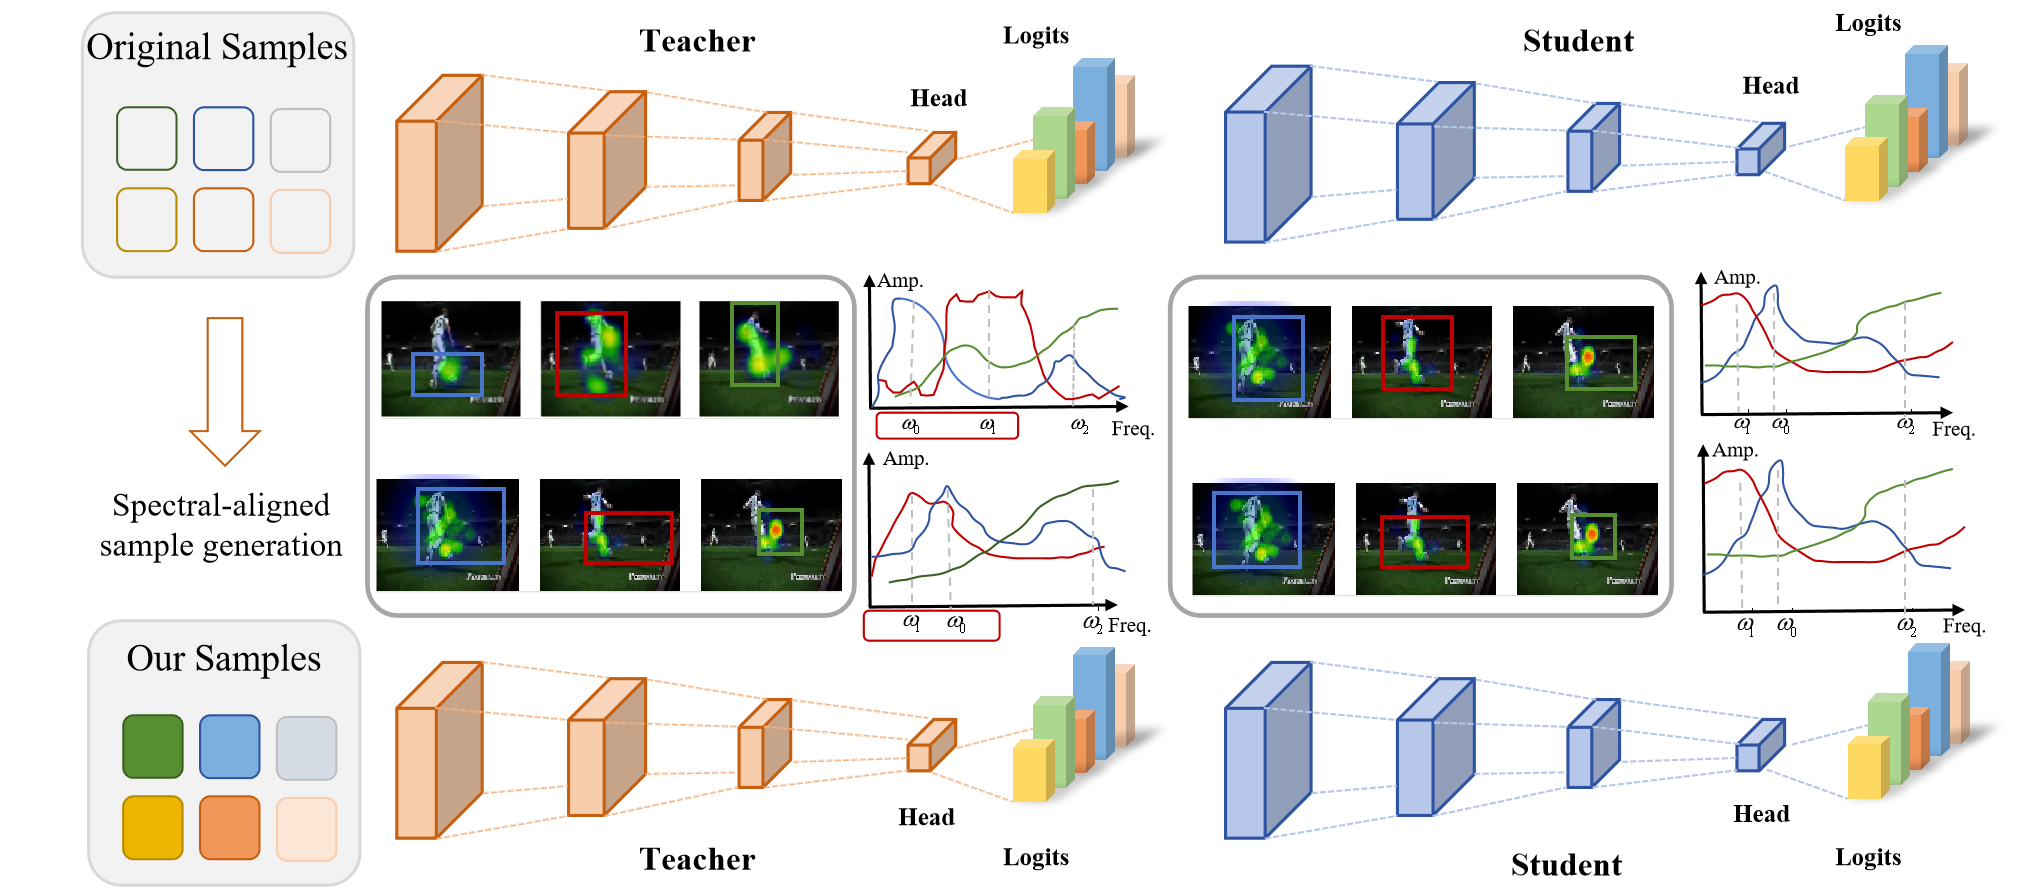
\includegraphics[width=1\linewidth]{pic/Motivation.png}
	\caption{Our Motivation}
	\label{Motivation}
\end{figure}


本论文的主要贡献包括: 

1)首次从样本生成的角度研究知识蒸馏中的特征对齐问题，通过主动调整输入数据分布来更高效地促进知识迁移。


2）在频域采用高斯掩码机制，根据中心频率差异自适应保留显著特征用于损失计算，并构建类别梯度库为样本更新提供指导，同时提出利用动态通道中心频率指导特征对齐过程，同时通过动态样本梯度建模类间相似性关系以指导蒸馏过程中的输出对齐。


总体而言，本文提出了一种面向动作识别任务的自适应样本生成与通道级动态知识蒸馏方法（ASCD）框架，在三个视频基准数据集（UCF101\cite{soomro-arxiv2012-ucf101}、Kinetics-400\cite{kay-arXiv2017-kinetics}、Something-Something V2\cite{goyal-iccv2017-sthsth}）和两个图像数据集（CIFAR-100\cite{wah-2011-cifar}、ImageNet\cite{krizhevsky-nips2012-imagenet}）上的大量实验验证了方法的有效性。


\section{Related Work}
在计算机视觉领域，视频动作识别与知识蒸馏作为两个重要的研究方向，近年来得到了广泛关注。视频动作识别技术主要通过对视频序列进行时空建模来实现对人类行为的理解与分类，其在智能监控、人机交互等领域具有重要应用价值。随着深度学习技术的快速发展，基于卷积神经网络（CNN）和循环神经网络（RNN）的方法在该领域取得了显著进展，特别是SlowFast\cite{feichtenhofer-iccv2019-slowfast}、TPN\cite{yang-cvpr2020-temporal}以及Video SwinTransformer\cite{liu-cvpr2022-video}等先进模型展现了卓越的性能。然而，这些高性能模型往往伴随着较高的计算复杂度，限制了其在资源受限场景下的应用。知识蒸馏作为一种高效的模型压缩技术，通过将复杂教师模型中的知识迁移到轻量级学生模型中，能够在保持模型性能的同时显著降低计算开销，该技术已在多种计算机视觉任务中得到成功应用。针对视频动作识别任务中的模型效率问题，本文从动作识别模型设计与知识蒸馏技术两个维度出发，系统性地回顾和分析了相关研究的最新进展与发展趋势。

\subsection{Knowledge Distillation}
知识蒸馏（Knowledge Distillation）作为模型压缩的最经典方法，主要通过将更大规模网络（教师模型）在训练数据上捕获的模式或规律迁移到较小规模网络（学生模型）得到轻量化模型，从而实现学习任务在资源受限下的快速推理，实现模型压缩，根据迁移的方法不同，知识蒸馏可以分为基于响应（Response）、基于特征（Feature）两种知识蒸馏方法。

\textbf{基于响应的蒸馏方法:}
基于响应的蒸馏直接利用教师模型的输出作为监督信号，指导学生模型的学习，教师模型输出的“软标记”（Soft Labels），包含类别间的概率分布信息，能够提供比硬标记更丰富的监督信号，帮助学生模型更好地学习类别间的相似性和决策边界；最早Hinton等人\cite{geoffrey-arxiv2015-kd}对教师模型的Logits进行软化得到软标记，使其能够向学生模型传递更多信息，此方法通过对教师 Logits 中显式信息的拆解来辅助学生模型学习，但由于教师与学生模型之间的决策机制存在差异，教师 Logits 所体现的类间关系未必适用于学生模型。针对这一问题，现有的工作往往通过调整蒸馏温度达到Logits的适配，Li 等人 \cite{li-aaai2023-ctkd} 提出根据学生模型的学习阶段动态调整蒸馏温度，称为“课程温度（Curriculum Temperature）”，以缩小教师与学生 Logits 之间的差异。其核心观点是，相较于静态设定，随训练进度调整温度系数能够更有效地服务于学生模型的学习过程，然而，在实践中，这类方法往往面临温度调节难以稳定收敛的问题，限制了其实际应用效果；在此基础上，Sun 等人 \cite{sun-cvpr2024-lskd} 推导出在教师与学生共享蒸馏温度的情形下，二者 Logits 值域被强行绑定，影响蒸馏效果，为此，提出一种 Logits 标准化方法，通过设置温度为 Logits 的加权标准差，以解决值域不匹配问题并提升知识迁移效率，然而此方法主要关注数值尺度上的归一化处理，未充分考虑 Logits 内部结构所蕴含的语义或类别间关系信息，因而在复杂任务或高度非对称的师生结构下，可能无法充分挖掘教师模型的知识潜力。

另一个方向是将Logit进行特定的分解，使其适配学生模型，Yang\cite{Yang-iccv2023-unifiedkd}将传统知识蒸馏（KD）损失分解为归一化 KD（NKD）损失，即对非目标类的教师与学生模型的Logits进行标准化后进行对齐；与之类似，Wu等人\cite{wu-eccv2022-tinyvit}对教师与学生模型的输出进行稀疏化，仅保留最重要的部分Logits输出，大大节省了在训练期间生成教师软标记的内存成本和计算开销。此类方法，通过拆解教师模型的Logits本身蕴含的显式信息，指导学生模型训练，但教师与学生模型的决策机制差异巨大，教师模型Logits提供的类间关系，往往并不适用学生模型。因此，Peng 等人 \cite{peng-icml2024-auxkd} 通过引入辅助变量重构教师模型的输出 Logits，旨在最大化师生特征间的互信息，并使学生模型的输出逼近教师模型的预定义分布。然而，该方法仅探索了一种辅助变量的实现形式与参数化方式，依赖较强的先验假设，因而在实际应用中往往难以达到最优效果。


基于响应的蒸馏方法自从提出以来，此蒸馏损失通常会作为其他蒸馏方法损失的一部分，然而在应用于目标定位、动作检测等复杂视频任务中时，仅从模型响应的角度，教师模型往往难以传递足够多的知识指导学生模型，导致蒸馏效率低下。



\textbf{基于中间特征的蒸馏方法:}
	基于特征的蒸馏方法，教师模型的一层或多层的中间层特征被用来传递知识，学生模型通过让输出的中间层特征尽可能接近教师模型，进而学习教师模型中的知识。通过捕捉教师模型在特征提取过程中的高阶语义信息，使学生模型更好地模仿教师模型的特征表示能力；早期，Han等人\cite{han-nips2015-learning}提出的FitNets将教师模型中指定一层的特征作为学习对象，通过1$\times$1卷积对齐通道数，计算其与学生模型相应层输出的L2距离，达到学生模型向教师模型学习的目的。自 FitNets 提出以来，大多数研究都致力于简化教师模型的中间特征表示，以便更好地与学生模型进行匹配。最近，Wang等人\cite{wang-aaai2024-gkd}利用条件变分自动编码器（CVAE）通过学习特征图和注意力图之间的对应关系，有效地重建特征语义，完成教师模型对学生模型特征语义的对齐，然而此方法需要训练额外的自编码器，引入了额外参数，增大了训练开销，且对所有学生模型采用同一个自编码器结构，缺乏针对不同学生架构的自适应调节能力；针对这一问题，	Liu等人\cite{liu-iclr2023-fkd}提出功能一致特征蒸馏，用来比较特征在“功能（Function）”上的差异，以弥补距离仅仅考虑“外表（Appearance）”上的差异这一不足，认为相较于学生模型与教师模型中间层特征在数值上接近，模型后续网络输入同样的中间层特征能够产生一致的输出更重要，本质上通过此方法间接生成教师与学生模型混合的助教网络,沿着这一思路，Wang等人\cite{wang-cvpr2024-crosskd}将学生检测头的中间特征传递给教师检测头,由此产生的Cross-Head预测与教师的预测进行对齐，使学生平衡了来自真实标记和教师预测的矛盾的监督信号，从而大大提高了蒸馏效率，此类方法的教师与学生模型特征交换位置的确定均作为超参人为设置，缺乏可解释性;少量工作从教师与学生模型输入差异的角度出发进行知识的适配，Guo等人\cite{guo-tpami2024-pixelkd}认为教师模型要求的高分辨率图像与学生模型要求输入的低分辨率图像会进一步加剧蒸馏过程中的教师与学生模型间知识的GAP，因此，利用特征预处理将CNN和ViT中的空间特征转换为相同的形式，使得教师模型向学生模型传递更适配的知识，然而所提出的特征转换方法引入大量额外参数，且构造缺乏可解释性;类似的，Li等人\cite{li-acmmm2025-slakd}首次指出不同训练样本之间可蒸馏的知识是不同的，每轮仅选取少量高蒸馏贡献度的训练样本参与训练，大大降低了训练开销，然而，这些高贡献样本始终受限于原始训练集本身的分布与多样性，无法引入新的语义或结构信息，难以突破原有数据所带来的信息瓶颈，限制了蒸馏过程对更丰富知识的挖掘与泛化能力的提升。
	
	与传统空间层面上的蒸馏方案不同，近年来也有少数工作专注于通道级蒸馏，Wang等人\cite{wang-nips2020-fusion}首次提出每个通道中包含的信息是通用的，甚至可以在不同的模态之间共享，为后续通道级蒸馏的发展提供坚实的基础，在此基础上，Shu等人\cite{shu-iccv2021-channelkd}通过 softmax 将通道特征转换为分布，以最小化教师和学生之间通道特征的差异；与之类似Tao等人\cite{tao-aaai2025-channelkd}通过通道注意力为每个通道设置蒸馏强度（attention score），然而此方法每次训练需要对每个通道单独计算通道注意力，计算量较高，且当样本数受限时训练效果较差；此类通道级蒸馏方法认为空间域和通道域之间存在着很强的相关性，即显著通道往往在空间域中包含重要的对象区域，然而教师模型决策逻辑，它并非显式存在于教师模型的中间特征中，而是体现为对特定频率、方向响应规律，直接通过 softmax 或通道注意力往往难以准确刻画这种隐式知识。
	
	基于中间特征的蒸馏方法，往往需要构造额外的辅助结构实现中间特征层维度的对齐。相较于基于响应的蒸馏方法，时间复杂度较高，泛用性较差，同时，随着Transformer\cite{vaswani-nips2017-attention}、Mamba\cite{gu-arxiv2023-mamba}等越来越多的网络结构提出，异构网络的蒸馏难度正在不断增加，额外的辅助结构不可避免的会越发复杂，待训练的参数量呈指数增加，需要依靠大量训练数据进行蒸馏，才能得到令人满意的效果。
\subsection{Dataset Distillation}
数据集蒸馏（Dataset Distillation）旨在通过合成少量高信息密度的样本来替代原始大规模训练集，从而在显著降低计算与存储成本的同时保持模型性能。早期方法如Wang等人\cite{wang-iclr2019-dataset}通过将网络权重表示为合成数据的可微函数，实现了从“优化权重”到“优化数据”的范式转变；随后，Zhao等人\cite{zhao-iclr2021-dcwgm}提出基于梯度匹配（Gradient Matching）的框架，使合成样本在训练中能产生与真实数据一致的梯度信号；类似的Cazenavette等人\cite{cazenavette-cvpr2022-ddmtt}进一步提出轨迹匹配（Trajectory Matching）方法，通过最小化合成与真实训练过程间的参数轨迹差距，实现对训练动态的精确复现，无论是基于梯度的数据集蒸馏还是基于轨迹的数据集蒸馏，均依赖于特定模型和任务，合成数据的迁移性较差，且对不同网络结构往往需重新优化，在每次优化中计算并存储大量梯度、轨迹信息，当模型或数据规模较大时额外开销较大。近年来，研究重心逐渐转向更具结构感知的优化目标，Cui等人\cite{cui-cvpr2025-optical}利用最优传输理论提出OPTICAL框架，通过动态分配真实样本对合成样本的贡献，实现细粒度的几何结构保持，然而最优传输距离的计算依赖于样本间的显式配对关系，对样本数量和分布平衡性较为敏感，可能导致蒸馏样本的语义多样性不足；最新的NCFM方法\cite{wang-cvpr2025-ncfm}通过引入基于神经特征函数的对抗式极小极大优化框架，自适应地学习分布差异度量，在特征空间中同时对齐幅度与相位信息，兼顾真实性与多样性，但这种对抗优化过程收敛性较差，在训练早期容易出现梯度不稳定问题。同时，此方法依赖于高维特征分布的神经近似，可解释性较弱，且在跨任务迁移时对特征空间变化的适应性有限。

视频数据集蒸馏旨在在保持时序语义一致性的前提下，将大规模视频数据压缩为少量可用于训练的合成样本，从而显著降低视频模型的训练与存储成本。与图像蒸馏相比，视频蒸馏需要同时建模空间结构与时间动态，在帧间冗余、时序连贯性、计算复杂度等方面面临更严峻的挑战。早期方法多将视频简化为帧级集合进行静态蒸馏，忽略了跨帧的运动与动态信息，导致生成样本缺乏时序一致性与动作可辨性。为解决这一问题，Wang等人\cite{wang-cvpr2024-vdsd}提出VDSD（Video Dataset Distillation via Static-Dynamic Memory），通过构建“静态记忆”与“动态记忆”双分支机制，将视频分解为静态关键帧与可学习运动补偿块，在保留空间语义的同时重建时序动态，实现了高效且稳定的视频蒸馏，然而此方法虽然有效缓解了帧间冗余问题，但其静态与动态特征的解耦仍较为粗糙，在复杂动作或长时依赖场景中，静态关键帧难以充分表达全局语义，而动态补偿块又难以捕捉跨帧的细粒度运动变化。进一步地，Zhao等人\cite{zhao-arxiv2024-idtd}提出IDTD（Inter-and Intra-sample Temporal Distillation），通过联合优化样本内帧间冗余与样本间结构相似性，构建时空一致的紧凑视频表示，有效保留动作语义并减少冗余帧信息，然而此方法虽然在样本内外冗余建模上实现了统一优化，但其优化目标主要集中于帧间结构相似性，缺乏显式的语义层对齐约束，可能导致生成的视频在视觉上时序平滑但语义辨识度不足。

现有视频数据集蒸馏方法，静态与动态信息的解耦仍不充分，现有方法通常依赖显式的静态-动态分支结构刻画时序星系，但这类分离机制难以精确捕捉复杂动作中的时空交互，导致生成样本在快速运动或长时依赖场景中表现不稳定，且计算与内存成本依然较高，尤其是在蒸馏高分辨率或长序列视频时，时空梯度匹配和特征对齐的复杂度呈指数增长。

。

\subsection{Action Recognition}
动作识别（Action Recognition）是一项重要的计算机视觉任务，旨在通过分析视频帧中的空间和时间信息识别视频中包含的单一动作类型，如“跑步”、“跳跃”等，在智能监控、医疗健康、智能家居和自动驾驶等领域有广泛应用。近年来，随着深度神经网络（Deep Neural Networks）不断发展\cite{krizhevsky-nips2012-imagenet}，过去以单一卷积神经网络为代表的模型逐步转变为基于转换器（Transformer）\cite{vaswani-nips2017-attention}或多网络结构融合的模型。不同于目标检测（Object Detection），动作识别模型不仅刻画目标的空间依赖关系，还要反映目标的时序动态特性。例如，通常考虑目标的运动轨迹、动作的连贯性、动作的持续时长等时序信息，以更好地理解和识别特定动作或行为。

在早期的视频动作识别方法中，建模时序信息主要分为两大类：基于光流的方法和基于 3D 卷积的方法。光流 \cite{horn-ai1981-determining} 是一种有效的运动表示，能够描述由于观察者与场景之间的相对运动而引起的图像中物体、表面和边缘的运动模式。Simon 等人 \cite{simon-nips2014-twostream}，认为运动信息在视频动作识别中至关重要，且难以通过常规卷积网络直接学习到。因此，他们首次提出了双流网络（Two-Stream Network），分别建模空间流和时间流：空间流以原始视频帧为输入，用于提取外观信息；时间流则以堆叠的光流图像为输入，用于捕捉帧间的短时运动信息。最终通过对两个分支的预测结果进行平均融合，得到最终的动作识别结果。尽管双流网络有效地建模了短期时序信息，但由于其仅关注局部帧间的运动，难以捕获长时间跨度的动态依赖。为了解决这一问题，Wang 等人 \cite{wang-eccv2016-action} 提出了时间段网络（Temporal Segment Network, TSN），该方法通过将视频划分为若干个时间段，从每个段中采样片段输入网络，并对各段的预测结果进行全局聚合，从而实现视频级别的动作识别。该策略在保留长时序信息的同时，有效降低了处理长视频序列所需的计算成本。

由于光流提取过程计算量大、存储要求高，不适合大规模训练或实时部署，理解视频的另一种简单方法是将其视为具有两个空间维度和一个时间维度的 3D 张量。Ji等人\cite{ji-tpami2012-3d}首次使用 3D卷积进行动作识别。后续提出的C3D\cite{tran-cvpr2015-learning}、I3D\cite{carreira-cvpr2017-kinetics}均在此基础上不断加深网络结构，并开始使用成熟的图像分类架构应用于3D卷积，Feichtenhofer等人开始将3D卷积引入双流架构，但它与传统双流网络不同这两条路径旨在建模不同的时间速度，而不是空间和时间建模，提出的Slowfast\cite{feichtenhofer-iccv2019-slowfast}是一种具有慢速路径和快速路径的高效网络，慢速路径以低帧速率运行以捕获详细的语义信息，而快速路径以高时间分辨率运行以捕获快速变化的运动，然而Slowfast双分支网络，由于固定了快慢路径中3D卷积核大小，仍然不能覆盖各种动作节奏。

自Transformer在图像领域取得巨大成功，有不少研究者将Transformer应用于视频动作识别中\cite{dosovitskiy-iclr2021-transformers}\cite{arnab-iccv2021-vivit}\cite{liu-cvpr2022-video}\cite{yan-cvpr2022-multiview}，VTN\cite{neimark-cvpr2021-video}在预先训练的 ViT 之上添加一个时间注意力编码器，借助滑动窗口机制，代替传统3D卷积实现冗长的时间序列处理,在VTN架构的基础上为了进一步提高建模效率，ViViT \cite{arnab-iccv2021-vivit}精简视频输入的token数，在空间和时间维度上分别对Transformer编码器各组件进行四种分解设计;MViT\cite{fan-cvpr2021-multiscale}逐步增加信道维度，同时降低整个网络的时空分辨率（即序列长度），通过集中时空建模的注意力来减少计算量，这些模型均使用大规模 ImageNet-21K\cite{ridnik-nips2021-imagenet}JFT-300M\cite{sun-iccv2017-revisit}、JFT-3B\cite{zhai-cvpr2022-scaling}预训练模型提出不同的空间和时间注意力设计新模型，改进模型对视频识别时空建模能力，为了解决现有Transformer架构对大规模图像数据预训练模型的依赖问题，Tong等人\cite{tong-nips2022-videomae}提出的VideoMAE通过时序下采样来减少时空冗余性和数据维度，并采用管道式掩码策略在视频序列中遮蔽相同位置的视觉像素块进行重构，这种设计不仅加速了预训练过程，还显著提升了模型的表征能力，然而，VideoMAE的低级特征重建收敛极为困难，同时低级特征的重建可能不总能有效捕捉高级语义信息，且由于全局自注意力，处理屏蔽和未屏蔽token的额外解码器会导致较高的内存成本，针对这些问题，Li 等人 \cite{li-cvpr2023-unmasked} 通过掩码处理低语义 token 来减少训练开销，并仅用线性映射层对齐未掩码token，从而降低了解码器的运算量，此外，还引入了以原始图像为输入的预训练教师模型来指导重构过程；最近，Wu等人\cite{wu-iccv2023-temporal}选取固定的相邻帧作为每个视频帧的上下文帧，并在空间维度上应用算术操作，以捕捉时序信息，后续利用特征提取器提取这些时间线索的空间表示，并通过空间转换将结果与原始特征残差连接，最终为视频识别提供有效的时间信息，然而，在空间维度的算术操作（加减乘除）捕捉时序信息的方式缺乏可解释性，同时，固定的上下文范围可能无法充分捕捉视频中的关键时间信息。

早期无论是结合了空间流人\cite{ji-tpami2012-3d}（处理单帧图像）和时间流（处理光流图像）\cite{simon-nips2014-twostream}的双流网络还是在视频的时空维度上进行卷积操作捕捉时空信息的3D卷积网络，一旦尝试刻画长期时序依赖，以及高分辨率的视频样本时，计算量将呈指数级增长；随着Transformer应用于视频动作识别中，利用自注意力机制捕捉长距离依赖关系，虽然时序关系建模效率大幅提升，但Transformer架构\cite{dosovitskiy-iclr2021-transformers}的网络通常具有大量的参数，不可避免地增大了计算成本和训练难度，不仅延长了推理时间，同时也加大了在计算资源受限的边缘和端侧设备的部署压力，如何实现高效的计算与准确的识别已成为实际部署中的关键问题

关于动作识别模型的知识蒸馏最新的工作较少，大多数早期的工作\cite{crasto-cvpr2019-mars}\cite{stroud-wacv2020-d3d}\cite{thoker-icip2019-crosskd}，主要关注于跨模式（光流和RGB）蒸馏策略，旨在通过实现光流（教师模型）实现向 RGB 流（学生模型）的迁移来增强模型性能，无法应用于最新基于Transformer的大规模动作识别模型；针对动作识别任务的中间特征语义信息，Wang等人\cite{wang-aaai2024-gkd}提出了基于生成模型的特征知识蒸馏框架，对教师与学生模型的中间特征通过条件变分自编码器（CVAE，Conditional Variational Autoencoder）提炼基于注意力的特征信息，然而此方法需要训练额外的自编码器，引入了额外参数，增大了训练开销。现有对于动作识别模型的知识蒸馏的工作，缺少针对最新模型结构（Transformer）的蒸馏方法，同时，现有的蒸馏方法忽略了时空信息在视频样本中的重要作用，针对上述局限，Li 等人\cite{li-acmmm2025-slakd} 最近提出了一种样本级自适应知识蒸馏方法——SAKD（Sample-level Adaptive Knowledge Distillation）。该方法在训练过程中通过对视频帧在时间维度上进行随机打乱Shuffle或Mask，根据教师模型与学生模型之间蒸馏损失的变化，动态评估各个视频样本的时序依赖程度；然而，该方法较为依赖超参数的设置。当 Mask 或 Shuffle 的比例过高时，可能会遮挡原始视频片段中的关键动作，导致时序信息严重丢失。此时，不仅无法实现预期的数据增强效果，反而会使学生模型难以有效捕捉视频样本中的关键动作特征，从而影响蒸馏效果。

\section{模型方法}
\subsection{Problem Definition and Preliminary}

知识蒸馏作为模型压缩的经典方法，主要利用更大规模网络（教师模型$\mathcal{T}$）的知识迁移到较小规模网络（学生模型 $\mathcal{S}$）得到轻量化模型，从而实现学习任务在资源受限下的快速推理，达到模型压缩的目的。给定一个视频数据集，将其分为训练集 $\mathcal{D}_{\text{train}} = \{\mathcal{V}_i, y_i\}_{i=1}^N$
和测试集 $D_{\text{test}} = \{\mathcal{V'}_i, y'_i\}_{i=1}^{N'}$其中 $\mathcal{V}$ 是视频样本，$y \in \mathbb{R}$ 是来自 $K$ 个类别的动作标记。在每个视频上进行随机采样以获得 $T$ 帧。对于第 $i$ 个视频片段，其高度为$H$、宽度为 $W$ 的 RGB 帧堆叠为一个张量 $\textbf{X}_i \in \mathbb{R}^{3 \times T \times H \times W}.$
因此，训练集为 $\textbf{X} = \{\textbf{X}_i, y_i\}_{i=1}^N,	$用于学生模型学习；测试集为$\textbf{X}' = \{\textbf{X}'_i, y'_i\}_{i'=1}^{N'}$	用于推断。

在训练过程中，训练集中的视频片段 $\textbf{X}$被同时输入到教师模型 $\mathcal{T}$ 和学生模型 $\mathcal{S}$。这些模型的backbone采用常用的动作识别骨干网络如Slowfast\cite{feichtenhofer-iccv2019-slowfast}，生成教师模型中间特征集合${{\cal F}^\mathcal{T}} = \left\{ {{\textbf{F}}_{j}^\mathcal{T}\left| {0 < j \le L} \right.} \right\}$和学生模型中间特征集合${{\cal F}^\mathcal{S}} = \left\{ {{\textbf{F}}_{j}^\mathcal{S}\left| {0 < j \le L} \right.} \right\}$，其中${\textbf{F}}_j^\mathcal{T} \in {^{t_j^\mathcal{T} \times w_j^\mathcal{T} \times h_j^\mathcal{T} \times c_j^\mathcal{T}}}$，${\textbf{F}}_j^\mathcal{S} \in {^{t_j^\mathcal{S} \times w_j^\mathcal{S} \times h_j^\mathcal{S} \times c_j^\mathcal{S}}}$， $t,c, h, w$ 分别表示时间、通道、高度和宽度维度，$n$为从Backbone中提取的中间特征个数。

对于基于 Logit 的知识蒸馏，蒸馏损失通过最小化教师和学生输出概率之间的差异来实现，即：
\begin{equation}
\mathcal{L}_{kd}^{logit} = \frac{1}{N} \sum_{i=1}^N \tau^2 \text{KL}(\sigma(q^\mathcal{T}_i / \tau), \sigma(q^\mathcal{S}_i / \tau)),
\label{logit}
\end{equation}
其中 $\text{KL}(\cdot)$ 是 Kullback-Leibler 散度，$\{q^\mathcal{T}, q^\mathcal{S}\}$ 分别是教师和学生的 logits，$\sigma(\cdot)$ 是 softmax 函数，$\tau$（设置为 4）是用于调整两个概率分布平滑度的温度系数。

对各层教师和学生模型的特征图 $\textbf{F}_j^\mathcal{S}$的维度通过一个映射函数$f(\cdot)$（例如 1$\times$1 卷积或自编码器）进行对齐。对于基于特征的知识蒸馏（KD），蒸馏损失通过最小化教师和学生特征之间的差异，使学生模仿教师，即：
\begin{equation}
\mathcal{L}_{kd}^{fea} = \frac{1}{N} \sum_{i=1}^N \sum_{l=1}^L\| f(\textbf{F}^T_{i,l}) - f(\textbf{F}^S_{i,l}) \|_2^2,
\end{equation}
其中 $\|\cdot\|_2$ 表示 $\ell_2$-范数,$\textbf{F}_{i,j}$表示第$i$个样本第$j$层中间特征。

特别的，通道蒸馏在传统基于中间特征蒸馏的基础上，引入通道权重系数 $\textbf{W}_{i,j,k}$，逐通道加权对齐，用于调整每个通道蒸馏误差对总损失的贡献。通道加权蒸馏损失定义如下：
\begin{equation}
\mathcal{L}_{kd}^{channel} = \frac{1}{N} \sum_{i=1}^{N} \sum_{l=1}^{L} \sum_{c=1}^{C_j} \textbf{W}_{i,l,c} \left\| \textbf{F}^{\mathcal{T}}_{i,l,c} - \textbf{F}^{\mathcal{S}}_{i,l,C} \right\|_2^2
\end{equation}
其中 $\textbf{W}_{i,l,c} \in \mathbb{R}_{\ge 0}$ 表示第 $i$ 个样本、第 $l$ 层、第 $c$ 个通道的重要性权重，往往通过教师模型的通道响应强度、注意力机制或统计信息自动学习得到。



动作识别模型的基础损失采用交叉熵Cross-Entropy (CE)损失：
\begin{equation}
\mathcal{L}_{\text{ce}} = -\frac{1}{N} \sum_{i=1}^N \textbf{y}_i \log \textbf{q}^\mathcal{S}_i.
\label{ce_loss}
\end{equation}
	\subsection{符号定义}
\label{define}
\begin{table}[!htb]
	\centering
	\caption{本文主要符号及其含义说明}
	\small 
	\begin{tabular}{lll}
		\toprule[0.75pt]
		符号             & 维度                                                                               & 符号含义                                  \\ \hline
		$\mathcal{S}$    &                                                                                   & 学生模型                                  \\
		
		$\mathcal{T}$    &                                                                                   & 教师模型                  \\
		$\mathcal{D}_{train}$              &                                                                                   & 完整训练集                 \\
		$\hat{\mathcal{D}}_{train}$              &                                                                                   & 适合进行蒸馏训练集                 \\
		$\mathcal{D}_{test}$              &                                                                                   & 完整测试集                 \\
		$N$              &                                                                                  & $D_{train}$ 中包含的训练样本数             \\
		$N'$          &                                                                                   & $D'_{test}$ 包含的测试集样本数             \\
		$K$          &                                                                                   & 数据集中动作类别数       \\
		
		$\textbf{X}_i$  &            $\mathbb{R}^{3 \times T \times H \times W}$                                                                 & $\mathcal{D}_{train}$中第$i$个视频片段               \\
		$\hat{\textbf{X}}_i$&            $\mathbb{R}^{3 \times T \times H \times W}$                                                                 &第$i$个优化后的高效蒸馏的视频样本片段\\
		$\textbf{X}'_{i'}$  &            $\mathbb{R}^{3 \times T \times H \times W}$                                                                 & $\mathcal{D}_{test}$中第$i'$个视频片段                 \\
		$\mathcal{V}_i$&  &训练集$\mathcal{D}_{train}$第$i$个视频\\
		$\mathcal{V}'_{i'}$&  &测试集$\mathcal{D}_{test}$第$i'$个视频\\
		$\omega^\mathcal{T}_{l}$&  $\mathbb{R}^{1 \times C_l^\mathcal{T} }$ & 教师模型第$l$层中间特征的各通道中心频率\\
		$\omega^\mathcal{S}_{l}$&  $\mathbb{R}^{1 \times C_l^\mathcal{S} }$ & 学生模型第$l$层中间特征的各通道中心频率\\
		$\textbf{b}^\mathcal{T}_{l}$&  $\mathbb{R}^{1 \times C_l^\mathcal{T} }$ & 教师模型第$l$层中间特征的各通道核心频率带宽\\
		$\textbf{b}^\mathcal{S}_{l}$&  $\mathbb{R}^{1 \times C_l^\mathcal{S} }$ & 学生模型第$l$层中间特征的各通道核心频率带宽\\
		$\mathcal{G}$&  &类梯度方向Memory Bank \\
		$\textbf{F}_l^\mathcal{T}$&$\mathbb{R}^{C_l^\mathcal{T} \times T_l^\mathcal{T} \times  H_l^\mathcal{T}\times  W_l^\mathcal{T}}$&教师模型第$l$层中间特征\\
		$\textbf{F}_l^\mathcal{S}$&$\mathbb{R}^{C_l^\mathcal{S} \times T_l^\mathcal{S} \times  H_l^\mathcal{S}\times  W_l^\mathcal{S}}$&学生模型第$l$层中间特征\\
		$\hat{\textbf{F}}_l^\mathcal{S}$&$\mathbb{R}^{C_l^\mathcal{T} \times T_l^\mathcal{T} \times  H_l^\mathcal{T}\times  W_l^\mathcal{T}}$&学生模型与教师模型对齐后第$l$层中间特征\\
		$\dot{\textbf{F}}_l^\mathcal{T}$&$\mathbb{R}^{C_l^\mathcal{T} \times T_l^\mathcal{T} \times H_l^\mathcal{T} \times W_l^\mathcal{T}}$&高效蒸馏的视频样本输入教师模型后第$l$层的中间特征\\	
		$\bar{\textbf{F}}_l^\mathcal{T}$&$\mathbb{R}^{C_l^\mathcal{T} \times T_l^\mathcal{T} \times H_l^\mathcal{T} \times W_l^\mathcal{T}}$&教师模型第$l$层特征频域掩码后经过傅里叶逆变换后结果\\
		$\bar{\textbf{F}}_l^\mathcal{S}$&$\mathbb{R}^{C_l^\mathcal{T} \times T_l^\mathcal{T} \times H_l^\mathcal{T} \times W_l^\mathcal{T}}$&对齐后学生模型第$l$层特征频域掩码后经过傅里叶逆变换后结果\\
		$\text{Mask}_{l,c}^\mathcal{T}(\boldsymbol{\omega})$&$\mathbb{R}^{C_l^\mathcal{T} \times T_l^\mathcal{T} \times H_l^\mathcal{T} \times W_l^\mathcal{T}}$&表示教师模型第 $l$ 层第 $c$ 通道在频率点 $\boldsymbol{\omega}$ 处的高斯滤波权重\\
		$\tilde{\textbf{F}}_{l,c}^\mathcal{T}$&$\mathbb{R}^{C_l^\mathcal{T} \times T_l^\mathcal{T} \times H_l^\mathcal{T} \times W_l^\mathcal{T}}$&对齐后教师模型第$l$层特征频域掩码后结果\\
		$\omega_{l,c}^\mathcal{T}$&&教师模型第$l$层$c$通道中心频率\\
		$\omega_{l,c}^\mathcal{S}$&&学生模型第$l$层$c$通道中心频率\\
		$q^{\mathcal{S}}_i$&&第$i$个训练样本输入学生模型得到logits\\
		$q^{\mathcal{T}}_i$&&第$i$个训练样本输入教师模型得到logits\\
		$L$&&蒸馏过程中选取的中间特征总层数\\
		$\tau$&$\tau\in[1,+\infty]$&蒸馏温度\\
		$\textbf{g}_{\text{epoch}}$&$\mathbb{R}^{3 \times T \times H \times W}$  &类梯度方向\\
		$\text{gain} $&&判断是否对样本进行更新的更新增益\\
		$\alpha$&&损失中通道级蒸馏损失的系数\\
		$\beta$&&损失中kd损失的系数\\
		$\gamma$&&损失中aux辅助损失的系数\\
		$\lambda$&&控制原始视频输入更新强度的超参\\
		$\eta $&&控制原始视频输入更新速率的超参\\
		\toprule[0.75pt]
	\end{tabular}
	\label{tab.param_def}
\end{table}

论文中出现的主要符号如表\ref{tab.param_def}所示。


\begin{figure}[h]
	\centering
	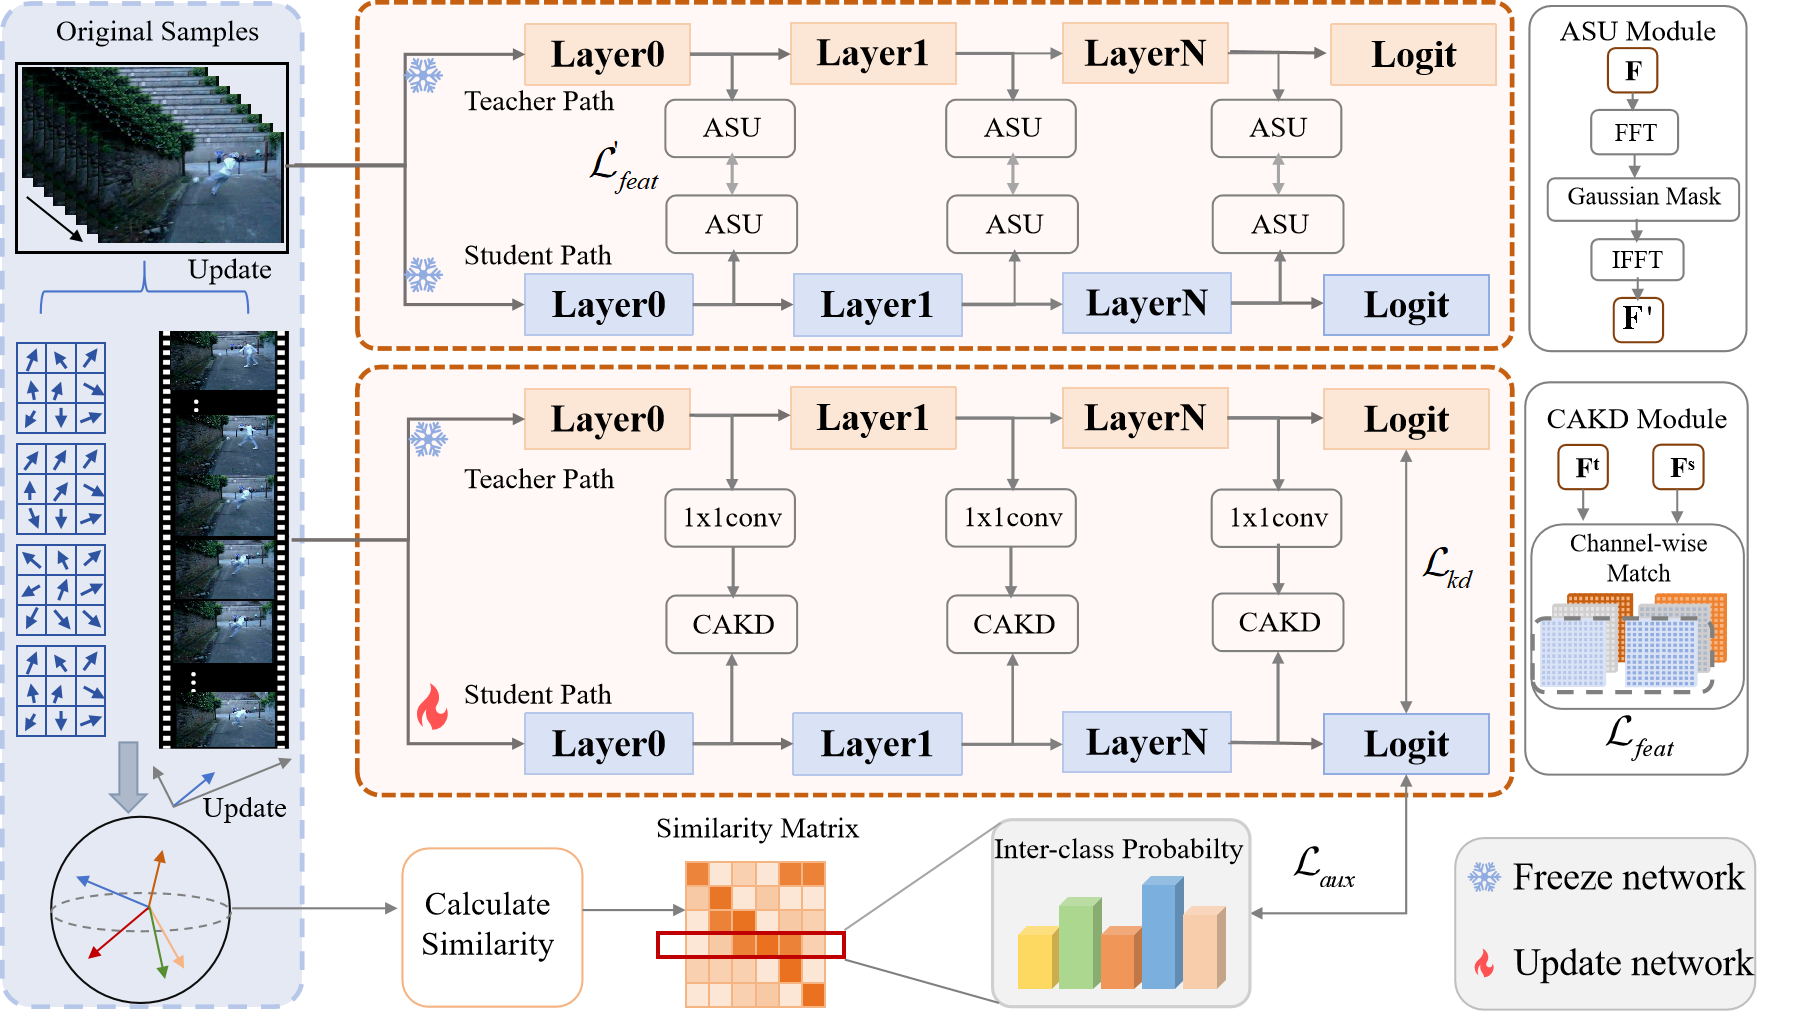
\includegraphics[width=1\linewidth]{pic/FrameWork.png}
	\caption{Our Method模型结构图}
	\label{Method}
\end{figure}
总体框架如图 \ref{Method} 所示，

\subsection{模型框架} 
频域自适应适配蒸馏方法主要包括蒸馏自适应样本生成模块以及通道级动态蒸馏模块组成。不同于以往基于原始训练数据进行蒸馏的范式，本方法在蒸馏前通过生成更适配蒸馏任务的训练样本，动态构建新的训练集 $\hat{\mathcal{D}}_{train}$，以提升蒸馏效果。


首先为教师模型与学生模型的蒸馏层初始化可学习的中心频率与频率带宽，并为每个类别构建对应的类梯度记忆库（Class-wise Gradient Memory Bank），将训练集$\mathcal{D}_{train}$输入蒸馏自适应样本生成模块，具体来说，将原始视频$\textbf{X}$ 分别输入教师与学生模型，提取中间特征后，通过频域掩码提取频率本征特征，以去除冗余干扰信息，后续将对齐教师与学生模型本征特征与中心频率作为优化目标，冻结教师与学生模型，通过优化原始训练样本更新类梯度记忆库中每类最优梯度方向，并据此生成更适合蒸馏任务的样本集 $\hat{\mathcal{D}}_{train}$ 。

后续将新的训练集$\hat{\mathcal{D}}_{train}$ 输入通道级自适应蒸馏模块中，将教师与学生模型的中间特征$\textbf{F}^\mathcal{T}$与$\textbf{F}_l^\mathcal{S}$通过1$\times$1卷积对齐形状后执行逐通道频率加权对齐，同时引入基于类间梯度相似性的隐式约束来调节学生模型输出$q^{\mathcal{S}}$，进一步提升蒸馏效果。为平衡训练效率与输入更新开销，引入累计Poly策略\cite{wu-tist2023-poly}，动态控制样本更新时机。该方法在保障特征判别性与模型对齐效率的同时，提升了视频蒸馏的稳定性与泛化能力。


\subsection{蒸馏自适应样本生成模块} 
现有的针对视频动作识别的蒸馏任务中，往往直接借用图像分类的蒸馏方法，忽略了视频具有重要的时序特征，使得训练出来的学生模型鲁棒性较差，效果易受超参、数据集影响；同时，传统知识蒸馏方案中教师模型向学生模型传递的知识受到原始数据的约束，这在很大程度上限制了教师模型知识的传递,最适合蒸馏任务的样本输入，有可能不存在于原始数据之中，其主要原因在于原始数据的分布有限，有可能无法全面覆盖教师模型所学习到的深层次隐式知识（即教师模型隐式决策逻辑，它并非显式存在于某个样本的标记或中间特征中，而是体现为对特定频率、方向响应规律）且输入样本独立教师模型之外，能保证教师模型从性能最优的教师模型向最优教师模型转变时，教师模型无需重新训练;此外，教师模型在不同层级的特征在频率分布上存在显著差异，尤其在视频动作识别任务中更为突出，视频中的动作本质上体现为时空频率结构的变化，例如周期性运动、高频瞬时行为或低频持续动作等。由于模型在不同层捕捉的特征频率分布相对固定且不同，尤其在视频建模中，运动信息往往集中在特定频率段，而在图像中高频对应像素值在短距离内剧烈波动（如边缘）等，低频对应图像中缓慢变化的区域，如大块颜色区域、背景等，部分图像如识别$Elephants$
时，低频轮廓（大耳朵、长鼻子）比皮肤纹理更重要，而某些图像例如$Beaver$、$Porcupine$这类动物，依赖于毛发纹理进行识别的动物，往往需要高频信息。

现有知识蒸馏方法通常采用固定输入（静态样本）进行特征或逻辑值的对齐，这限制了蒸馏性能——因为原始数据分布可能并非传递教师网络至学生网络知识的最佳载体。为此，我们设计了自适应样本生成（ASG）模块，通过梯度引导自适应生成样本，以优化师生网络间的特征对齐。该模块的技术动机源于两个方面：其一，不同网络层或同一层的不同通道可能捕获样本的不同特性（如低层视觉线索中的边缘信息与高层语义中的运动变化），因此我们实施跨层的通道级特征对齐；其二，视频或图像存在固有冗余，可通过频域进行降维处理。这促使我们将特征从空间域投影至频域，通过具有可学习中心频率的自适应高斯掩码，保留关键频率特征（如相关运动信号），同时抑制无关噪声（如相机抖动、光照变化）。具体实现如下



受最近一些数据集蒸馏的工作\cite{lei-tpami2024-survey}\cite{lee-icml2022-dataset}\cite{liu-nips2022-dataset}启发，针对上述问题，本文提出的蒸馏自适应样本生成模块,与传统数据集蒸馏方法直接利用原始训练数据进行蒸馏，缺乏针对蒸馏任务的样本优化过程不同，本文通过频域高斯掩码提取教师/学生模型中间特征特定频率的本征特征，即与当前学生与教师模型中间特征匹配度最高的频带特征，去除干扰性冗余信息，将教师与学生的本征特征对齐作为优化目标，冻结模型参数，通过优化原始样本输入以更新类梯度记忆库中各类别的代表性梯度方向。在此基础上，进一步反向优化训练样本，使其朝向更有利于蒸馏的方向分布，从而动态构建出更适配当前蒸馏任务的训练集 $\hat{\mathcal{D}}_{train}$，有效提升后续特征对齐与学生模型训练的效果。


具体来说，首先从原始数据集$\mathcal{D}_{train}$中取出训练样本$\textbf{X}_i \in \mathbb{R}^{3 \times T \times H \times W}$(其中$T$代表视频片段包含帧数,$H$和$W$分别表示视频帧的高和宽，$i\in [1,N]$,$N$ 为训练集中样本总数)分别输入教师模型$\mathcal{T}$与学生模型$\mathcal{S}$中，得到教师模型中间特征集${{\cal F}^\mathcal{T}} = \left\{ {{\textbf{F}}_{l}^\mathcal{T}\left| {0 < l \le L,} \right.{\textbf{F}}_l^\mathcal{T} \in {^{T_l^\mathcal{T} \times W_l^\mathcal{T} \times H_l^\mathcal{T}\times C_l^\mathcal{T}}}} \right\}$与学生模型中间特征集${{\cal F}^\mathcal{S}} = \left\{ {{\textbf{F}}_{l}^\mathcal{S}\left| {0 < l \le L,} \right.{\textbf{F}}_l^\mathcal{S} \in {^{T_l^\mathcal{S} \times W_l^\mathcal{S} \times H_l^\mathcal{S}\times C_l^\mathcal{S}}}} \right\}$,其中$\textbf{F}_{l}$代表教师/学生模型第$l$层中间特征，$T_l$、$W_l$、$H_l$、$C_l$分别表示第$l$层中间特征时间、宽、高、通道维度的大小，$l\in [1,L]$,将各层学生模型通过1$\times$1 $Conv_l$对齐教师与学生特征的$W_l$、$H_l$、$C_l$维度，通过线性插值函数$\mathcal{I}(\textbf{F}_l^\mathcal{S},T_l^\mathcal{T})$，将学生模型中间特征的时间维度$T_l^\mathcal{S} $变为$T_l^\mathcal{T}$,

%即以第$l$层为例：
%	\begin{equation}
%		\hat{\textbf{F}}_l^\mathcal{S}=\mathrm{Intpol}(Conv_l(\textbf{F}_l^\mathcal{S}),T_l^\mathcal{T}),
%		\label{Aug}
%	\end{equation}
%其中$\mathrm{Intpol}(.)$为时间维度的线性插值，

为增强时空建模能力，我们通过三维离散傅里叶变换将视频特征从空间域映射至频域。空间频率被分解为低频与高频分量：低频对应结构信息、平滑区域（微小变化）及语义内容（如墙面或物体主体），高频则呈现精细运动细节、边缘特征及噪声（如纹理、锐利轮廓）。同时，时域频率被分解为低频时序与高频时序分量：低频指示缓慢渐变或静态背景，高频则反映快速运动与剧烈变化。此外，离散傅里叶变换通过全局运算捕获长程依赖关系，并借助乘法实现快速处理。具体而言，第$l$层通道$c$的频率特征计算公式如下*(上标$\mathcal{S}$和$\mathcal{T}$在此忽略)：

\begin{equation}
\hat{\textbf{F}}_{l,c}(z,u,v)
=
\sum_{t,h,w=0}^{T_l-1,\,H_l-1,\,W_l-1}
\textbf{F}_{l,c}(t,h,w)\,
e^{-j 2\pi \left( \frac{z t}{T_l} + \frac{u h}{H_l} + \frac{v w}{W_l} \right)} ,
\label{eq:dft}
\end{equation}

在公式~\eqref{eq:dft} 中，对模型第 $l$ 层第 $c$ 个通道的特征图 $\textbf{F}_{l,c}^\mathcal{T} \in \mathbb{R}^{T_l^\mathcal{T} \times H_l^\mathcal{T} \times W_l^\mathcal{T}}$ 进行三维离散傅里叶变换，其变换结果表示为 $\hat{\textbf{F}}_{l,c}(z,u,v)$，其中$z = 0,1,\ldots T_l-1$ 、$h =  0,1,\ldots H_l-1$、$w =  0,1,\ldots W_l-1$分别代表时间维度、垂直空间维度、水平空间维度的离散位置索引,$j$代表虚数符号；

\textbf{高斯掩码}为了保留视频中语义上显著的运动模式，我们引入高斯掩码 Mask(·) 作为一种滤波器，其具有动态的中心频率 \((z_o, u_o, v_o)\) 和带宽 \(b_{l,c}\)，这些参数均可通过反向传播进行学习：
\begin{equation}
\text{Mask}_{l,c}(z, u, v) = e^{-\frac{(z - z_o)^2 + (u - u_o)^2 + (v - v_o)^2}{2b_{l,c}^2}}.
\label{eq:teacher-mask}
\end{equation}

高斯掩码围绕中心频率 \(\omega_{l,c} = (z_o, u_o, v_o)\)，保留了一段相关的频率带，即动作的基本频率及其直接谐波。这对应于视频中不同空间区域之间的连贯运动模式。

我们将高斯掩码应用于公式（eq:dft）中的逐通道频率特征，从而得到滤波特征，即
\begin{equation}
 \tilde{\textbf{F}}_{l,c}(z, u, v) = \hat{\textbf{F}}_{l,c}(z, u, v) \odot \text{Mask}_{l,c}(z, u, v), 
\label{eq:mask}
\end{equation}
这里，“\(\odot\)”表示元素级乘积。由于中心频率是动态学习的，因此该滤波器能够适应同一类别视频中不同的动作模式。它既能够保留快速动作（如拍手）的高频成分，也能够保持慢速动作（如站立）的低频成分。这就提供了一种自适应的时间平滑处理，以适应主要运动模式。

后续在频域进行$\mathrm{Mask}$后的滤波后的特征通过逆离散傅里叶变换（IDFT）被投影回空间域，即：

\begin{equation}
\tilde{\textbf{F}}_{l,c}^{-1}(t, h, w) = \frac{1}{N_f} \sum_{z,u,v=0}^{T_1-1,H_1-1,W_1-1} \tilde{\textbf{F}}_{l,c}(z, u, v) \cdot e^{j2\pi\left(\frac{zt}{T_1} + \frac{uh}{H_1} + \frac{vw}{W_1}\right)},
\label{eq:idft}
\end{equation}

其中，\(N_f = T \cdot H \cdot W\) 为频率分量的数量，用作归一化因子。保留其实部以构成增强特征 \(\{\overline{F}^{\mathcal{T}}_{l,c}, \overline{F}^{\mathcal{S}}_{l,c}\} \in \mathbb{R}^{T_l \times H_l \times W_l}\)。将教师与学生模型各层特征频域掩码后经过傅里叶逆变换后结果计算加权损失:

\begin{equation}
\mathcal{L}_{kd}^{fea} = \frac{1}{N} \sum_{i=1}^{N} \sum_{l=1}^{L} \sum_{c=1}^{C_l} \frac{\|\tilde{\textbf{F}}_{l,c}^{\mathcal{T}} - \tilde{\textbf{F}}_{l,c}^{\mathcal{S}}\|_2^2}{\|\omega_{l,c}^{\mathcal{T}} - \omega_{l,c}^{\mathcal{S}}\|_2^2 + \varepsilon}
\label{eq:align}
\end{equation}


其中 \(\varepsilon\)（设为 \(1\mathrm{e}{-6}\)）是一个平滑因子，用于避免分母为零。注意，在每一层都对中心频率 \(\omega_l\) 应用了层归一化。权重被设置为中心频率差异的倒数，作为对齐强度。由于输入样本在第一阶段已被更新，此时的对齐特征可能并非最优，尤其是当频率差异较大时。因此，我们鼓励在频率差异较小时进行逐通道特征对齐，而在频率差异较大时则抑制对齐。这是因为教师模型与学生模型之间相似的中心频率表明其特征已较好对齐。



%
%其中$\sum_{c=1}^{C_l^T} \frac{\left\| \bar{\textbf{F}}^{\mathcal{T}}_{i,l,c} - \bar{\textbf{F}}^{\mathcal{S}}_{i,l,c} \right\|_2^2}{\left\| \text{LN}(\omega_{l,c}^\mathcal{T})-\text{LN}(\omega_{l,c}^\mathcal{S}) \right\|_2^2+\epsilon}$是评判各层是否为最佳教师的重要指标，其值越大，该层特征越适合作为教师，向学生模型传递知识，当教师与学生的中间特征经过高斯掩码的特征，当第$i$个样本第$l$层教师特征$\sum_{c=1}^{C_l^T} \bar{\textbf{F}}^{\mathcal{T}}_{i,l,c}$与学生特征$\sum_{c=1}^{C_l^T} \bar{\textbf{F}}^{\mathcal{C}}_{i,l,c}$差异较大时，说明该层教师与学生模型特征差异较大，学生模型可以有更多知识可以学习，但若教师模型关注的中心频段与学生模型关注的中心频段差异过大，该式子的分母也会变大，即学生模型与教师模型的适配性变差。




\textbf{Memory Bank}
为了计算样本梯度，我们在当前 epoch 中使用已更新的样本，在通道维度上对公式\ref{eq:align} 中的加权特征损失进行优化。逐通道的梯度被拼接起来，形成样本梯度 \(\textbf{g}_{k}^{m} \in \mathbb{R}^{T \times H \times W \times C}\)，其中 \(m = 1, 2, \dots, M_k\) 表示类别 \(k\) 中的第 \(m\) 个样本（共 \(M_k\) 个样本）。同一类别中的所有样本共享该类别的梯度。随后，\(\textbf{g}_{k}^{m}\) 被用于以累积方式更新类别 \(k\) 的梯度，即


\begin{equation}
\textbf{g}^k \leftarrow \frac{\textbf{g}^k + \textbf{g}_m^k}{\|\textbf{g}^k + \textbf{g}_m^k\|_2} \cdot \min(\|\textbf{g}^k\|_2, \|\textbf{g}_m^k\|_2)
\label{eq:grad}
\end{equation}
其中 \(\textbf{g}^k\) 由 \(\textbf{g}_1^k\) 初始化。两个样本梯度之和经过归一化以确定梯度方向，而较小梯度的范数则作为权重，用于控制梯度更新的幅度。所有类别的梯度均按公式\ref{eq:grad} 计算，从而得到梯度集合 \(\mathcal{G} = \{\textbf{g}^1, \textbf{g}^2, \dots, \textbf{g}^K\}\)，即梯度库（gradient bank）。该梯度库将在各个训练轮次（epochs）中持续更新。


\textbf{Sample Generation}由于类别梯度揭示了某一动作的周期性或重复性运动模式，我们借助类别梯度的引导生成新样本 \(\textbf{X}' \in \mathbb{R}^{T \times H \times W \times C}\)，即
\begin{equation}
\textbf{X}'_i = \textbf{X}_i + \lambda \cdot l_r \cdot \mathrm{sgn}(\textbf{g}^i),
\label{eq:update}
\end{equation}
其中超参数 \(\lambda > 0\) 和学习率 \(l_r\) 以控制类梯度的幅度。这里\(\text{sgn}(\cdot)\)是一个符号函数，用于输出正或负号，即样本更新的方向。在训练的早期epochs，学生模型尚未收敛，生成的梯度可能不稳定，这需要更多的样本更新。在训练的后期epochs，它接近教师和学生之间的最优特征对齐，因此不应频繁更新样本。因此，为了降低成本并确保稳定的训练，我们采用了一种累积的多项式-like调度来决定当前epoch是否更新样本。数学上，我们定义了一个增益函数，即：
\begin{equation}
\text{Gain}(\eta, \text{epoch}) = \eta \cdot \sum_{p=1}^{N_{\text{epoch}}} \left(1 - \frac{\text{epoch}}{N_{\max}}\right)^2
\label{eq:gain}
\end{equation}

其中 \(\eta > 0\) 是一个用于控制幅度的超参数，\(N_{\text{epoch}}\) 是使增益达到阈值（设为 1）所需的 epoch 数量，这些 epoch 构成一个由 \(p\) 索引的集合，而 \(N_{\text{max}}\) 为最大 epoch 数。注意，\(N_{\text{epoch}}\) 在每次样本更新时可能不同，相应的 epoch 集合也随之变化。


\subsection{通道级动态蒸馏模块} 
一旦适应蒸馏的样本准备就绪，我们便在第二阶段使用冻结的教师模型来训练学生模型。通常，蒸馏知识在不同层之间存在差异，而某一层中的一组通道可能揭示样本的不同属性，例如纹理、边缘和运动物体的部分，这些属性对应的中心频率各不相同。同时，第一阶段构建的梯度库存储了类别梯度，可用于指导蒸馏过程。受此启发，我们提出了逐通道动态蒸馏（Channel-wise Dynamic Distillation, CDD）模块，该模块包含一个加权特征损失和一个类别引导的分布损失。具体细节如下。


将更新后的视频输入$\hat{\textbf{X}}_i $分别送入教师模型$\mathcal{T}$与学生模型$\mathcal{S}$中，提取其多层中间特征与最终输出的logits。为实现中间特征的有效对齐，利用1$\times$1卷积将教师模型的特征映射到与学生模型相同的形状，并引入通道感知的频率对齐机制，对第各层第各通道特征基于其中心频率进行逐通道加权，引导学生模型在频率域中对齐教师的语义表示。同时，根据类梯度记忆库$\mathcal{G}$中记录各类别在原始输入下的梯度表示，并通过点积计算原始样本与其他类别的梯度相似度，构建隐式类间相似性分布。该分布用于对学生模型的Logits施加软约束，引导其输出符合全局类别结构。

更新后的视频样本 \(\{ \textbf{X}'_i \}_{i=1}^N\) 被同时输入到教师模型和学生模型中，以获取 \(L\) 层中间特征。这些特征的维度与第一阶段保持一致，逐通道特征表示为 \(\{ \textbf{F}^{\prime\mathcal{T}}_{l,c}, \textbf{F}^{\prime\mathcal{S}}_{l,c} \} \in \mathbb{R}^{T_l \times H_l \times W_l}\)。注意，对每层特征应用了层归一化（layer normalization）以稳定训练过程。我们利用对应中心频率差异的引导，对逐通道特征进行对齐。由于输入样本已在第一阶段针对教师与学生之间的特征对齐进行了优化，因此较大的频率差异表明学生仍有更多知识需要学习，反之亦然。因此，加权特征损失被定义为：

\begin{equation}
s_{y_i,k} = \frac{\langle \textbf{g}^{y_i}, \textbf{g}^k \rangle}{\|\textbf{g}^{y_i}\|_2 \cdot \|\textbf{g}^k\|_2}
\label{eq:feat}
\end{equation}
其中，频率差异作为蒸馏强度，用于增强那些包含更多可学习知识的通道，以促进学生模型的训练。为了使学生模型能够捕捉判别性结构，我们通过计算两类之间的余弦相似度来近似类别语义分布，即。



\begin{equation}
s^{y_i}_{k} = \frac{\langle \textbf{g}^{y_i}, \textbf{g}^k \rangle}{||\textbf{g}^{y_i}||_2 \cdot ||\textbf{g}^k||_2},
\label{eq:sim}
\end{equation}

其中 \(\langle\cdot\rangle\) 表示内积，\(k\) 是 \(K\) 个类别中的索引。这产生了一个 \(K \times K\) 的类间相似性矩阵 \(\textbf{S}\)，由 \(K\) 个向量组成，即 \(\textbf{s}_k \in \mathbb{R}^K\)。通常，那些具有相似类别的样本会产生相似的逻辑值（logits），因此我们采用Kullback-Leibler (KL) 散度来计算学生模型的逻辑值 \(q\) 和类相似性 \(s\) 之间的分布差异。这里的逻辑值是由带有池化和dropout层的分类器在全连接层前输出的。然后，我们最小化类别引导的KL损失，即：

\begin{equation}
\mathcal{L}_{\text{class}} = \frac{1}{N} \sum_{i=1}^{N} \tau^2 \cdot \mathrm{KL}\left( \sigma(\textbf{s}^{y_i} / \tau), \sigma(\textbf{q}_i^{\mathcal{S}} / \tau) \right)
\label{eq:aux}
\end{equation}
其中 \(\tau\) 是如公式 (2) 中所示的温度因子。这促使学生模型的逻辑值（logit）分布逼近类别相似性分布。因此，在特征蒸馏过程中，通过考虑类别相似性的语义结构，学生模型的特征可能变得更加具有判别性。

\subsection{损失函数}
总损失由公式\ref{ce_loss} 中的分类损失 \(\mathcal{L}_{\text{ce}}\) 和以下蒸馏损失 \(\mathcal{L}_{\text{kd}}\) 组成，即
\begin{equation}
\mathcal{L}_{kd} = \alpha \mathcal{L}_{kd}^{fea2} + \beta \mathcal{L}_{kd}^{logit} + \gamma \mathcal{L}_{\text{class}},
\label{eq:total_loss}
\end{equation}

其中 \(\alpha\)、\(\beta\)、\(\gamma\) 是用于控制三个损失项贡献的超参数，\(\mathcal{L}_{\text{logit}}^{\text{kd}}\) 在公式\ref{logit} 中定义，而 \(\mathcal{L}_{\text{class}}\) 在公式\ref{eq:aux}中定义。这里，\(\alpha\) 和 \(\gamma\) 的取值范围是 0 到 1，\(\beta\) 被设为 0.9（如文献 \cite{wang-tip2024-dkd}所示）。因此，总损失为 \(\mathcal{L} = \mathcal{L}_{\text{ce}} + \mathcal{L}_{\text{kd}}\)。注意，公式\ref{eq:align}中的 \(\mathcal{L}_{\text{fea}}^{\text{kd1}}\) 仅用于样本生成。

\subsection{算法流程}
	模型的训练过程如算法\ref{alg:method}所示。该算法提出了一种频域自适应适配蒸馏方法，旨在提升轻量化学生模型在视频动作分类任务中的表现。方法整体以教师模型为引导，通过频域增强与梯度引导的样本优化策略，引导学生模型学习更具判别性的特征。首先，使用教师模型的频域特征变化计算“更新增益”以判断是否进行样本更新；若增益大于1，则依托教师与学生在频域中的中间特征，计算通道感知的损失并引导样本梯度方向，更新类记忆库。接着，依据历史梯度信息对原始训练样本进行自适应更新，生成蒸馏增强样本。最终，利用这些更新样本计算多重蒸馏损失（包括辅助损失与通道自适应损失），共同优化学生模型，从而实现更有效的知识迁移。
	
	
\begin{algorithm}
		\caption{ 频域自适应适配蒸馏方法}
		\label{alg:method}
		\small
		\begin{algorithmic}[1]
				\REQUIRE 完整视频训练集$\mathcal{D}_{train}$，$N_{epoch}$=100, 学习率lr = 5\text{e}-3 
				\ENSURE 训练完成的轻量化学生模型$\mathcal{S}$
				\STATE epoch 索引: $epoch$$\leftarrow$ 1;
				\STATE 随机初始化学生动作识别模型$\mathcal{S}$，导入训练完成的教师模型$\mathcal{T}$的权重;
				\STATE 将训练集$\mathcal{D}_{train}$中的视频序列$\mathcal{V}$随机采样得到$\textbf X$;
				\WHILE{ not convergence }
				\STATE 根据公式（\ref{eq:gain}）计算更新增益gain;
				\IF{Gain>1 }
				\FOR {原始视频训练集$\mathcal{D}_{train}$中每个训练样本$\textbf X_i$}
				\STATE 输入教师模型$\mathcal{T}$与学生模型$\mathcal{S}$中将其中间特征$\textbf{F}$分别经过公式（\ref{eq:dft}）到公式（\ref{eq:idft}）获得频域增强后特征$\bar{\textbf{F}}_l$
				\STATE 输入频域增强后特征$\bar{\textbf{F}}_l$，利用公式（\ref{eq:align}）得到教师与学生模型各层加权损失，冻结教师与学生模型，反向传播得到样本梯度更新方向$g^k$
				\STATE 根据公式（\ref{eq:grad}）更新Memory Bank $\mathcal{G}$中各类的梯度更新方向；
				\ENDFOR
				\ENDIF
				\STATE 将训练样本$\textbf X_i$根据公式（\ref{eq:update}），进行更新，得到蒸馏自适应样本$\hat{\textbf{X}}_i$;
				\STATE 将生成的蒸馏自适应样本$\hat{\textbf{X}}_i$分别输入教师模型$\mathcal{T}$与学生模型$\mathcal{S}$中，根据公式（\ref{eq:feat}、\ref{eq:sim}、\ref{eq:aux}）计算得到辅助损失与通道级自适应蒸馏损失；
				\STATE 根据公式（\ref{eq:total_loss}）计算最终损失函数 $\mathcal{L}_{total}$，利用反向传播更新学生模型参数。
				\STATE $epoch$$\leftarrow$ $epoch+1$；
				\ENDWHILE
			\end{algorithmic}
	\end{algorithm}
	\begin{algorithm}
		\caption{ The algorithm flow of inference.}
		\label{alg:inference}
		\small
		\begin{algorithmic}[2]
				\REQUIRE 完整视频测试集$\mathcal{D}_{test}$,训练完成的轻量化学生模型$\mathcal{S}$
				\ENSURE 测试集$\mathcal{D}_{test}$中所有视频样本预测的动作类别
				\STATE 将测试集$\mathcal{D}_{test}$中的视频序列$\mathcal{V'}$随机采样得到$\textbf{X}'$；
				\FOR{测试集中视频样本采样后$\textbf{X}'$}
				\STATE 将$\textbf{X}'_i$输入轻量化学生模型中，输出学生模型动作类别的概率向量$q^{\mathcal{S}}_i$;
				\STATE 选择概率最大的类别$y^{\mathcal{S}}_i=\underset{j \in {1,2...,M}}{argmax} \{q^{\mathcal{S}}_i\}^M_{m=1}$作为该视频最终动作
				\ENDFOR
			\end{algorithmic}
	\end{algorithm}
\subsection{复杂度分析}
频域自适应去噪蒸馏的主要计算开销来源于三部分：频域高斯掩码操作、梯度记忆库更新和动态样本生成。对于第$l$层特征图 $\textbf{F}_l \in \mathbb{R}^{C_l \times T_l \times H_l \times W_l}$，频域处理涉及三维离散傅里叶变换（DFT）与高斯掩码应用，总体复杂度为 $O(C_l \cdot T_lH_lW_l \log(T_lH_lW_l)) + O(C_l \cdot T_lH_lW_l)$。类梯度记忆库以 $O(K \cdot d)$ 的代价维护，其中 $K$ 为类别数，$d$ 表示所有蒸馏层特征展开后的总维度，单次更新的归一化开销为 $O(d)$。


%动态样本生成模块则依据 Poly调度策略在条件满足时引入额外前向与反向传播，复杂度为 $O(\sum_{l=1}^L  C_lT_lH_lW_l)$。

\section{Experiments}
为验证所提出方法的有效性，本节给出模型在五个基准数据集上相关的的定量和定性实验结果。本实验软件环境为Python3.8, CUDA11.2, 深度学习框架为PyTorch 1.7.0，实验硬件设备的主要配置包括：英特尔 酷睿 i9-7980XE 处理器、四张显存容量为24GB的英伟达 RTX 3090ti 显卡，操作系统为 Ubuntu 16.04 LTS。

	\subsection{Datasets}

\textbf{UCF101}\footnote{https://www.crcv.ucf.edu/data/UCF101.php}数据集\cite{soomro-arxiv2012-ucf101}是由来自YouTube的现实动作视频组成，涵盖了101个不同的动作类别，共有13320个视频片段，总时长约27小时，数据集的视频按类别分为25组，每组包含4-7个视频，视频的分辨率为320x240，帧率为25FPS。实验中遵循官网提供的Trainlist1与Testlist1的划分，输入时模型时图像大小统一裁剪为224$\times$224。

\textbf{Kinetics-400}\footnote{https://deepmind.com/research/open-source/kinetics}数据集\cite{kay-arXiv2017-kinetics}最初由DeepMind发布，包含了从YouTube上收集的视频剪辑，涵盖了400个不同的动作类别，每个类别至少包含400个视频,每个视频剪辑的时长大约为10秒,数据集包含了 234619个样本作为 训练集 以及 19761个视频作为验证集，输入时模型时图像大小统一裁剪为256$\times$256。	

\textbf{Something-Something V2}\footnote{https://www.qualcomm.com/developer/software/something-something-v-2-dataset}\cite{goyal-iccv2017-sthsth} 是一个包含 220,847 个标注视频片段的数据集，这些视频展示了人类使用日常物品执行预定义基础动作的过程。在这些视频中，有 168,913 个用于训练，24,777 个用于验证，27,157 个用于测试。该数据集包含 174 个动作类别，视频时长从 2 秒到 6 秒不等。每个类别平均包含约 620 个视频，视频的平均时长为 4.03 秒。大多数视频帧的分辨率为 240$\times$320 像素，并被统一裁剪为 224$\times$224 的大小。

\textbf{CIFAR-100}\footnote{http://www.cs.toronto.edu/~kriz/cifar.html}\cite{wah-2011-cifar}包含100个类别，每个类别有600张32x32的彩色图像。数据集被组织成20个超类别（Coarse Labels），每个超类别下有5个细类别（Fine Labels），数据集被分为训练集和测试集，其中训练集包含50,000张图像，测试集包含10,000张图像。每个类别在训练集中有500张图像，在测试集中有100张图像，图像尺寸统一为32$\times$32。

\textbf{ImageNet}\footnote{https://image-net.org/index.php}\cite{krizhevsky-nips2012-imagenet}是 ILSVRC-2012 的一个子集，包含大约 120 万张训练图像、5 万张验证图像和 10 万张测试图像，涵盖 1,000 个类别，每个类别大约有 1,200 张图像。图像分辨率各不相同，统一裁剪为 224$\times$224 的大小。

\begin{table}[ht]
	\centering
	\small 
	\caption{Basic Model Parameters}
	\setlength{\tabcolsep}{0.5mm}{
		\begin{tabular}{llccrrr}
			\toprule
			\multirow{2}{*}{Basic Model} & \multirow{2}{*}{Backnbone} & \multirow{2}{*}{Tea.} & \multirow{2}{*}{Stu}& \multicolumn{3}{c}{Model Parameters}  \\ 
			\cmidrule(lr{0.5pt}){5-7}
			& &&  & Params(M)$\downarrow $ & FLOPs(G)$\downarrow$ & FPS$\uparrow$ \\
			\midrule
			\multirow{2}{*}{TPN \cite{yang-cvpr2020-temporal}}  & TPN-f32s2  &\checkmark& &  99.71 &375.09  & 298  \\
			& TPN-f8s8  &&\checkmark  & 71.80  &202.05 & 516  \\
			\midrule[0.5pt]
			\multirow{3}{*}{SlowFast\cite{feichtenhofer-iccv2019-slowfast} }  & SF16$\times$8&\checkmark&   &62.14  &97.19 & 953\\
			& SF8$\times$8& \checkmark&   &34.57 &50.86  &1482  \\
			& SF4$\times$16 && \checkmark &33.79  &28.01  &2125  \\
			\midrule[0.5pt]
			\multirow{2}{*}{Video ST\cite{liu-cvpr2022-video}}&SwinS &\checkmark   &  &49.10  &138.14 &361  \\
			& SwinT & &\checkmark & 27.81 &70.91 & 597  \\
			\midrule[0.5pt]
			\multirow{3}{*}{Wide ResNet\cite{zagoruyko-bmvc2017-residual} }  & WRN40-2  &\checkmark   & &2.26  &0.33  & 267 \\
			& WRN40-1 && \checkmark   &0.57  & 0.08 &202 \\
			& WRN16-2 && \checkmark   &0.70  &0.10  & 515\\
			\midrule[0.5pt]
			\multirow{6}{*}{	ResNet\cite{he-cvpr2016-residual} }  &RN110&\checkmark   & &1.74  &0.26 &104 \\
			&RN56&\checkmark               &      &0.86  &0.13  & 204 \\
			& RN32$\times$4&\checkmark     &      &7.43  &1.09  &324  \\
			& RN32&& \checkmark            &0.47  &0.07  &249  \\
			& RN20&& \checkmark            &0.28  & 0.04 &384  \\
			& RN8$\times$4 && \checkmark   &1.23  &0.18  & 722 \\
			\midrule[0.5pt]
			\multirow{1}{*}{	MobileNet\cite{sandler-cvpr2018-mobilenetv2} }  &	MobileNetv2&\checkmark   & &1.7  &0.18 &328\\
			\bottomrule
		\end{tabular}
	}
	\label{tab.model}
\end{table}
\begin{table}[!t]
\centering
\caption{Statistics of Dataset.}
\label{tbl:dataset}
\scalebox{1}{
\setlength{\tabcolsep}{1mm}{
\begin{tabular}{l c r  r  rc}
    \toprule[0.75pt]
    Dataset & Class
    & Training
     & Validation 
     & Test  &Resolution\\ 
    \midrule[0.5pt]
    % -------------------------------------
    UCF101\cite{soomro-arxiv2012-ucf101}      & 101   & 9,537    & -       & 3,783 &320$\times$240 \\
    Kinetics-400\cite{kay-arXiv2017-kinetics} & 400   & 234,619  & 19,761  & -     &256$\times$256 \\
    Sth-Sth-v2\cite{goyal-iccv2017-sthsth}    & 174   & 168,913  & 24,777  & 27,157 &240$\times$320\\
    CIFAR-100\cite{wah-2011-cifar}            & 100   & 50,000   & -       & 10,000&32$\times$32 \\
    ImageNet\cite{krizhevsky-nips2012-imagenet} & 1,000 & 1,200,000  & 50,000  & 100,000 &224$\times$224\\
    \toprule[0.75pt]
\end{tabular}
}}
\end{table}


\subsection{Evaluation Metrics}
参照先前的工作\cite{zong-iclr2023-kd}\cite{li-aaai2023-ctkd}\cite{xie-cvpr2023-dynamickd}，视频动作识别模型与图像动作识别模型的评价指标主要为Acc(Top1)、Acc(Top5)。ACC是衡量分类模型性能的一个基本指标，用于衡量模型在所有预测中正确预测的比例，其中Acc(Top1)表示模型预测的最高概率的类是否与真实标记相匹配，而Acc(Top5）表示模型预测的前五名类中是否包含真实标记，若能进行匹配则计为一次正确预测

	\subsection{Experimental Setup}

\textbf{模型训练.}
对于UCF101\cite{soomro-arxiv2012-ucf101}、Kinetics-400\cite{kay-arXiv2017-kinetics}、Sth-Sth\cite{goyal-iccv2017-sthsth},CIFAR100\cite{wah-2011-cifar}、ImageNet\cite{krizhevsky-nips2012-imagenet}数据集，训练epoch分别设置为50（Video SwinTransformer为100epoch）、200、240、100，其中训练UCF101数据集所有模型在Kinetics-400数据集上进行预训练;Kinetics-400数据集的实验中，教师模型随机抽取连续的64帧作为输入参与训练，学生模型每次训练随机抽取连续的16帧作为输入参与训练，采用SGD优化器，其动量（Momentum）为0.9，UCF101、Kinetics-400数据集模型的初始学习率为1e-2，Weight Decay为1e-4，Kinetics-400\cite{kay-arXiv2017-kinetics}数据集上SwinT和SwinS模型均在ImageNet-1K上进行预训练，基本设置与\cite{liu-cvpr2022-video}一致，其余模型均为随机初始化;CIFAR100数据集的实验设置和先前的工作\cite{pham-wacv2024-frequency}一致，初始学习率为0.1。


\textbf{模型测试}
对于一张新的图像或一段新的视频，首先对此测试样本进行归一化处理，然后将其输入到训练完成的学生网络中，得到最终的分类结果。

\subsection{Compared Methods}
现有的知识蒸馏方案，根据具体技术的不同可分为基于Logits和基于中间特征两大类蒸馏方案。基于Logits的知识蒸馏方案通过对齐模型输出层转换为概率分布之前的未归一化得分，实现知识的传递，基于logit的知识蒸馏相较于基于中间特征的知识蒸馏可以保留更多关于类别之间相对关系的信息。

\textbf{基于Logits的知识蒸馏方法}

KD\cite{geoffrey-arxiv2015-kd}首次提出知识蒸馏的概念，提出蒸馏温度的概念对教师模型的logit输出进行缩放，使得教师模型的输出更加平滑，有助于学生模型学习到教师模型的知识。

DKD\cite{zhao-cvpr2022-dkd}\footnote{https://github.com/megvii-research/mdistiller
}的核心思想是将传统的知识蒸馏损失函数重新分解为两个部分：目标类知识蒸馏（Target Class Knowledge Distillation, TCKD）和非目标类知识蒸馏（Non-target Class Knowledge Distillation, NCKD）,揭示了传统KD损失函数的局限性,进而提高了蒸馏过程的效率和灵活性。

CTKD\cite{li-aaai2023-ctkd}\footnote{https://github.com/zhengli97/ctkd}将传统知识蒸馏中作为超参的蒸馏温度转化为一个可学习参数，按照从易到难的课程原则动态调整蒸馏温度，逐渐增加蒸馏损失，从而增加蒸馏难度。

CrossKD\cite{wang-cvpr2024-crosskd}\footnote{https://github.com/jbwang1997/crosskd}通过将学生模型的中间特征送入教师模型的预测头，生成交叉头预测，有效地避免了学生模型在训练过程中接收到来自真实标记和教师预测的矛盾监督信号，使得学习过程变得更平滑。

\textbf{基于中间特征的知识蒸馏方法}

FitNet\cite{romero-iclr2015-fitnets}(write by myself),作为基于中间特征蒸馏的开山之作，与传统的蒸馏方法仅关注输出层的软标记不同，该方法引入了中间层引导（Intermediate-Level Hints）机制，通过1$\times$1卷积对齐教师和学生网络中间层的特征表示，使学生模型能够学习到更丰富、更结构化的特征信息。

CKD \cite{shu-iccv2021-channelkd}\footnote{https://git.io/Distiller} 作为通道级特征蒸馏的开山之作，首次系统性地提出了在通道维度上进行知识对齐的方法。其核心思想是将卷积特征图在通道维度上施加 softmax 操作，将每个通道的响应标准化为概率分布，构建跨通道的相对关系，从而挖掘教师模型在通道层面所蕴含的判别性知识。不同于以往关注像素级或空间维度的蒸馏策略，CKD 更侧重于捕捉全局语义的通道结构信息，并通过最小化教师与学生在通道分布上的 KL 散度，引导学生模型学习更精细的通道响应模式。

DualKD\cite{wang-tip2024-dkd}(write by myself)利用最优传输距离来衡量教师和学生之间的特征映射差异，实现教师与学生模型的中间特征对齐，结合自蒸馏以及传统基于Logits的蒸馏方式，从多个视角实现知识从教师模型向学生模型的传递。

GKD\cite{wang-aaai2024-gkd}]\footnote{https://github.com/aaai-24/generative-based-kd}是一种基于生成模型的特征知识蒸馏框架，对教师与学生模型的中间特征通过条件变分自编码器（CVAE，Conditional Variational Autoencoder）提炼基于注意力的特征信息，作为知识进行传递。

DCSF \cite{tao-aaai2025-channelkd}(write by myself)在通道级知识蒸馏的基础上引入通道注意力机制，通过为每个通道分配自适应的蒸馏强度（即 Attention Score），实现了细粒度的逐通道自适应蒸馏策略。不同于 ChannelKD 中对所有通道一视同仁地施加 softmax 并进行通道分布对齐，DCSF 更关注通道在语义表示中的重要性差异，借助轻量的注意力模块，根据教师模型输出的响应强度与统计特征，为每个通道动态分配蒸馏权重。



同时，为验证蒸馏方案对动作识别模型的有效性，选取Slowfast\cite{feichtenhofer-iccv2019-slowfast}、TPN\cite{yang-cvpr2020-temporal}和Video SwinTransformer\cite{liu-cvpr2022-video}\footnote{https://github.com/SwinTransformer/Video-Swin-Transformer}三个常用的动作识别方法进行知识蒸馏，这三个动作识别模型中Top-1,Top-5指标计算方式与本文保持一致。

Slowfast\cite{feichtenhofer-iccv2019-slowfast}\footnote{https://github.com/facebookresearch/SlowFast
}是经典的基于双流架构的动作识别模型，它允许模型同时处理视频的空间（Slow分支）和时间（Fast分支）信息，来捕捉视频中的空间语义信息和运动信息。

TPN\cite{yang-cvpr2020-temporal}\footnote{https://github.com/decisionforce/TPN} 是一种动作识别模型，通过从网络不同深度层次提取特征，构建具有不同时间感受野的特征金字塔。不同层次的特征被聚合，以增强各层的特征表达能力，从而完成动作识别任务。

Video SwinTransformer\cite{liu-cvpr2022-video}\footnote{https://github.com/SwinTransformer/Video-Swin-Transformer}本文将用于图像的SwinTransformer首次应用于视频中，采样并分割成小块，然后通过一系列的 Transformer Blocks 来提取特征通过 mask 和 shifted window 的机制实现高效的特征提取。

为验证提出的蒸馏方案在图像分类任务的有效性，选取WRN\cite{zagoruyko-bmvc2017-residual}和Resnet\cite{he-cvpr2016-residual}系列模型进行知识蒸馏，关于模型的基础设置与\cite{pham-wacv2024-frequency}中一致。

Resnet\cite{he-cvpr2016-residual}引入了残差模块，极大缓解深度神经网络在训练过程中随着网络深度增加而性能下降的问题，后续残差学习框架被广泛应用于各种深度学习模型中。

WRN\cite{zagoruyko-bmvc2017-residual}（Wide ResNet）WRN通过减少网络的深度并增加每个残差块的宽度（即通道数），从而在保持较少计算量的同时提高了网络性能。

MobileNetV2\cite{sandler-cvpr2018-mobilenetv2}使用倒残差结构（inverted residual block）与深度可分离卷积（depthwise separable convolution），显著减少了模型参数和计算成本。每个倒残差块由升维卷积、深度卷积和降维卷积组成，结合跳跃连接提升信息流通能力，同时使用 ReLU6 激活函数以适应低精度计算。Slowfast与TPN模型中教师模型采用ResNet101作为Backbone，学生模型采用ResNet50作为Backbone。


\subsection{ Quantitative Results}
为了证明所提出的模型方法的有效性，本实验给出在UCF101\cite{soomro-arxiv2012-ucf101}、Sth-Sth v2\cite{goyal-iccv2017-sthsth}、Kinetics-400\cite{kay-arXiv2017-kinetics}、CIFAR100\cite{wah-2011-cifar}、ImageNet\cite{krizhevsky-nips2012-imagenet}三个基准数据集上的定量结果。同时，为保证实验结果的可靠性，对本方法计算出的性能指标与其他开源方法结果两两进行比较，具体使用 Python 标准库 time 模块中time.time()计算每轮训练时间，利用thop（Torch-Opcounter）库计算模型FLOPs（浮点运算次数） 和Params（参数数量）,具体参数如\ref{tab.model}所示。在TPN\cite{yang-cvpr2020-temporal}模型中，TPNf32s2作为教师模型，即时间维度上抽取32帧，空间维度上缩放比例为2，TPNf8s8作为学生模型，即时间维度上抽取8帧，空间维度上缩放比例为8；Slowfast16$\times$8、slowfast8$\times$8，slowfast4$\times$16前一个数字代表 Slow 路径中每个视频输入片段包含的帧数，后一个数字代表 Slow 路径中采样步长，Slowfast16$\times$8为UCF101数据集的教师模型，slowfast8$\times$8为Kinetics-400的教师模型，slowfast4$\times$16为学生模型；Video ST为Video swin Transformer的缩写，；SwinT和SwinS分别代表模型尺寸，SwinS为教师模型在stage3时Transformer总层数为18,而SwinT为学生模型在stage3时Transformer总层数为6；ResNet56、ResNet34、ResNet18、ResNet20、ResNet110、ResNet32中的数字分别指模型层数，ResNet32$\times$4 是 ResNet 的一种变体，表示将 ResNet32 网络的通道数扩大了 4 倍,WRN-40-2、WRN-16-2是宽残差网络（Wide Residual Networks，WRN）的两种变体,前一个数字代表模型层数，后一个代表模型宽度因子，即表示通道数扩大为原始 ResNet 的$N$倍；

本方法应用在UCF101数据集\cite{soomro-arxiv2012-ucf101} 上仅用ImageNet上预训练的权重对TPN网络\cite{yang-cvpr2020-temporal}、Slowfast网络\cite{feichtenhofer-iccv2019-slowfast} 、Video-SwinTransformer\cite{liu-cvpr2022-video}对模型进行初始化，其表现如图\ref{tbl:ucf101pretrain-img}所示，通过采用本文提出的方法相较于同类型的基于特征蒸馏的Sota 方法DCSF-KD\cite{tao-aaai2025-channelkd}，在三个模型上均提升明显，提升最大的Slowfast中Top1指标提升2.50\%,在提升最小的TPN模型\cite{yang-cvpr2020-temporal}中Top1指标提升也达到1.67\%,Top5指标由于Baseline（传统KD\cite{geoffrey-arxiv2015-kd}）较高，提升相对较小，但在三个模型中，Top5指标均超过了教师模型Top5指标，整体提升明显。

\begin{table}[!t]
	\centering
	\caption{Performance on UCF101\cite{soomro-arxiv2012-ucf101} in terms of Top-1/5 Accuracy (\%) / training time (min) pretrain on imagenet.}
	\label{tbl:ucf101pretrain-img}
	\scalebox{0.8}{
	\setlength{\tabcolsep}{1.6mm}{
		\begin{tabular}{l l c c c c c c c c c}
			\toprule[0.75pt]
			\multirow{2}{*}{Method} & \multirow{2}{*}{Type} && 
			\multicolumn{2}{c}{SlowFast\cite{feichtenhofer-iccv2019-slowfast}} && 
			\multicolumn{2}{c}{VideoST\cite{liu-cvpr2022-video}} && 
			\multicolumn{2}{c}{TPN\cite{yang-cvpr2020-temporal}} \\
			\cmidrule(lr){4-5} \cmidrule(lr){7-8} \cmidrule(lr){10-11}
			& && Top1$\uparrow$ & Top5$\uparrow$&& Top1$\uparrow$ & Top5$\uparrow$ && Top1$\uparrow$ & Top5$\uparrow$ \\
				\midrule[0.5pt]
				\multirow{2}{*}{-} & Teac.  &&  90.23 & 97.22  &&86.99  &97.12   & & 88.95 &96.23 \\
				& Stud. &&83.13  &95.72  &&84.40  &96.17 &&80.03  &93.83   \\
				\midrule[0.5pt]
				KD\cite{geoffrey-arxiv2015-kd}& ArXiv'15 && 84.20& 95.22 &&85.69   &96.63  &&81.30 &94.24   \\
				FitNet\cite{romero-iclr2015-fitnets}& ICLR'15&& 83.72 & 94.26  && 84.27 & 95.27   &&80.28&92.89\\
				CKD \cite{shu-iccv2021-channelkd}& ICCV'21&& 84.28 & 95.10  && 84.72 & 95.77   &&82.30&93.29\\
				DKD\cite{zhao-cvpr2022-dkd}	& CVPR'22  && 85.06 &96.09   & &84.92  &96.83 &  &82.17 &93.98  \\
				CTKD\cite{li-aaai2023-ctkd}&  AAAI'23  &&84.71 &95.82  & &85.40  &96.32 & &82.93  &94.28   \\
			    GKD\cite{wang-aaai2024-gkd}&  AAAI'24  &&84.36  &95.23 &&84.99 &96.04  &  &83.24  &93.57 \\
			    CrossKD\cite{wang-cvpr2024-crosskd}& CVPR'24 &&84.39 &95.37 && 85.86 & 96.32 & &85.35  &96.61   \\
				DualKD\cite{wang-tip2024-dkd} &  TIP'24  &&84.50  &95.62& & 85.82 & 96.32  &&83.41  &93.24  \\
				DCSF-KD	\cite{tao-aaai2025-channelkd} &AAAI'25 &&\underline{85.92} & 96.53   & &85.92 &96.63&&\underline{85.62}&\underline{96.94} \\
				SAKD\cite{li-acmmm2025-slakd} & MM'25 &&84.87  &\underline{96.61} & &\underline{86.49} &\underline{97.02} &&84.19 & 95.42    \\
				DIST+\cite{huang-tpami2025-dist}&TPAMI'25&&85.85&96.58&&86.23&96.83&&85.53&96.82\\
				Ours& &&\bf88.42 &\bf97.80 & &\bf88.04 &\bf98.07 & &\bf87.29 &\bf98.29      \\
				Gain& &&\bf\textcolor{red}{+2.50} &\bf\textcolor{red}{+1.27}&  &\bf\textcolor{red}{+2.12} &\bf\textcolor{red}{+1.44} & &\bf\textcolor{red}{+1.67}  &\bf\textcolor{red}{+1.35}        \\
				\toprule[0.75pt]
			\end{tabular}
		}
	}
\end{table}

本蒸馏方法与其他现有的主要蒸馏方法在 Kinetics-400 \cite{kay-arXiv2017-kinetics}数据集上，TPN网络\cite{yang-cvpr2020-temporal}、Slowfast网络\cite{feichtenhofer-iccv2019-slowfast} 、Video-SwinTransformer\cite{liu-cvpr2022-video}模型蒸馏结果如表\ref{tab.SlowFast_VideoSwin_kinetics}所示，其中各学生模型均在ImageNet上进行预训练，Kinetics-400 数据集相较于 UCF101 数据集，无论是样本类别、还是视频样本难度均有显著提升，因此，两模型无论是教师模型还是学生模型，准确率相较于UCF101 有着明显下降，Video Swin Transformer 凭借对训练数据的全局依赖的捕捉，虽然训练时间有所
提升，但整体模型准确率均要显著由于 Slowfast，同时，当输入帧数变小等情况下，准确率下降相较于Slowfast 并不明显，Top1 准确率仅下降 5.9\%，Top5 准确率下降 3.1\%,本文方法应用于各模型时，Slowfast无论是Top1还是Top5的提升均是最大的，相较于Sota分别提升2.31\%与1.45\%,Video Swin Transformer 模型整体提升较小，原因主要在于Video Swin Transformer的教师模型准确率较低，阻碍了学生模型性能的进一步提升，但使用本文提出的蒸馏方法后，学生模型的准确率（Top1和Top5）均实现了反超。
\begin{table}[!htb]
	\centering
	\caption{Performance of SlowFast \cite{feichtenhofer-iccv2019-slowfast} and Video SwinTransformer \cite{liu-cvpr2022-video} and TPN\cite{yang-cvpr2020-temporal}Action Recognition Models on the Kinetics-400 \cite{kay-arXiv2017-kinetics} Dataset. Bold indicates the best results, and underline indicates the second-best results.}
		\label{tab.SlowFast_VideoSwin_kinetics}
	\scalebox{0.8}{
		\setlength{\tabcolsep}{1.6mm}{
			\begin{tabular}{l l c c c c c c c c c}
				\toprule[0.75pt]
				\multirow{2}{*}{Method} & \multirow{2}{*}{Type} && 
				\multicolumn{2}{c}{SlowFast\cite{feichtenhofer-iccv2019-slowfast} } && 
				\multicolumn{2}{c}{VideoST\cite{liu-cvpr2022-video} } && 
				\multicolumn{2}{c}{TPN\cite{yang-cvpr2020-temporal}} \\
				\cmidrule(lr){4-5} \cmidrule(lr){7-8} \cmidrule(lr){10-11}
				& && Top1$\uparrow$ & Top5$\uparrow$&& Top1$\uparrow$ & Top5$\uparrow$ && Top1$\uparrow$ & Top5$\uparrow$ \\
				\midrule[0.5pt]
				\multirow{3}{*}{-} 
				& Teac. \dag && 76.95 & 92.61 && 80.61 & 94.53 && 76.04 & 92.83 \\
				& Teac. && 62.77 & 84.55 && 74.07 & 91.05 && 63.23 & 84.46 \\
				& Stud. && 51.08 & 76.05 && 70.81 & 89.61 && 52.13 & 76.82 \\
				\midrule[0.5pt]
				KD \cite{geoffrey-arxiv2015-kd} & arXiv'15 && 54.81 & 78.95 && 71.98 & 90.29 && 56.94 & 82.18 \\
				FitNet\cite{romero-iclr2015-fitnets}& ICLR'15 && 54.12 & 76.20 && 71.95 & 89.10 && 55.26 & 81.29 \\
				CKD \cite{shu-iccv2021-channelkd}& ICCV'21&& 55.28& 78.29 && 72.89 & 91.26   &&57.25&83.27\\
				DKD \cite{zhao-cvpr2022-dkd}& CVPR'22 && 56.17 & 80.20 && 73.95 & 92.10 && 57.24 & 82.43 \\
				CTKD \cite{li-aaai2023-ctkd} & AAAI'23 && 55.21 & 79.95 && 72.23 & 90.72 && 56.34 & 82.01 \\
				GKD \cite{wang-aaai2024-gkd} & AAAI'24 && 55.62 & 79.81 && 73.29 & 92.01 && 55.24 & 82.32 \\
				CrossKD \cite{wang-cvpr2024-crosskd} & CVPR'24 && \underline{58.07} & 79.26 && 74.71 & 91.86 && 56.73 & 82.62 \\
				DualKD \cite{wang-tip2024-dkd}& TIP'24 && 56.25 & 79.85 && 74.09 & 91.29 && 55.32 & 82.92 \\
				
				DCSF-KD\cite{tao-aaai2025-channelkd} & AAAI'25 && 57.92 & \underline{80.93} && \underline{74.62} & \underline{92.17} && 57.83 & \underline{83.29} \\
			    SAKD\cite{li-acmmm2025-slakd} & MM'25&& 55.26 & 79.85 && 73.01& 91.00   &&\underline{57.98}&83.13\\
			    DIST+\cite{huang-tpami2025-dist}&TPAMI'25&&57.29&80.84&&74.39&\underline{92.18}&&57.23&83.05\\
				Ours&  && \textbf{60.23} & \textbf{82.38} && \textbf{75.83} & \textbf{93.22} && \textbf{59.28} & \textbf{84.39} \\

				Gain& && \textcolor{red}{\textbf{+2.31}} & \textcolor{red}{\textbf{+1.45}} && \textcolor{red}{\textbf{+1.19}} & \textcolor{red}{\textbf{+1.05}} && \textcolor{red}{\textbf{+1.30}} & \textcolor{red}{\textbf{+1.10}} \\
				\toprule[0.75pt]
			\end{tabular}
		}
	}
\end{table}
本蒸馏方法与其他现有的主要蒸馏方法在 Sth-Sth v2\cite{goyal-iccv2017-sthsth}数据集上，TPN网络\cite{yang-cvpr2020-temporal}、Slowfast网络\cite{feichtenhofer-iccv2019-slowfast} 、Video-SwinTransformer\cite{liu-cvpr2022-video}模型蒸馏结果如表\ref{tab.SlowFast_VideoSwin_kinetics}所示，其中各学生模型均在Kinetics-400数据集上进行预训练，实验结果表明，所提出的方法在SomethingSomethingV2数据集（基于Kinetics-400预训练）上显著优于现有知识蒸馏（KD）方法。在SlowFast、VideoST和TPN三个骨干网络中，该方法均取得最高Top-1/5准确率，分别提升+1.46\%/+1.45\%、+1.99\%/+1.70\%和+1.92\%/+1.49\%，其中VideoST的Top-5准确率（86.87\%）甚至超越教师模型（86.28\%）,对比现有最佳BaseLine（如DCSF-KD和CrossKD）本文提出方法，通用性更强，在三个网络结构中均达到最佳效果，证明了算法的鲁棒性较好。

\begin{table}[!t]
	\centering
	\caption{Performance on Sth-Sth v2\cite{goyal-iccv2017-sthsth} Pretrained on Kinetics-400 in terms of Top-1/5 Accuracy (\%) / training time (min). ``$r$'' is sample selection ratio(only 16 frame).}
	\scalebox{0.8}{
		\setlength{\tabcolsep}{3mm}{
			\begin{tabular}{l l c c c c c c c c c}
			\toprule[0.75pt]
				&&&\multicolumn{2}{c}{SlowFast\cite{feichtenhofer-iccv2019-slowfast} } && 
				\multicolumn{2}{c}{VideoST\cite{liu-cvpr2022-video} } && 
				\multicolumn{2}{c}{TPN\cite{yang-cvpr2020-temporal}} \\
			\cmidrule(lr){4-5} \cmidrule(lr){7-8} \cmidrule(lr){10-11}
			& && Top1$\uparrow$ & Top5$\uparrow$&& Top1$\uparrow$ & Top5$\uparrow$ && Top1$\uparrow$ & Top5$\uparrow$ \\
				\midrule[0.5pt]
				\multirow{2}{*}{-} & Teac. &&47.39&76.20   && 58.17 & 86.28  & &55.10 & 83.92 \\
				& Stud.  &&43.96 & 71.70&& 52.15& 82.16  &&  51.30&80.38\\
				\midrule[0.5pt]
				KD\cite{geoffrey-arxiv2015-kd} & arXiv'15 &&45.22 &74.18  && 54.27 & 83.72&& 52.39 & 81.29   \\
				FitNet\cite{romero-iclr2015-fitnets} & ICLR'15 &&44.29  &73.82 &&54.09 & 83.62 &&51.92 & 81.39\\
				CKD\cite{shu-iccv2021-channelkd}&ICCV'21&&45.29  &73.93 &&54.28 & 83.56 &&52.48 & 81.89\\
				DKD \cite{zhao-cvpr2022-dkd} & CVPR'22&&45.82  & 74.98    &  &55.01&84.41&&52.69&82.23\\
				CTKD\cite{li-aaai2023-ctkd}	& AAAI'23 && 45.01 &74.62    &  &54.07  &83.52&&52.19&81.48\\
			    GKD\cite{wang-aaai2024-gkd}	&  AAAI'24  &&44.72  & 73.92   &  &53.89&83.62&&51.92&81.41\\
				CrossKD \cite{wang-cvpr2024-crosskd}& CVPR'24&& 45.82&74.67   &    &54.92&84.37&&52.83&82.39\\
				DualKD \cite{wang-tip2024-dkd}&  TIP'24 & & 45.31&74.17   &  &54.28&83.27&&52.79&81.72\\
				DCSF-KD\cite{tao-aaai2025-channelkd}& AAAI'25& & 45.67 &75.07 & &55.32&\underline{85.17} &&52.93 &82.79\\
				SAKD\cite{li-acmmm2025-slakd} & MM'25&& \underline{46.61} & \underline{75.27} && \underline{56.29}& 84.82   &&\underline{54.02}&\underline{83.29}\\
				DIST+\cite{huang-tpami2025-dist}&TPAMI'25&&46.09&75.14&&55.81&84.31&&53.82&83.08\\
				Ours &  && \textbf{47.28} & \textbf{76.03} && \textbf{57.31} & \textbf{86.87} && \textbf{54.85} & \textbf{84.28} \\
				Gain& && \textcolor{red}{\textbf{+1.46}} & \textcolor{red}{\textbf{+1.45}} && \textcolor{red}{\textbf{+1.99}} & \textcolor{red}{\textbf{+1.70}} && \textcolor{red}{\textbf{+1.92}} & \textcolor{red}{\textbf{+1.49}} \\
				\toprule[0.75pt]
			\end{tabular}
		}
	}
	\label{tab.sth}
\end{table}

本蒸馏方法与现有的主要蒸馏方法在 CIFAR100 数据集\cite{wah-2011-cifar}比较结果如图\ref{tab.cifar}所示,由于现有的Sota知识蒸馏方法，学生模型的准确率均已远高于教师模型，因此相较于上述三个视频动作识别数据集提升相对较小，在模型结构越较复杂的WRN-40-2到WRN-16-2的蒸馏任务以及ResNet32$\times$4到ResNet8$\times$4任务中表现最佳，分别相较于当前最优的LS方法提升了0.62\%,相较于DCSF-KD方法1.3\%,与此同时，本文提出的方法除去ResNet56到ResNet32任务外，所有学生模型的表现均已超过教师模型的表现。

\begin{table}[htbp]
	\centering
	\caption{Comparison of different knowledge distillation methods on CIFAR100 \cite{wah-2011-cifar}.}
	\label{tab.cifar}
	\resizebox{\textwidth}{!}{%
		\begin{tabular}{lcccccc}
			\toprule[0.75pt]
			Teacher & Volume & WRN-40-2 & WRN-40-2 & ResNet56 & ResNet110 & ResNet32x4 \\
			Student &        & WRN-16-2 & WRN-40-1 & ResNet20 & ResNet32  & ResNet8x4  \\
			\midrule[0.5pt]
			Teacher &           & 75.61    & 75.61    & 72.34    & 74.31     & 79.42      \\
			Student &           & 73.26    & 71.98    & 69.06    & 71.14     & 72.50      \\
			\midrule[0.5pt]
			KD \cite{geoffrey-arxiv2015-kd}    &   Arxiv'15         & 74.92    & 73.54    & 70.66    & 73.08     & 73.33      \\
			FITNET \cite{romero-iclr2015-fitnets}&   ICLR'15 & 73.58    & 72.24    & 69.21    & 71.06     & 73.50      \\
			CTKD\cite{li-aaai2023-ctkd} &    CVPR'23         & 75.45   & 73.93    & 71.19  & 73.52     &74.28   \\
			
			NORM\cite{liu-iclr2023-norm}	 &  ICLR'23  & 75.65    & 74.82    & 71.35    & 73.67   & 76.49		\\
			CAT-KD\cite{guo-cvpr2023-catbkd}	 &  CVPR'23  & 75.60    & 74.82    & 71.62    & 73.62   & 76.61		\\
			SCD \cite{yang-tpami2024-sckd}  &   TPAMI'24         & -   & -    & 71.41  & 73.66    & -    \\
			CrossKD  \cite{wang-cvpr2024-crosskd}  &CVPR'24    &74.28    &73.87     &69.95    &72.17&74.30\\
			FAM-KD \cite{pham-wacv2024-frequency}&  WACV'24  &76.03    & \underline{74.88}    & 72.03    & 74.03     & 76.24      \\
			LS\cite{sun-cvpr2024-lskd}  &CVPR'24			&\underline{76.11}   &  74.37    & 71.43  & \underline{74.17}   & 76.62  \\
			DCSF-KD\cite{tao-aaai2025-channelkd} &  AAAI'25 & 75.98   & 74.27    & \underline{72.05}  &73.72    &\underline{76.65}    \\
			SAKD\cite{li-acmmm2025-slakd} & MM'25 & 74.44  & 72.86  & 70.62 & 73.36 & 72.85 \\
			DIST+\cite{huang-tpami2025-dist}&TPAMI'25&76.09&74.82&72.01&73.98&76.19\\
			\bf Ours   &           &  \bf{76.73}    &   \bf{75.64}     &  \bf{72.31}   & \bf{74.54}   &    \bf{77.95}   \\
			 \bf gain   &           & \bf\textcolor{red}{+0.62}    &   \bf\textcolor{red}{+0.76}      &  \bf\textcolor{red}{+0.26}   &\bf \bf\textcolor{red}{+0.36}  &    \bf\textcolor{red}{+1.33}   \\
			\toprule[0.75pt]
		\end{tabular}%
	}

\end{table}
本蒸馏方法在ImageNet数据集\cite{krizhevsky-nips2012-imagenet} 的表现如\ref{tab:image} 所示，其中，DCSF-KD在Res34/Res18下取得了较高的Top-5准确率（90.58\%），而DKD在Res50/MobileNet v2下表现突出，Top-1准确率达72.05\%。相比之下，我们提出的方法在两个设置下均实现了最优性能，Res34/Res18配置下Top-1和Top-5准确率分别达到72.72\%和91.30\%，Res50/MobileNet v2配置下分别为73.13\%和92.09\%，相较最强对比方法分别提升了+1.04\% / +0.72\%和+1.08\ +1.04\%。这些结果验证了我们方法在大规模图像分类任务中的有效性和通用性。

\begin{table*}[t]
	\centering
		\caption{Top-1 and Top-5 accuracy (\%) on the ImageNet validation set using ResNet18 and MobileNet v2 as student networks.}
	\scalebox{1}{
		\begin{tabular}{ll cc cc}
			\toprule[0.75pt]
			\multirow{2}{*}{Method} & \multirow{2}{*}{Type} & 
			\multicolumn{2}{c}{Res34/Res18} & 
			\multicolumn{2}{c}{Res50/MN v2} \\
				\cmidrule(lr){3-4}	\cmidrule(lr){5-6}
			& & Top1$\uparrow$ & Top5$\uparrow$ & Top1$\uparrow$ & Top5$\uparrow$ \\
			\midrule[0.5pt]
			- & Teac. & 73.31 & 91.42 & 76.16 & 92.86 \\
			- & Stud. & 69.75 & 89.07 & 68.87 & 88.76 \\
			\midrule[0.5pt]
			KD\cite{geoffrey-arxiv2015-kd} & ArXiv'15 & 71.03 & 90.05 & 70.50 & 89.80 \\
			FitNet\cite{romero-iclr2015-fitnets}&ICLR'15&  70.89 & 89.28 & 70.07 & 89.23 \\
			CKD \cite{shu-iccv2021-channelkd}&ICCV'15&  71.25 & 90.38 & 71.42 & 90.28 \\
			DKD \cite{zhao-cvpr2022-dkd} & CVPR'22 & 71.70 & 90.41 & \underline{72.05} & \underline{91.05} \\
			CTKD \cite{li-aaai2023-ctkd} & AAAI'23 & 71.38 & 90.27 & 71.16 & 90.11 \\
			GKD\cite{wang-aaai2024-gkd} & AAAI'24 & 69.82 & 89.02 & 69.72 & 89.65 \\
			CrossKD \cite{wang-cvpr2024-crosskd} & AAAI'24 & 70.12 & 89.95 & 71.20 & 90.42 \\
			DualKD \cite{wang-tip2024-dkd} & TIP'24 & 68.92 & 88.75 & 69.28 & 89.10 \\
			DCSF-KD\cite{tao-aaai2025-channelkd} & AAAI'25 & 71.68 & 90.58 &71.28 & 90.82 \\
			SAKD\cite{li-acmmm2025-slakd} & MM'25 & 71.07  & \underline{90.92}  & 71.27 & 90.73  \\
			DIST+\cite{huang-tpami2025-dist}&TPAMI'25&\underline{72.07}&90.42&&\\
			Ours & - & \textbf{72.72} & \textbf{91.30} &\textbf{73.13} & \textbf{92.09}\\
			Gain & - & \bf\textcolor{red}{+0.68} &\bf \textcolor{red}{+0.72} & \bf\textcolor{red}{+1.08} & \bf\textcolor{red}{+1.04}\\
			\toprule[0.75pt]
		\end{tabular}
	}
	\label{tab:image}
\end{table*}




\subsection{Ablation Study}
\begin{table}[!t]
\centering
\caption{Statistics of Dataset.}
\label{tbl:dataset}
\scalebox{0.9}{
\setlength{\tabcolsep}{1mm}{
\begin{tabular}{l c r  r  rc}
    \toprule[0.75pt]
    Dataset & Class
    & Training
     & Validation 
     & Test  &Resolution\\ 
    \midrule[0.5pt]
    % -------------------------------------
    UCF101\cite{soomro-arxiv2012-ucf101}      & 101   & 9,537    & -       & 3,783 &320$\times$240 \\
    Kinetics-400\cite{kay-arXiv2017-kinetics} & 400   & 234,619  & 19,761  & -     &256$\times$256 \\
    Sth-Sth-v2\cite{goyal-iccv2017-sthsth}    & 174   & 168,913  & 24,777  & 27,157 &240$\times$320\\
    CIFAR-100\cite{wah-2011-cifar}            & 100   & 50,000   & -       & 10,000&32$\times$32 \\
    ImageNet\cite{krizhevsky-nips2012-imagenet} & 1,000 & 1,200,000  & 50,000  & 100,000 &224$\times$224\\
    \toprule[0.75pt]
\end{tabular}
}}
\end{table}
\textbf{不同组件对模型性能的影响}

为了验证本模型中各组件(蒸馏自适应样本生成模块、通道级自适应蒸馏模块)的有效性本部分给出相关组件在所有数据集UCF101\cite{soomro-arxiv2012-ucf101}、CIFAR100\cite{wah-2011-cifar}、SthSth  \cite{goyal-iccv2017-sthsth}、ImageNet \cite{krizhevsky-nips2012-imagenet}、Kinetics-400   \cite{kay-arXiv2017-kinetics}上进行了模块消融实验，实验结果如表\ref{tab.abtable}所示，其中BaseLine为使用经典的中间特征蒸馏方法	FitNet\cite{romero-iclr2015-fitnets}与经典基于Logits蒸馏方法	KD\cite{geoffrey-arxiv2015-kd}进行蒸馏的结果，其余设置均保持一致，我们发现大部分情况下通道自适应蒸馏模块（CAKD）对学生模型性能的提升均要大于样本自适应蒸馏模块，但在UCF101数据集和Kinetics-400数据集，的部分实验中，自适应样本更新模块对学生模型性能的提升会更大，整体来看相较于baseline，即仅使用Logits、中间特征的蒸馏相比，本文提出的各个模块提升明显，Top1提升几乎提升2\%左右，当两个模块一起使用时，效果达到最佳，说明两个模块兼容性较好。

\begin{table*}[!t]
    \centering
    \caption{Performance comparison on UCF101, Kinetics-400, Something-Something, CIFAR100, and ImageNet datasets.}
    \scalebox{0.75}{
        \setlength{\tabcolsep}{0.5mm}{
            \begin{tabular}{l cc cc cc cc cc cc cc cc c cc cc}
                \toprule[0.75pt]
                \multirow{3}{*}{ASG} & \multirow{3}{*}{CDD} 
                & \multicolumn{4}{c}{UCF101\cite{soomro-arxiv2012-ucf101}} 
                & \multicolumn{4}{c}{Kinetics-400 \cite{kay-arXiv2017-kinetics}} 
                & \multicolumn{4}{c}{SthSth \cite{goyal-iccv2017-sthsth}} 
                & \multicolumn{4}{c}{CIFAR100 \cite{wah-2011-cifar}} 
                & \multicolumn{4}{c}{ImageNet \cite{krizhevsky-nips2012-imagenet}} \\
                \cmidrule(lr){3-6} \cmidrule(lr){7-10} \cmidrule(lr){11-14} \cmidrule(lr){15-18} \cmidrule(lr){19-22}
                & & \multicolumn{2}{c}{SlowFast} & \multicolumn{2}{c}{Video ST} 
                & \multicolumn{2}{c}{SlowFast} & \multicolumn{2}{c}{Video ST} 
                & \multicolumn{2}{c}{SlowFast} & \multicolumn{2}{c}{Video ST} 
                & \multicolumn{2}{c}{ResNet} & \multicolumn{2}{c}{WRN} 
                & \multicolumn{2}{c}{ResNet} & \multicolumn{2}{c}{MN} \\
                \cmidrule(lr){3-4} \cmidrule(lr){5-6} \cmidrule(lr){7-8} \cmidrule(lr){9-10} 
                \cmidrule(lr){11-12} \cmidrule(lr){13-14} \cmidrule(lr){15-16} \cmidrule(lr){17-18} 
                \cmidrule(lr){19-20} \cmidrule(lr){21-22}
                & & Top1$\uparrow$ & Top5$\uparrow$ & Top1$\uparrow$ & Top5$\uparrow$ 
                & Top1$\uparrow$ & Top5$\uparrow$ & Top1$\uparrow$ & Top5$\uparrow$ 
                & Top1$\uparrow$ & Top5$\uparrow$ & Top1$\uparrow$ & Top5$\uparrow$ 
                & Top1$\uparrow$ & Top5$\uparrow$ & Top1$\uparrow$ & Top5$\uparrow$ 
                & Top1$\uparrow$ & Top5$\uparrow$ & Top1$\uparrow$ & Top5$\uparrow$ \\
                \midrule[0.5pt]
                & & 84.82 & 95.73 & 85.80 & 96.48 
                & 55.23 & 80.27 & 72.31 & 90.83 
                & 45.31 & 73.82 & 54.27 & 83.82 
                & 74.93 & 91.23 & 74.74 & 93.85 
                & 71.23 & 90.15 & 70.63 & 89.26 \\
                \checkmark & & \underline{86.90} & \underline{96.98} & 86.32 & 97.41 
                & 57.72 & \underline{81.62} & \underline{74.28} & 92.25 
                & 46.27 & 75.59 & 56.27 & 85.62 
                & 76.10 & 93.61 & 75.04 & 94.25 
                & 72.03 & 91.02 & 72.37 & 91.37 \\
                & \checkmark & 86.54 & 96.72 & \underline{86.79} & \underline{97.35} 
                & \underline{58.39} & 81.29 & 73.89 & \underline{92.89} 
                & \underline{46.83} & \underline{75.93} & \underline{56.93} & \underline{86.41} 
                & \underline{76.73} & \underline{93.71} & \underline{76.46} & \underline{94.68} 
                & \underline{72.38} & \underline{91.28} & \underline{72.89} & \underline{91.85} \\
                \checkmark & \checkmark & \bf88.42 & \bf97.80 & \bf88.04 & \bf98.07 
                & \bf60.23 & \bf82.38 & \bf75.83 & \bf93.22 
                & \bf47.28 & \bf76.03 & \bf57.31 & \bf86.87 
                & \bf77.95 & \bf95.02 & \bf76.73 & \bf95.03 
                & \bf72.72 & \bf91.30 & \bf73.13 & \bf92.09 \\
                \bottomrule[0.75pt]
            \end{tabular}
        }
    }
    \label{tab.abtable}
\end{table*}

\begin{table*}[!t]
    \centering
    \caption{Performance comparison on UCF101, Kinetics-400, Something-Something, CIFAR100, and ImageNet datasets.}
    \scalebox{0.75}{
        \setlength{\tabcolsep}{0.5mm}{
            \begin{tabular}{l cc cc cc cc cc cc cc c cc}
                \toprule[0.75pt]
                \multirow{2}{*}{ASU} & \multirow{2}{*}{CAKD} 
                & \multicolumn{4}{c}{UCF101\cite{soomro-arxiv2012-ucf101}（32Frames）} 
                & \multicolumn{4}{c}{Kinetics-400 \cite{kay-arXiv2017-kinetics}（16Frames） }
                & \multicolumn{4}{c}{CIFAR100 \cite{wah-2011-cifar}} 
                & \multicolumn{4}{c}{ImageNet \cite{krizhevsky-nips2012-imagenet}} \\
                \cmidrule(lr){3-6} \cmidrule(lr){7-10} \cmidrule(lr){11-14} \cmidrule(lr){15-18}
                & & Top1$\uparrow$ & Params$\downarrow$ & Gflops$\downarrow$ & Time$\downarrow$
               & Top1$\uparrow$ & Params$\downarrow$ & Gflops$\downarrow$ & Time$\downarrow$
                & Top1$\uparrow$ & Top5$\uparrow$ & Top1$\uparrow$ & Top5$\uparrow$ 
                & Top1$\uparrow$ & Top5$\uparrow$ & Top1$\uparrow$ & Top5$\uparrow$ \\
                \midrule[0.5pt]
                \checkmark &  &86.90 &57.99M+2.1M& 4.58G+1.29G& & 57.72   &29.10M+2.1M  &1.77+0.65  &  
                &  &  &  &  &  &  &  &  
                  \\
                & \checkmark &86.54  &2.1M &1.29G &  &58.39   &2.1M  & 0.65 &  
                &  &  &  &  &  &  &  &  
                  \\
                \checkmark & \checkmark &88.42  &60.09M & 5.87G& & 60.23   &31.20M  &2.42  &  
                &  &  &  &  &  &  &  &  
                  \\
                \bottomrule[0.75pt]
            \end{tabular}
        }
    }
    \label{tab.compute}
\end{table*}



\textbf{参数 $\lambda$对模型性能的影响}

本部分研究蒸馏自适应样本生成模块中负责控制样本更新强度的 $\lambda$对模型性能的影响具体结果如表\ref{tab.lambda}所示，根据式子\ref{eq:update},$\lambda$负责控制蒸馏自适应样本与原始训练样本的差异，通过实验结果我们发现，视频数据集中$\lambda=0.9$时训练效果最佳，当小于此阈值时，对原始训练样本的更新强度较小，使得教师模型与学生模型的关注区域仍存在差异，对齐效率低下，当大于此阈值时，原图相较于更新后的样本差异可能过于明显，导致蒸馏效果较好，但与真实标记的差异过大，导致最终结果会有所下降。

\begin{table}[!h]
	\centering
	\caption{ Model performance of distillation with different  $\lambda$}
	\small
	\scalebox{0.85}{
		\setlength{\tabcolsep}{3mm}{
			\begin{tabular}{c ccccccc cccccc}
				\toprule[0.75pt]
				\multirow{3}{*}{$\lambda$} &&  \multicolumn{5}{c}{UCF101\cite{soomro-arxiv2012-ucf101}} &&\multicolumn{5}{c}{CIFAR100\cite{wah-2011-cifar}} &\\
				\cmidrule(lr{0.5pt}){2-7}  \cmidrule(lr{0.5pt}){8-13}
				&&\multicolumn{2}{c}{Top1$\uparrow$} & &\multicolumn{2}{c}{Top5$\uparrow$} &&\multicolumn{2}{c}{Top1$\uparrow$} & &\multicolumn{2}{c}{Top5$\uparrow$} &  \\ 
				\cmidrule(lr{0.5pt}){2-4}  \cmidrule(lr{0.5pt}){5-7} \cmidrule(lr{0.5pt}){8-10}  \cmidrule(lr{0.5pt}){11-13}
				&& SlowFast	& Video ST && SlowFast	& Video ST && ResNet	&WRN & & ResNet	&WRN&\\ 
				\midrule[0.5pt]
				0.0 &&86.54& 86.79 & &96.72 & 97.35 & & 76.73 & \underline{76.46} & & 93.71 & \underline{94.45} &\\
				0.1 &&87.22 & 86.05 && 96.82 & 96.21 & & \bf77.95 &\bf76.73 & & \bf95.02 & \bf95.03 & \\
				0.3 &&87.53 & 86.37 & & 96.83 & 96.42 & & \underline{77.62} & 76.15 & & \underline{94.42} & 94.10 &\\
				0.5 &&87.88 & 86.72 && 97.38 & 96.97 & & 77.02 & 75.80 & & 93.92 & 93.75 &\\
				0.7 &&88.23 & 87.07 && \underline{97.53} & \underline{97.12} & & 76.82 & 75.48 & & 93.60 & 93.43 &\\
				0.9 && \bf88.42 & \bf88.04 && \bf97.80 & \bf98.07 & & 76.25 & 75.21 & & 93.23 & 93.16 &\\
				1.0 && \underline{88.25} & \underline{87.89} && 97.29 & 96.88 & & 76.13 & 74.99 & & 92.04 & 92.94 &\\
				\toprule[0.75pt]
			\end{tabular}
		}
	}
	\label{tab.lambda}
\end{table}


\begin{table}[!h]
\centering
\caption{Model performance of distillation with different $\lambda$}
\small
\scalebox{0.85}{
\setlength{\tabcolsep}{3mm}{
\begin{tabular}{c ccccccc cccccc}
\toprule[0.75pt]
\multirow{3}{*}{$\lambda$} && \multicolumn{5}{c}{Sth-Sth v2\cite{goyal-iccv2017-sthsth}} &&\multicolumn{5}{c}{Kinetics-400\cite{kay-arXiv2017-kinetics}} &\\
\cmidrule(lr{0.5pt}){2-7} \cmidrule(lr{0.5pt}){8-13}
&&\multicolumn{2}{c}{Top1$\uparrow$} & &\multicolumn{2}{c}{Top5$\uparrow$} &&\multicolumn{2}{c}{Top1$\uparrow$} & &\multicolumn{2}{c}{Top5$\uparrow$} & \\
\cmidrule(lr{0.5pt}){2-4} \cmidrule(lr{0.5pt}){5-7} \cmidrule(lr{0.5pt}){8-10} \cmidrule(lr{0.5pt}){11-13}
&& SlowFast & Video ST && SlowFast & Video ST && SlowFast & Video ST && SlowFast & Video ST &\\
\midrule[0.5pt]
0.0 &&46.83 & 56.93&&75.93 &86.41 && 58.39&72.89 & &81.29 &92.89 &\\
0.1 &&46.93 & 57.02&&75.82 &86.52 &&58.54 &73.32 & &81.78 &92.97 &\\
0.3 &&47.08 & 57.15&&76.00 &86.68 &&59.27 & 73.98& & 82.03& 92.97&\\
0.5 &&47.18 & 57.24&&75.41 &86.79 &&59.82 &74.53 & &82.12 &93.02 &\\
0.7 &&\underline{47.25} & \underline{57.28}&&\bf76.42 &\underline{86.83} &&60.03 &\underline{75.62} & &\underline{82.35} &\underline{93.18} &\\
0.9 && \textbf{47.28} & \textbf{57.31}&& \underline{76.03} & \textbf{86.87} &&\bf60.23 &\bf75.83 & & \bf82.38&\bf93.22 &\\
1.0 &&47.10 & 57.20&&76.01 &86.75 && \underline{60.13}&75.53 & & 82.29&93.07&\\
\toprule[0.75pt]
\end{tabular}
}
}
\label{tab.lambda-sth-k400}
\end{table}
\textbf{参数 $\gamma$对模型性能的影响}

本部分旨在探讨我们方法中控制辅助损失项 $\mathcal{L}_{aux}$ 的超参数 $\gamma$ 对模型性能的影响，具体实验结果如表 \ref{tab.gamma} 所示。实验表明，当 $\gamma$ 设置为约 0.5 时，无论是在 UCF101 数据集还是 CIFAR100 数据集上，均能获得最优性能。当 $\gamma$ 小于 0.5 时，辅助损失在总损失中的权重较低，导致其对模型学习的约束作用较弱，难以显著提升性能。而当 $\gamma$ 大于 0.5 时，辅助损失对模型训练的影响逐渐增强，可能会干扰主蒸馏路径中基于 Logits 的知识传递过程，从而抑制学生模型对教师模型输出的有效模仿。这主要是由于辅助损失仅基于样本的类别信息进行泛化约束，缺乏对具体样本间语义差异的细粒度感知。例如，"跑步" 与 "快走" 在类别上具有高度相似性，但具体到某一视频样本，其实际表现可能存在显著差异。因此，在模型训练中仍应以教师模型输出的 Logits 为主要指导信号（其损失前超参为0.9），以保持蒸馏的针对性和有效性。


\begin{table}[!h]
	\centering
	\caption{ Model performance of distillation method with different  $\gamma$}
	\small
	\scalebox{0.85}{
		\setlength{\tabcolsep}{3mm}{
			\begin{tabular}{c ccccccc cccccc}
				\toprule[0.75pt]
				\multirow{3}{*}{$\gamma$} &&  \multicolumn{5}{c}{UCF101\cite{soomro-arxiv2012-ucf101}} &&\multicolumn{5}{c}{CIFAR100\cite{wah-2011-cifar}} &\\
				\cmidrule(lr{0.5pt}){2-7}  \cmidrule(lr{0.5pt}){8-13}
				&&\multicolumn{2}{c}{Top1$\uparrow$} & &\multicolumn{2}{c}{Top5$\uparrow$} &&\multicolumn{2}{c}{Top1$\uparrow$} & &\multicolumn{2}{c}{Top5$\uparrow$} &  \\ 
				\cmidrule(lr{0.5pt}){2-4}  \cmidrule(lr{0.5pt}){5-7} \cmidrule(lr{0.5pt}){8-10}  \cmidrule(lr{0.5pt}){11-13}
				&& SlowFast	& Video ST && SlowFast	& Video ST && ResNet	&WRN & & ResNet	&WRN&\\ 
				\midrule[0.5pt]
				0.0	&& 	86.33& 86.63	&	&96.39	&  97.22	&		& 	76.54		& 75.84	&		&94.45 &93.82&\\
				0.1	&&  87.06  &87.07	&	&96.82	&97.63		&	&77.09	&76.15&  &94.62	&		94.23	& \\
				0.3	&& 88.23	&\underline{87.85}&	& 97.64					&  97.82	&	& 77.47			& \underline{76.62}		&	& \underline{94.86} &94.49&\\
				0.5	&& \bf88.42   &\bf{88.04}	&&\underline{97.80}	&\bf98.07		&	&\bf77.95	&  \bf76.73&	&\bf95.02	&\underline{94.52}			 		& \\
				0.7	&& \underline{88.33}&	87.78	&	&\bf97.92&\underline{97.98} &	&  \underline{77.68}		&76.48	&	&94.73	&\bf94.83  &\\
				0.9	&&87.82  &	87.52	&& 96.83&97.63	 		&	&	77.05		&75.89	&	&94.51  &94.32&\\
				1.0	&&87.69	&87.26&		&96.27	&97.42&&	76.73	& 	75.58  &	&94.58&	 	94.02		&\\
				\toprule[0.75pt]
			\end{tabular}
		}
	}
	\label{tab.gamma}
\end{table}


\begin{table}[!h]
\centering
\caption{Model performance of distillation with different $\gamma$}
\small
\scalebox{0.85}{
\setlength{\tabcolsep}{3mm}{
\begin{tabular}{c ccccccc cccccc}
\toprule[0.75pt]
\multirow{3}{*}{$\gamma$} && \multicolumn{5}{c}{Sth-Sth v2\cite{goyal-iccv2017-sthsth}} &&\multicolumn{5}{c}{Kinetics-400\cite{kay-arXiv2017-kinetics}} &\\
\cmidrule(lr{0.5pt}){2-7} \cmidrule(lr{0.5pt}){8-13}
&&\multicolumn{2}{c}{Top1$\uparrow$} & &\multicolumn{2}{c}{Top5$\uparrow$} &&\multicolumn{2}{c}{Top1$\uparrow$} & &\multicolumn{2}{c}{Top5$\uparrow$} & \\
\cmidrule(lr{0.5pt}){2-4} \cmidrule(lr{0.5pt}){5-7} \cmidrule(lr{0.5pt}){8-10} \cmidrule(lr{0.5pt}){11-13}
&& SlowFast & Video ST && SlowFast & Video ST && SlowFast & Video ST && SlowFast & Video ST &\\
\midrule[0.5pt]
0.0 &&46.55&56.45 & & 75.84& 85.93 &&57.93 & 73.72& &80.92 &92.15 &\\
0.1 &&46.72&56.72&& 75.62 &86.21 && 58.12&73.92 & &81.23 &92.32 &\\
0.3 &&\underline{47.23}&\underline{56.86}&&\underline{75.93}  &86.35  &&59.34 &74.78 & &81.82 &92.87 &\\
0.5 &&\textbf{47.28} & \textbf{57.31}&& \bf{76.03} &   \textbf{86.87} &&\bf60.23  &\bf75.83 && \bf82.38&\bf93.22 &\\
0.7 &&46.93&56.72& &75.85 &\underline{86.37}  &&\underline{59.92}& \underline{75.63}& &\underline{82.25} & \underline{93.01}&\\
0.9 &&46.61  &56.48& &75.63&86.02&&59.42&75.34 & &81.93 &92.76 &\\
1.0 &&46.24&56.24& &75.42 &85.47  &&59.03 &75.21 & & 81.75&92.52 &\\
\toprule[0.75pt]
\end{tabular}
}
}
\label{tab.gamma-sth-k400}
\end{table}


\textbf{参数 $\alpha$对模型性能的影响}

本部分旨在探讨我们方法中控制辅助损失项 $\mathcal{L}_{feat}$ 的超参数 $\alpha$对模型性能的影响参数,具体实验结果如表 \ref{tab.alpha}、 所示，在大多数情况下，当$\alpha=0.9$时，模型在多个数据集和架构上均达到最佳性能，例如在 UCF101 数据集上，SlowFast 和 Video ST 的 Top1 准确率分别达到 88.42\% 和 88.04\%，在 Sth-Sth v2 数据集上，Video ST 的 Top1 准确率提升至 57.31\%，显著优于其他 $\alpha$取值。而当 $\alpha$小于 100（如 10 或 30）时，模型性能尚未充分受益于特征蒸馏，表现为准确率较低；当 
 $\alpha$ 过大（如 300 或 500）时，性能则明显下降，例如在 CIFAR100 上，WRN 的 Top5 准确率从 $\alpha=100$ 时的 94.52\% 降至 $\alpha=500$时的 93.98\%，对中间特征强行对齐，可能会严重损害学生模型性能。此外，不同任务和模型对$\alpha$的敏感性存在差异，视频数据集（如 UCF101、Sth-Sth v2）相比图像数据集（如 CIFAR100）对$\alpha$的变化更为敏感,可能是由于视频模型通常具有更深的时序架构（如3D CNN或Transformer），中间特征的权重误差会在时间维度上逐层累积，导致最终输出显著偏差。而图像模型的梯度传播仅沿空间层次进行，权重调整的影响范围相对局部化。



\begin{table}[!h]
	\centering
	\caption{ Model performance of distillation method with different  $\alpha$}
	\small
	\scalebox{0.85}{
		\setlength{\tabcolsep}{3mm}{
			\begin{tabular}{c ccccccc cccccc}
				\toprule[0.75pt]
				\multirow{3}{*}{$\alpha$} &&  \multicolumn{5}{c}{UCF101\cite{soomro-arxiv2012-ucf101}} &&\multicolumn{5}{c}{CIFAR100\cite{wah-2011-cifar}} &\\
				\cmidrule(lr{0.5pt}){2-7}  \cmidrule(lr{0.5pt}){8-13}
				&&\multicolumn{2}{c}{Top1$\uparrow$} & &\multicolumn{2}{c}{Top5$\uparrow$} &&\multicolumn{2}{c}{Top1$\uparrow$} & &\multicolumn{2}{c}{Top5$\uparrow$} &  \\ 
				\cmidrule(lr{0.5pt}){2-4}  \cmidrule(lr{0.5pt}){5-7} \cmidrule(lr{0.5pt}){8-10}  \cmidrule(lr{0.5pt}){11-13}
				&& SlowFast	& Video ST && SlowFast	& Video ST && ResNet	&WRN & & ResNet	&WRN&\\ 
				\midrule[0.5pt]
				10	&& 86.27	& 85.39&	&96.37		&  97.53	&		& 	76.66		& 75.58	&		& 94.55&94.07&\\
				30	&& 87.37   &86.92&	&96.82&	97.72			&	&77.31	&76.26&  &94.69&		94.23	& \\
				75	&& 88.02	&\underline{87.89}&	& 97.52					&  \underline{97.98}	&	&	\underline{77.72}	& \underline{76.68}&	&\underline{94.89}  &94.76&\\
				100	&& \bf88.42   &\bf{88.04}	&&\underline{97.80}		&\bf98.07		&	&\bf77.95	&  \bf76.73&	&\bf95.02	&\underline{94.52}			 		& \\
				150	&& \underline{88.32}&87.48	&&\bf97.83&97.94 		&	& 77.23		&76.48	&	&94.83	&\bf94.72&\\
				300	&& 87.93 & 	87.28&	&97.62		&97.73  		&	&		76.54	&75.92	&	&94.37  &94.21&\\
				500	&&87.27	&86.93	&	&96.92	&97.13&&	 75.48		&75.62 &	&94.19&	 93.98		&\\
				\toprule[0.75pt]
			\end{tabular}
		}
	}
	\label{tab.alpha}
\end{table}

\begin{table}[!h]
\centering
\caption{Model performance of distillation with different $\alpha$}
\small
\scalebox{0.85}{
\setlength{\tabcolsep}{3mm}{
\begin{tabular}{c ccccccc cccccc}
\toprule[0.75pt]
\multirow{3}{*}{$\alpha$} && \multicolumn{5}{c}{Sth-Sth v2\cite{goyal-iccv2017-sthsth}} &&\multicolumn{5}{c}{Kinetics-400\cite{kay-arXiv2017-kinetics}} &\\
\cmidrule(lr{0.5pt}){2-7} \cmidrule(lr{0.5pt}){8-13}
&&\multicolumn{2}{c}{Top1$\uparrow$} & &\multicolumn{2}{c}{Top5$\uparrow$} &&\multicolumn{2}{c}{Top1$\uparrow$} & &\multicolumn{2}{c}{Top5$\uparrow$} & \\
\cmidrule(lr{0.5pt}){2-4} \cmidrule(lr{0.5pt}){5-7} \cmidrule(lr{0.5pt}){8-10} \cmidrule(lr{0.5pt}){11-13}
&& SlowFast & Video ST && SlowFast & Video ST && SlowFast & Video ST && SlowFast & Video ST &\\
\midrule[0.5pt]
10 &&46.26&56.24 & & 75.67& 85.68 &&58.27 &73.76 & &80.87 &92.53 &\\
30 &&46.43&56.61&& 75.71 &86.72 && 58.34& 73.92& &81.29 & 92.62&\\
75 &&\underline{46.73}&\underline{56.93}&&\underline{75.91}  &\underline{86.85}  && 59.62&74.92 & & 82.03&\underline{93.08} &\\
100 &&\textbf{47.28} & \textbf{57.31}&& \bf{76.03} & \textbf{86.87}& &\bf60.23  &\bf75.83 && \bf82.38&\bf93.22 &\\
150 &&46.82&56.83& &75.93 &86.74 && \underline{60.13}&\underline{75.42} & &\underline{82.27} &92.88 &\\
300 &&46.65  &56.68& &75.74&86.52&&59.83&74.68 & &81.32 & 92.16&\\
500 &&46.39&56.37& &75.58 &85.96  && 58.36&73.92 & & 80.83& 91.64&\\
\toprule[0.75pt]
\end{tabular}
}
}
\label{tab.alpha-sth-k400}
\end{table}


\textbf{参数 $b$对模型性能的影响}
本部分旨在探讨我们方法中控制样本更新频率 $gain$ 的超参数 $b$对模型性能的影响参数,具体实验结果如表 \ref{tab.gamma_KD_data}、 所示，当超参数 $b$，训练样本更新频率变高，更多epoch需要更新训练样本，型在多个数据集上的表现呈现先上升后下降的趋势，表明适度的样本更新频率能够有效提升模型性能，但过高的更新频率可能导致训练不稳定。在 UCF101 数据集上，SlowFast 和 Video Swin Transformer 的 Top-1 和 Top-5 准确率均随 $b$ 的增加先提升后略有下降。当 $b=0.7$ 时，SlowFast 的 Top-1 准确率达到最高（88.42\%），而 Video Swin Transformer 在 $b=0.7$ 时也取得最佳性能（88.04\%）。类似地，Top-5 准确率在 $b=0.7$ 时达到峰值（SlowFast: 97.80\%，Video Swin Transformer: 98.07\%）在 CIFAR100 数据集上，ResNet 和 WideResNet（WRN）的表现同样验证了这一趋势。当 $b=0.3$ 时，ResNet 和 WRN 的 Top-1 准确率分别达到 77.95\% 和 76.73\%，Top-5 准确率也达到最优（95.02\% 和 94.52\%）。然而，当 $b$ 进一步增大时，性能略有下降，说明过高的更新频率可能导致模型在训练过程中难以收敛。

\begin{table}[!h]
\centering
\caption{Model performance of distillation method with different $b$}
\small
\scalebox{0.85}{
\setlength{\tabcolsep}{3mm}{
\begin{tabular}{c ccccccc cccccc}
\toprule[0.75pt]
\multirow{3}{*}{$\eta $} && \multicolumn{5}{c}{UCF101\cite{soomro-arxiv2012-ucf101}} &&\multicolumn{5}{c}{CIFAR100\cite{wah-2011-cifar}} &\\
\cmidrule(lr{0.5pt}){2-7} \cmidrule(lr{0.5pt}){8-13}
&&\multicolumn{2}{c}{Top1$\uparrow$} & &\multicolumn{2}{c}{Top5$\uparrow$} &&\multicolumn{2}{c}{Top1$\uparrow$} & &\multicolumn{2}{c}{Top5$\uparrow$} & \\
\cmidrule(lr{0.5pt}){2-4} \cmidrule(lr{0.5pt}){5-7} \cmidrule(lr{0.5pt}){8-10} \cmidrule(lr{0.5pt}){11-13}
&& SlowFast & Video ST && SlowFast & Video ST && ResNet &WRN & & ResNet &WRN&\\
\midrule[0.5pt]
0.0 && 86.54 & 86.79 & & 96.72& \underline{97.35} & &76.43 &75.56 & &93.71 &94.68 &\\
0.1 && 87.12 & 87.25 & & 96.98 & 97.52 & & 76.89 & 76.02 & & 94.15 & 94.35 & \\
0.3 && 87.85 & 87.62 & & 97.28 & 97.75 & & \bf77.95 & \bf76.73 & & \bf95.02 & \bf{94.52} & \\
0.5 && 88.27 & 87.89 & & 97.35 & 97.38 & & \underline{77.68} & \underline{76.45} & & \underline{94.87} & \underline{94.30} & \\
0.7 && \bf88.42 & \bf{88.04} & & \bf{97.80} & \bf98.07 & & 77.32 & 76.18 & & 94.65 & 94.25 & \\
0.9 && 88.03 & \underline{87.93} & & \underline{97.62} & 97.92 & & 77.05 & 75.92 & & 94.35 & 94.10 & \\
1.0 && 87.98 & 87.87 & & 97.55 & 97.85 & & 76.78 & 75.74 & & 94.20 & 93.95 & \\
\toprule[0.75pt]
\end{tabular}
}
}
\label{tab.gamma_KD_data}
\end{table}

\begin{table}[!h]
\centering
\caption{Model performance of distillation with different $b$}
\small
\scalebox{0.85}{
\setlength{\tabcolsep}{3mm}{
\begin{tabular}{c ccccccc cccccc}
\toprule[0.75pt]
\multirow{3}{*}{$\eta $} && \multicolumn{5}{c}{Sth-Sth v2\cite{goyal-iccv2017-sthsth}} &&\multicolumn{5}{c}{Kinetics-400\cite{kay-arXiv2017-kinetics}} &\\
\cmidrule(lr{0.5pt}){2-7} \cmidrule(lr{0.5pt}){8-13}
&&\multicolumn{2}{c}{Top1$\uparrow$} & &\multicolumn{2}{c}{Top5$\uparrow$} &&\multicolumn{2}{c}{Top1$\uparrow$} & &\multicolumn{2}{c}{Top5$\uparrow$} & \\
\cmidrule(lr{0.5pt}){2-4} \cmidrule(lr{0.5pt}){5-7} \cmidrule(lr{0.5pt}){8-10} \cmidrule(lr{0.5pt}){11-13}
&& SlowFast & Video ST && SlowFast & Video ST && SlowFast & Video ST && SlowFast & Video ST &\\
\midrule[0.5pt]
0.0 &&46.55&56.45 & & 75.84& 85.93 && 58.39&72.89 & &81.29 &92.89 &\\
0.1 &&46.83&56.51&&75.59&86.29&&58.62 &73.34 & &81.43 &93.02 &\\
0.3 &&47.11&56.83&&75.92  & 86.54&& 59.08&73.91 & &82.04 & 93.15&\\
0.5 &&47.19&57.01&& 75.73& 86.23& &59.87 &74.82& &\underline{82.36} &93.18 & \\
0.7 &&\textbf{47.28} & \textbf{57.31}&& \bf{76.03} & \textbf{86.87}&  &\underline{60.23}  &\bf75.83 && \bf82.38&\underline{93.22} &\\
0.9 &&46.92  &56.72& &75.45&86.02&&\bf60.29& \underline{75.76}& &82.03 &\bf93.27 &\\
1.0 &&46.73&56.61& & 75.28& 85.89 &&60.02 &75.38 & & 82.51& 93.02&\\
\toprule[0.75pt]
\end{tabular}
}
}
\label{tab.b-sth-k400}
\end{table}

\textbf{不同累加曲线对模型性能的影响}

本部分旨在探讨我们方法中控制样本更新频率 $gain$ 的曲线对模型性能的影响参数,具体实验结果如表 \ref{tab.update}所示，本文提出的poly策略在UCF101和CIFAR100数据集上均优于Linear和Cosine策略。具体而言，在UCF101视频数据集上，我们的方法在SlowFast和Video ST模型上的Top-1准确率分别达到88.42\%和88.04\%，较Linear策略提升0.40\%和0.35\%，较Cosine策略提升0.69\%和1.11\%。Top-5准确率同样表现优异，在CIFAR100图像分类任务中，poly策略在ResNet和WRN模型上的Top-1准确率较Linear策略分别提升0.12\%和0.09\%，较Cosine策略提升达1.32\%和0.90\%。虽然WRN模型的Top-5准确率略低于Linear策略（-0.41\%），但仍优于Cosine策略,这是由于本文提出的poly策略在训练初期，样本更新频率较高，能加速教师模型与学生模型对齐效率，使得教师模型关注的中心频段与学生模型关注的中心频段对齐，到训练后期逐步基本成型后，减少样本更新频率，节省不必要的训练开销，相较于线性、cosine式的更新策略有着明显优势。

\begin{table}[!htb]
	\centering
	\caption{Model performance of distillation method with different curve}
	\small
	\scalebox{0.85}{
		\setlength{\tabcolsep}{3mm}{
			\begin{tabular}{c ccccccc cccccc}
				\toprule[0.75pt]
				\multirow{3}{*}{$Method$} &&  \multicolumn{5}{c}{UCF101\cite{soomro-arxiv2012-ucf101}} &&\multicolumn{5}{c}{CIFAR100\cite{wah-2011-cifar}} &\\
				\cmidrule(lr{0.5pt}){2-7}  \cmidrule(lr{0.5pt}){8-13}
				&&\multicolumn{2}{c}{Top1$\uparrow$} & &\multicolumn{2}{c}{Top5$\uparrow$} &&\multicolumn{2}{c}{Top1$\uparrow$} & &\multicolumn{2}{c}{Top5$\uparrow$} &  \\ 
				\cmidrule(lr{0.5pt}){2-4}  \cmidrule(lr{0.5pt}){5-7} \cmidrule(lr{0.5pt}){8-10}  \cmidrule(lr{0.5pt}){11-13}
				&& SlowFast	& Video ST && SlowFast	& Video ST && ResNet	&WRN & & ResNet	&WRN&\\ 
				\midrule[0.5pt]
				Liear	&&\underline{88.02}   &	\underline{87.69}&	&\underline{97.37}	&	\underline{97.93}	&	&\underline{77.83}	&\underline{76.64} &  &\underline{94.83}	&	\bf94.93		& \\
				Cosine	&& 87.73  &	86.93&	&96.86	&	97.82	&	&76.63	&75.83&  &94.38	&	94.21		& \\
				Ours	&& \bf88.42   &\bf{88.04}	&&\bf{97.80}		&\bf98.07		&	&\bf77.95	&  \bf76.73&	&\bf95.02	&\underline{94.52}			 		& \\
				\toprule[0.75pt]
			\end{tabular}
		}
	}
	\label{tab.update}
\end{table}

\begin{table}[!htb]
	\centering
	\caption{Model performance of distillation method with different curve}
	\small
	\scalebox{0.85}{
		\setlength{\tabcolsep}{3mm}{
			\begin{tabular}{c ccccccc cccccc}
				\toprule[0.75pt]
				\multirow{3}{*}{$Method$} &&  \multicolumn{5}{c}{Sth-Sth v2\cite{goyal-iccv2017-sthsth}} &&\multicolumn{5}{c}{Kinetics-400\cite{kay-arXiv2017-kinetics}} &\\
				\cmidrule(lr{0.5pt}){2-7}  \cmidrule(lr{0.5pt}){8-13}
				&&\multicolumn{2}{c}{Top1$\uparrow$} & &\multicolumn{2}{c}{Top5$\uparrow$} &&\multicolumn{2}{c}{Top1$\uparrow$} & &\multicolumn{2}{c}{Top5$\uparrow$} &  \\ 
				\cmidrule(lr{0.5pt}){2-4}  \cmidrule(lr{0.5pt}){5-7} \cmidrule(lr{0.5pt}){8-10}  \cmidrule(lr{0.5pt}){11-13}
				&& SlowFast	& Video ST && SlowFast	& Video ST && ResNet	&WRN & & ResNet	&WRN&\\ 
				\midrule[0.5pt]
				Liear	&&  \underline{46.87} &\underline{56.94}&	&\bf76.09	&\underline{86.28}		&	&\underline{59.92}	&\underline{75.52} &  &	\underline{82.04}&	\underline{92.88}		& \\
				Cosine	&& 46.72 &56.82&&	75.91&	86.04&			&59.76	&75.38&  &81.94	&92.85			& \\
				Ours	&&\textbf{47.28} & \textbf{57.31}&& \underline{76.03} & \textbf{86.87}&&\bf60.23  &\bf75.83 && \bf82.38&\bf93.22 &\\
				\toprule[0.75pt]
			\end{tabular}
		}
	}
	\label{tab.update-sth}
\end{table}



\textbf{Logits与类间相似性对齐对模型性能的影响}

本部分旨在探讨不同学生模型Logits与类间相似性对齐方法对模型性能的影响,具体实验结果如表 \ref{tab.similary}所示，本文采用了最基础的KL散度的形式衡量相似性，在视频分类任务中，本文提出的相似度方法（标记为"Ours"）在SlowFast骨干网络上取得了最高的Top-1准确率（88.42\%），优于Mahalanobis 距离（88.24\%）和RBF核方法（88.37\%）,但在Video ST等模型中KL散度计算相似度则变为了次优解，略低于马氏距离，可能的原因是Video ST等视频模型需同时建模空间-时间特征，其Logits分布具有动态时序相关性（相邻帧预测需保持平滑），而KL散度仅逐样本（逐帧）计算分布差异，忽略时序关联，通过协方差矩阵显式建模特征相关性，更贴合视频数据的结构特性。

\begin{table}[!htb]
	\centering
	\caption{Model performance of distillation method with different similarity method}
	\small
	\scalebox{0.85}{
		\setlength{\tabcolsep}{3mm}{
			\begin{tabular}{c ccccccc cccccc}
				\toprule[0.75pt]
				\multirow{3}{*}{$Similarity$} &&  \multicolumn{5}{c}{UCF101\cite{soomro-arxiv2012-ucf101}} &&\multicolumn{5}{c}{CIFAR100\cite{wah-2011-cifar}} &\\
				\cmidrule(lr{0.5pt}){2-7}  \cmidrule(lr{0.5pt}){8-13}
				&&\multicolumn{2}{c}{Top1$\uparrow$} & &\multicolumn{2}{c}{Top5$\uparrow$} &&\multicolumn{2}{c}{Top1$\uparrow$} & &\multicolumn{2}{c}{Top5$\uparrow$} &  \\ 
				\cmidrule(lr{0.5pt}){2-4}  \cmidrule(lr{0.5pt}){5-7} \cmidrule(lr{0.5pt}){8-10}  \cmidrule(lr{0.5pt}){11-13}
				&& SlowFast	& Video ST && SlowFast	& Video ST && ResNet	&WRN & & ResNet	&WRN&\\ 
				\midrule[0.5pt]
				Mahalanobis 距离	&&88.24 	& \bf88.12 &	&97.40	&	\underline{97.92}	&	&77.83	& 75.83&  &94.25	&	94.45		& \\
				RBF Kernel  	&&\underline{88.37}   &87.92	&	&\bf98.05	&97.82		&	&77.43	&74.92 &  &94.92	&	94.37		& \\
			    高斯核距离	&& 88.01  &	87.38&&97.29		&97.38		&	&76.93	&\underline{76.28} &  &94.27	&	\underline{94.85}	& \\
				Ours&& \bf88.42   &\underline{88.04}	&&\underline{97.80}		&\bf98.07		&	&\bf77.95	&  \bf76.73&	&\bf95.02	&\bf{94.52}			 		& \\
				
				\toprule[0.75pt]
			\end{tabular}
		}
	}
	\label{tab.similarity}
\end{table}

\begin{table}[!htb]
	\centering
	\caption{Model performance of distillation method with different similarity method}
	\small
	\scalebox{0.85}{
		\setlength{\tabcolsep}{3mm}{
			\begin{tabular}{c ccccccc cccccc}
				\toprule[0.75pt]
				\multirow{3}{*}{$Similarity$} &&  \multicolumn{5}{c}{Sth-Sth v2\cite{goyal-iccv2017-sthsth}} &&\multicolumn{5}{c}{Kinetics-400\cite{kay-arXiv2017-kinetics}} &\\
				\cmidrule(lr{0.5pt}){2-7}  \cmidrule(lr{0.5pt}){8-13}
				&&\multicolumn{2}{c}{Top1$\uparrow$} & &\multicolumn{2}{c}{Top5$\uparrow$} &&\multicolumn{2}{c}{Top1$\uparrow$} & &\multicolumn{2}{c}{Top5$\uparrow$} &  \\ 
				\cmidrule(lr{0.5pt}){2-4}  \cmidrule(lr{0.5pt}){5-7} \cmidrule(lr{0.5pt}){8-10}  \cmidrule(lr{0.5pt}){11-13}
				&& SlowFast	& Video ST && SlowFast	& Video ST && ResNet	&WRN & & ResNet	&WRN&\\ 
				\midrule[0.5pt]
				Mahalanobis 距离		&& \underline{46.93}&56.83& &\bf76.92&	\underline{86.83}		&	&59.27	& 75.52&  &\underline{82.13}	&93.02	& \\
				RBF Kernel  		&& 46.62 &\underline{57.03}&&75.82&86.34			&	&59.32	&\underline{75.72} &  &	82.09&\underline{93.17}	& \\
				高斯核距离	&& 46.72 &56.69&&75.88		&85.48	&	&\underline{60.01}	&75.69 &  &82.01	&92.89	& \\
				Ours&&\textbf{47.28} & \textbf{57.31}&& \underline{76.03} & \textbf{86.87}&&\bf60.23  &\bf75.83 && \bf82.38&\bf93.22 &\\
				\toprule[0.75pt]
			\end{tabular}
		}
	}
	\label{tab.similarity-sth}
\end{table}

\textbf{教师与学生异构的情况下的表现}

本部分旨在探讨教师与学生异构的情况下本蒸馏方法相较于其他方法的表现,具体实验结果如表 \ref{tab:difmodel}所示，当教师模型分别为TPN和VideoST、学生模型为SlowFast时，本方法在Top-1和Top-5准确率上均达到最优性能（TPN→SlowFast: 87.45\%/97.23\%；VideoST$\rightarrow$ SlowFast: 87.12\%/97.23\%），明显超越学生模型BaseLine（83.13\%/95.72\%）和现有蒸馏方法。例如，相比同期最优的DCSF-KD\cite{tao-aaai2025-channelkd} ，本方法在TPN→SlowFast任务上Top-1准确率提升1.11\%；与经典方法如KD\cite{geoffrey-arxiv2015-kd}和DKD \cite{zhao-cvpr2022-dkd}相比，优势分别达3.10\%和2.09\%。

\begin{table}[!t]
	\centering
	\caption{Performance on UCF101\cite{soomro-arxiv2012-ucf101} only Pretrained on Imagenet in terms of Top-1/5 Accuracy (\%).}
	\label{tab:difmodel}
	\scalebox{0.8}{
		\setlength{\tabcolsep}{3mm}{
			\begin{tabular}{l l ccc cc}
				\toprule[0.75pt]
				\multirow{2}{*}{Method} & \multirow{2}{*}{Type} &&
				\multicolumn{2}{c}{TPN $\rightarrow$ SlowFast} & 
				\multicolumn{2}{c}{VideoST$\rightarrow$SlowFast} \\
				\cmidrule(lr){4-5} \cmidrule(lr){6-7}
				& & & Top1$\uparrow$ & Top5$\uparrow$ & Top1$\uparrow$ & Top5$\uparrow$ \\
				\midrule[0.5pt]
				\multirow{2}{*}{-} & Teac. & & 88.95 & 96.23 & 86.99 & 97.12 \\
				& Stud. & &83.13& 95.72 & 83.13 & 95.72 \\
				\midrule[0.5pt]
				\multirow{1}{*}{\makecell[l]{KD \cite{geoffrey-arxiv2015-kd} }} 
				& arXiv'15 & & 84.35 & 95.98 & 84.25 & 96.35 \\
				\multirow{1}{*}{\makecell[l]{FitNet\cite{romero-iclr2015-fitnets} \\}} 
								& ICLR'15&& 83.92 & 94.68  &83.92& 96.47\\
					
				\multirow{1}{*}{\makecell[l]{DKD \cite{zhao-cvpr2022-dkd}}} 
				& CVPR'22 & & 85.36 & 96.13 & 85.02 &97.01  \\

				\multirow{1}{*}{\makecell[l]{CTKD\cite{li-aaai2023-ctkd} }}
				& AAAI'23 & & 84.92 & 95.89 & 84.52 & 96.33 \\

				\multirow{1}{*}{\makecell[l]{GKD\cite{wang-aaai2024-gkd} }}
				& AAAI'24 & & 85.53 & 96.14 & 85.58 & 96.59 \\

				\multirow{1}{*}{\makecell[l]{CrossKD \cite{wang-cvpr2024-crosskd} }}
				& CVPR'24 & & 85.92 & 96.03 & 85.92 & 96.77 \\
				\multirow{1}{*}{\makecell[l]{DualKD \cite{wang-tip2024-dkd}\\ }}
				& TIP'24 & & 86.22 & 96.23 & 86.08 & 96.923 \\
				DCSF-KD	\cite{tao-aaai2025-channelkd} &AAAI'25   &&86.34& 96.53  &86.22 &96.45\\
				SAKD\cite{li-acmmm2025-slakd} & ACM MM'25 && \underline{86.46} & \underline{96.71}  & \underline{86.79} & \underline{96.69}  \\
				Ours& &&\bf{87.45} & \bf{97.23}  &\bf{87.12 } &\bf{97.23}\\
				\toprule[0.75pt]
			\end{tabular}
		}
	}
\end{table}

\textbf{本文蒸馏方法与其他方法训练时间比较}

本文对比了不同知识蒸馏方法在多个数据集（UCF101、Kinetics-400、CIFAR100、ImageNet 和 Something-Something）上的训练时间，见图\ref{tab.traintime}，涵盖不同基准模型（如 SlowFast、Video ST、ResNet 等）本文提出的方法（Ours (Avg)）在大多数情况下表现出较高的训练效率。例如，在 UCF101 数据集上，本文方法（11.42 分钟和 30.11 分钟）显著优于 GKD（12.02 分钟和 35.24 分钟）和 DCSF-KD（12.31 分钟和 36.25 分钟），略差于于 FitNet（9.12 分钟和 25.02 分钟），在图像数据集由于更新频率$b$更小，更新频率更低，额外的训练开销会更小，因此训练时间会更接近于Baseline（FitNet）的表现。
\begin{table*}[!t]
    \centering
    \caption{Training Time comparison on UCF101\cite{soomro-arxiv2012-ucf101}, Kinetics-400, and CIFAR100 datasets. ImageNet and Something-Something}
    \scalebox{0.75}{
        \setlength{\tabcolsep}{0.5mm}{
            \begin{tabular}{l l cc cc cc cc cc}
                \toprule[0.75pt]
                 \multirow{2}{*}{Train Time}&& \multicolumn{2}{c}{UCF101(min)\cite{soomro-arxiv2012-ucf101}} & \multicolumn{2}{c}{Kinetics-400(hrs)\cite{kay-arXiv2017-kinetics}} 
                & \multicolumn{2}{c}{CIFAR100(sec)\cite{wah-2011-cifar}} & \multicolumn{2}{c}{ImageNet(hrs)} 
                & \multicolumn{2}{c}{SthSth(hrs)\cite{goyal-iccv2017-sthsth}} \\
                \cmidrule(lr){3-4} \cmidrule(lr){5-6} \cmidrule(lr){7-8} \cmidrule(lr){9-10} \cmidrule(lr){11-12}
                & & SlowFast & Video ST & SlowFast & Video ST 
                & ResNet & WRN & ResNet & MN 
                & SlowFast & Video ST \\
                \midrule[0.5pt]
                FitNet\cite{romero-iclr2015-fitnets} &ICLR'15&9.12&25.02&2.58&2.74&37.23&42.28&1.84&2.32&2.34&3.24 \\
                GKD\cite{wang-aaai2024-gkd}  &AAAI'24&12.02&35.24&3.74&3.94&45.84&48.23&2.95&3.14&2.94&3.55 \\
                DualKD \cite{wang-tip2024-dkd}&TIP'24&10.92&29.24&3.56&3.67&41.73&46.42&2.34&2.93&2.85&3.35 \\
                DCSF-KD	\cite{tao-aaai2025-channelkd} &AAAI'25&12.31&36.25&3.83&4.02&47.03&49.82&2.96&2.57&2.91&3.46 \\
                DIST+\cite{huang-tpami2025-dist}&TPAMI'25&11.53&35.29&3.45&3.56&44.92&47.28&2.86&3.12&2.67&3.52\\
%                Ours（Update）&&19.03&48.33&4.28&4.45&55.38&55.93&3.14&3.34&& \\
%                Ours&&9.52&25.56&2.83&2.94&37.72&42.92&1.93&2.39&& \\
                Ours(Avg)&& 11.42&30.11&3.12&3.16&39.41&44.17&2.05&2.48&2.46& 3.35\\
                \bottomrule[0.75pt]
            \end{tabular}
        }
    }
    \label{tab.traintime}
\end{table*}

\section{Qualitative Result}
为直观对比模型在处理原始输入样本与经过自适应采样模块优化后的样本时的特征激活差异，本文对两者在模型中间层产生的特征表示进行了可视化分析，本部分给出 Slowfast 模型\cite{feichtenhofer-iccv2019-slowfast}在Sth-Sth v2\cite{goyal-iccv2017-sthsth}、Kinetics-400\cite{kay-arXiv2017-kinetics}、UCF101\cite{soomro-arxiv2012-ucf101}数据集上的表现如图\ref{fig:ucf101}、\ref{fig:Sth}、\ref{fig:k400}所示，所有实验结果均为训练总轮数一半时的表现（除去Sthsthv2数据集为25轮，其余均为50轮）左下方的增强后的图像增强效果均增强10倍（防止差异不明显）：
\begin{figure}[htbp]
    \centering
    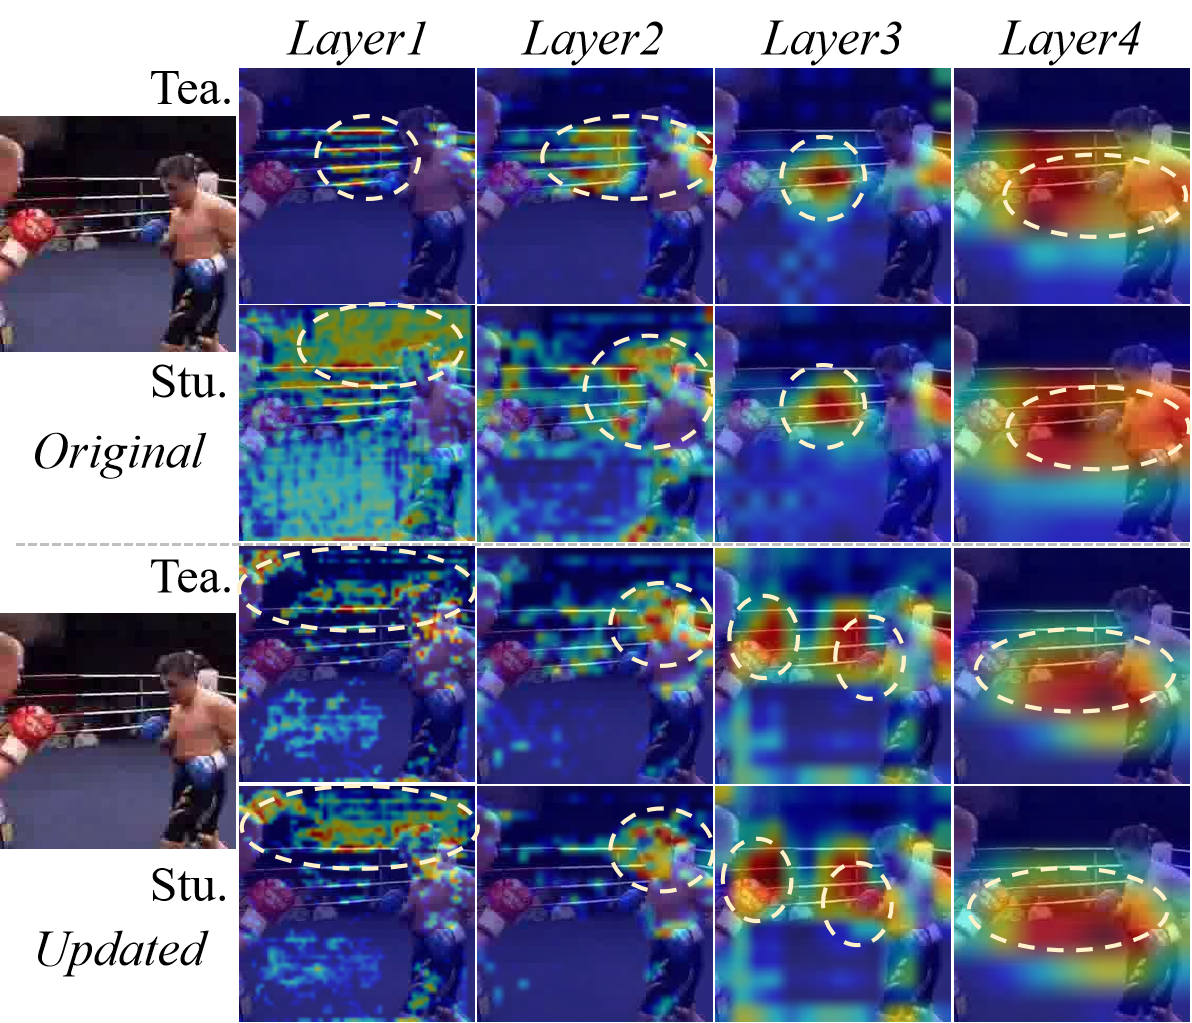
\includegraphics[width=0.49\textwidth]{pic/UCF101-vis1.png}
    \hfill 
    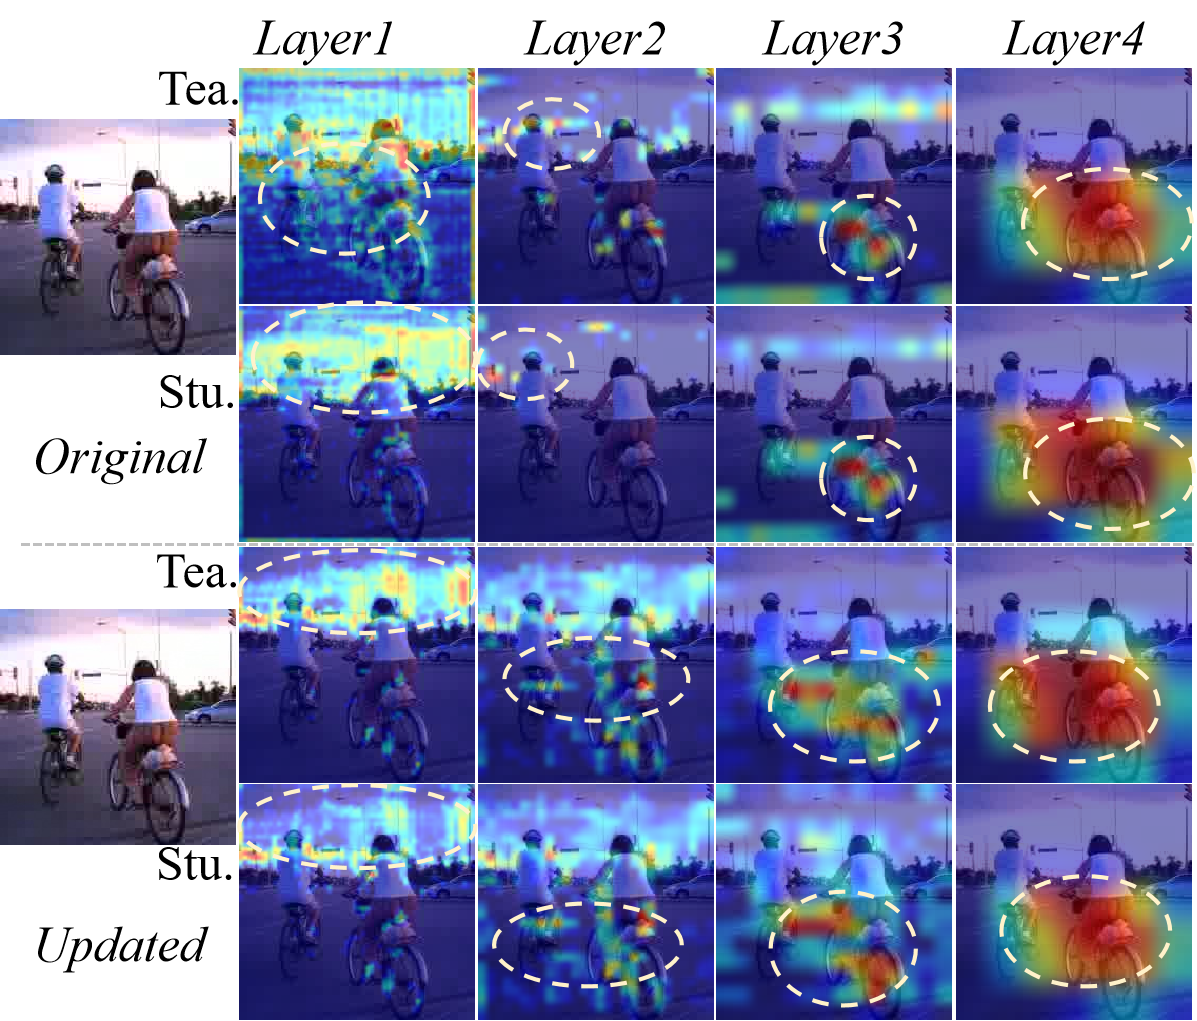
\includegraphics[width=0.49\textwidth]{pic/UCF101-vis2.png}
    \caption{UCF101\cite{soomro-arxiv2012-ucf101}数据集原始图像与生成图像上CAM\cite{zhou-cvpr2016-ldf}可视化图}
    \label{fig:ucf101}
\end{figure}

在UCF101数据集上，不难发现在模型浅层（Layer1、Layer2）更关注于背景，图\ref{fig:ucf101}的左图，教师模型更关注于拳击场的围栏，而学生模型还着重关注了拳击场的地面，当使用本文提出的方法后，学生模型的注意力会从地面逐步向围栏过渡，而教师模型不光会关注围栏部分也会逐步会向拳击地面（图中红圈所示），教师与学生的关注区域会趋向一致；右图的浅层模型也是同理，原始输入的教师模型关注于右侧的骑行者，而学生模型则更多的关注到背景，通过本文方法更新样本后，教师与学生的关注区域会趋向一致，教师与学生模型的关注区域都会趋向一致， 均会关注于背景知识或学生的骑行动作（图中红圈所示），当模型在深层（Layer3、Layer4）时，教师与学生模型均会逐渐关注与动作本身，但左图layer3时，教师与学生模型的专注点仍在拳击场的拦网处，使用本文提出的方法后，教师与学生模型的中间特征会关注于拳击运动员的手部，(黄圈所示)，在右图的layer3时，虽然原始的教师与学生模型关注到了右侧一个人的骑行动作，然而忽略了左侧运动员的骑行动作，这点在应用了本文更新后的训练样本后得到了极大的改善。

\begin{figure}[htbp]
    \centering
    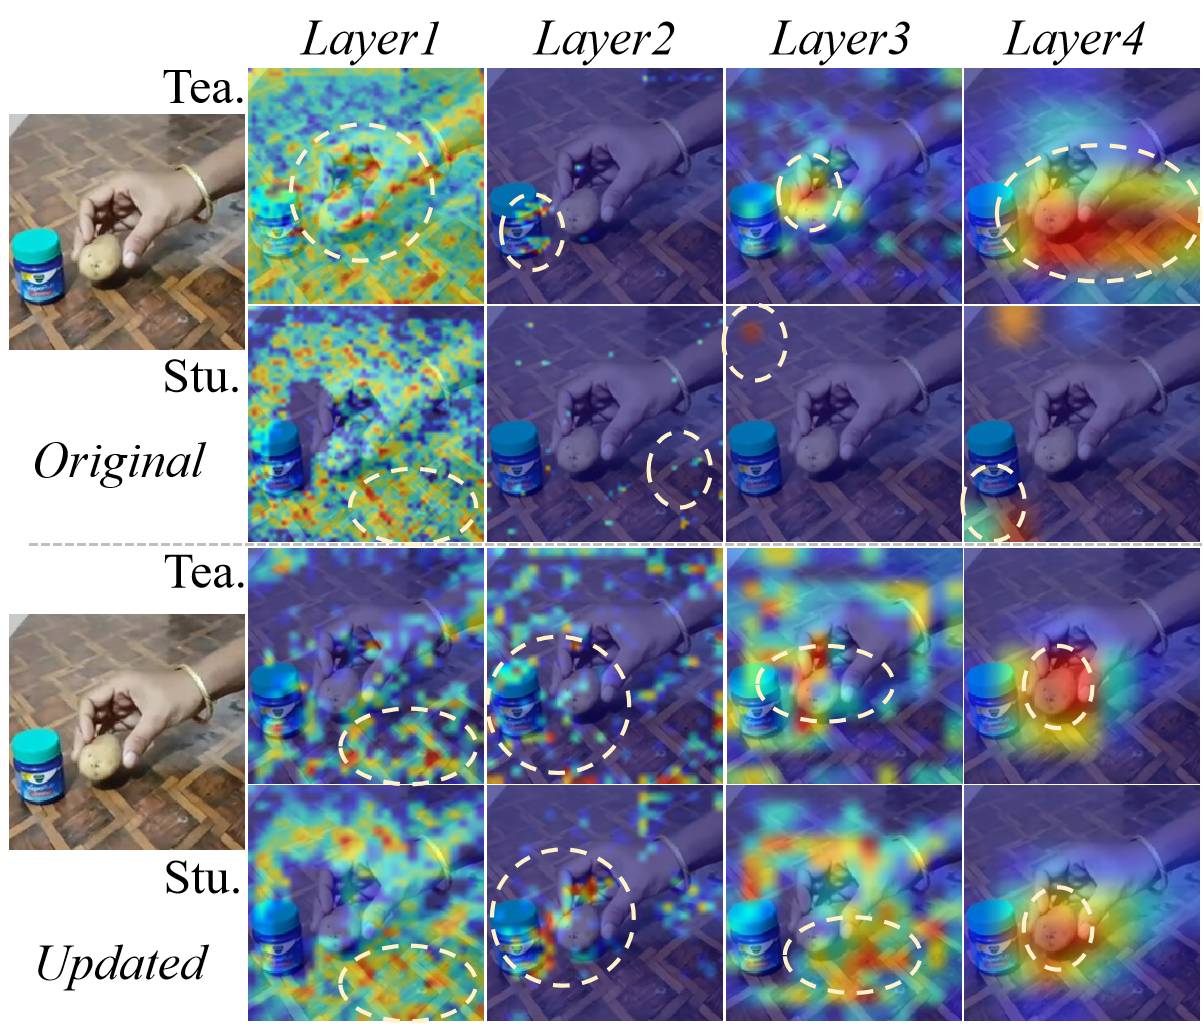
\includegraphics[width=0.49\textwidth]{pic/Sth-vis1.png}
    \hfill 
    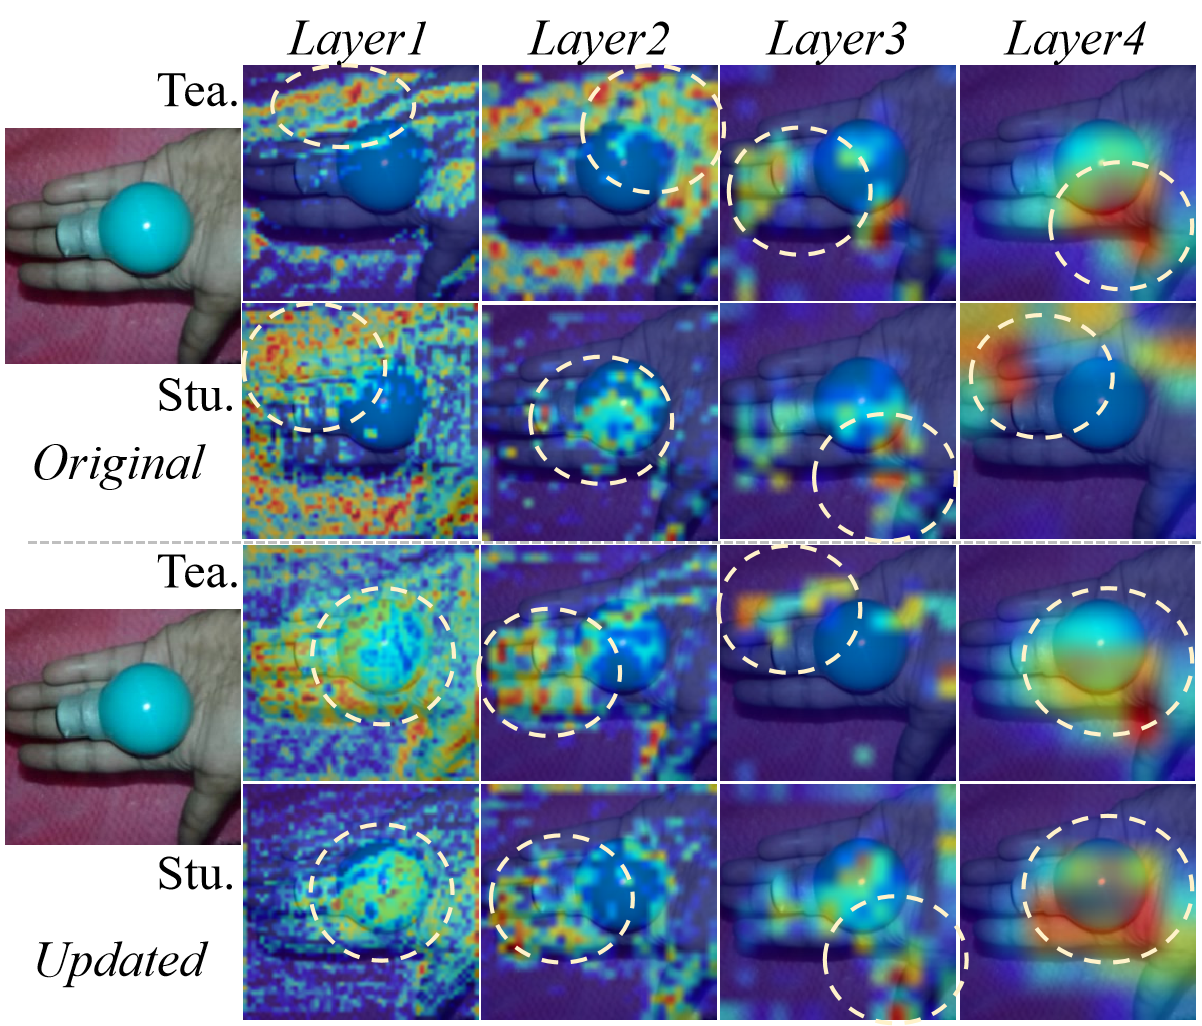
\includegraphics[width=0.49\textwidth]{pic/Sth-vis2.png}
    \caption{Sth-Sth v2\cite{goyal-iccv2017-sthsth}数据集原始图像与生成图像上CAM可视化图}
    \label{fig:Sth}
\end{figure}
在Sth-Sth数据集上，由于模型本身的准确并不高，可视化结果相较于UCF101数据集上并不明显，但无论是左图还是右图，使用更新后样本作为输入的浅层特征（Layer1、Layer2）热力图更聚焦于动作/物体本身（图中白圈所示），且教师与学生关注的区域会趋向一致；当模型在深层（Layer3、Layer4）时，教师与学生模型均会逐渐关注与动作本身，以左图为例，Layer4的热力图显示，以原始视频样本作为输入的教师模型虽然关注到了手与物体，但同时也关注了部分背景，而学生模型则关注区域完全偏移了，其冗余的信息无疑会增大学生模型学习难度；使用本文方法更新后的训练样本输入教师与学生模型后，教师与学生的关注区域均极其相似（黄圈所示），证明了本方法的有效性。

\begin{figure}[htbp]
    \centering
    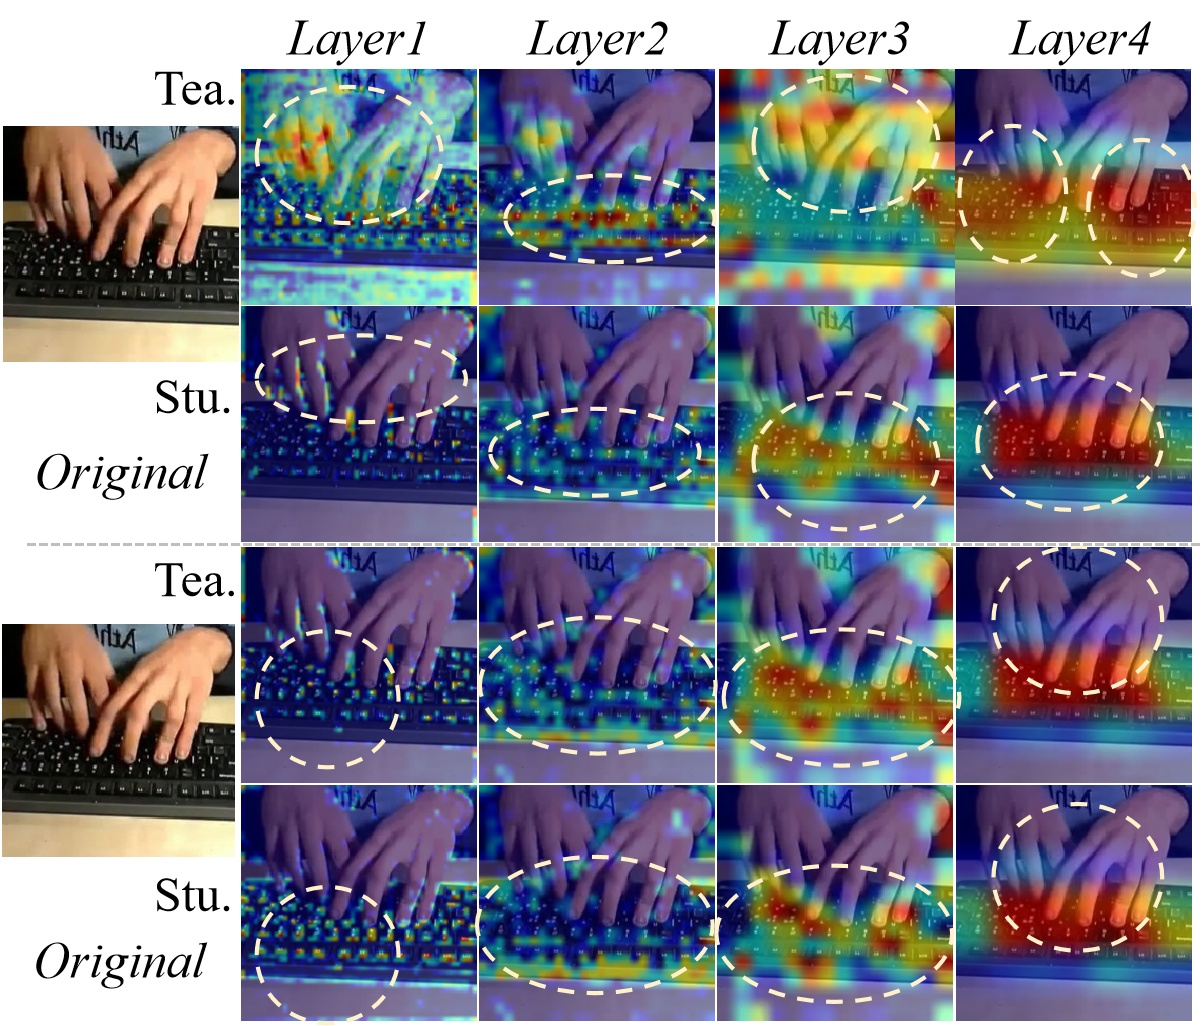
\includegraphics[width=0.49\textwidth]{pic/K400-vis1.png}
    \hfill 
    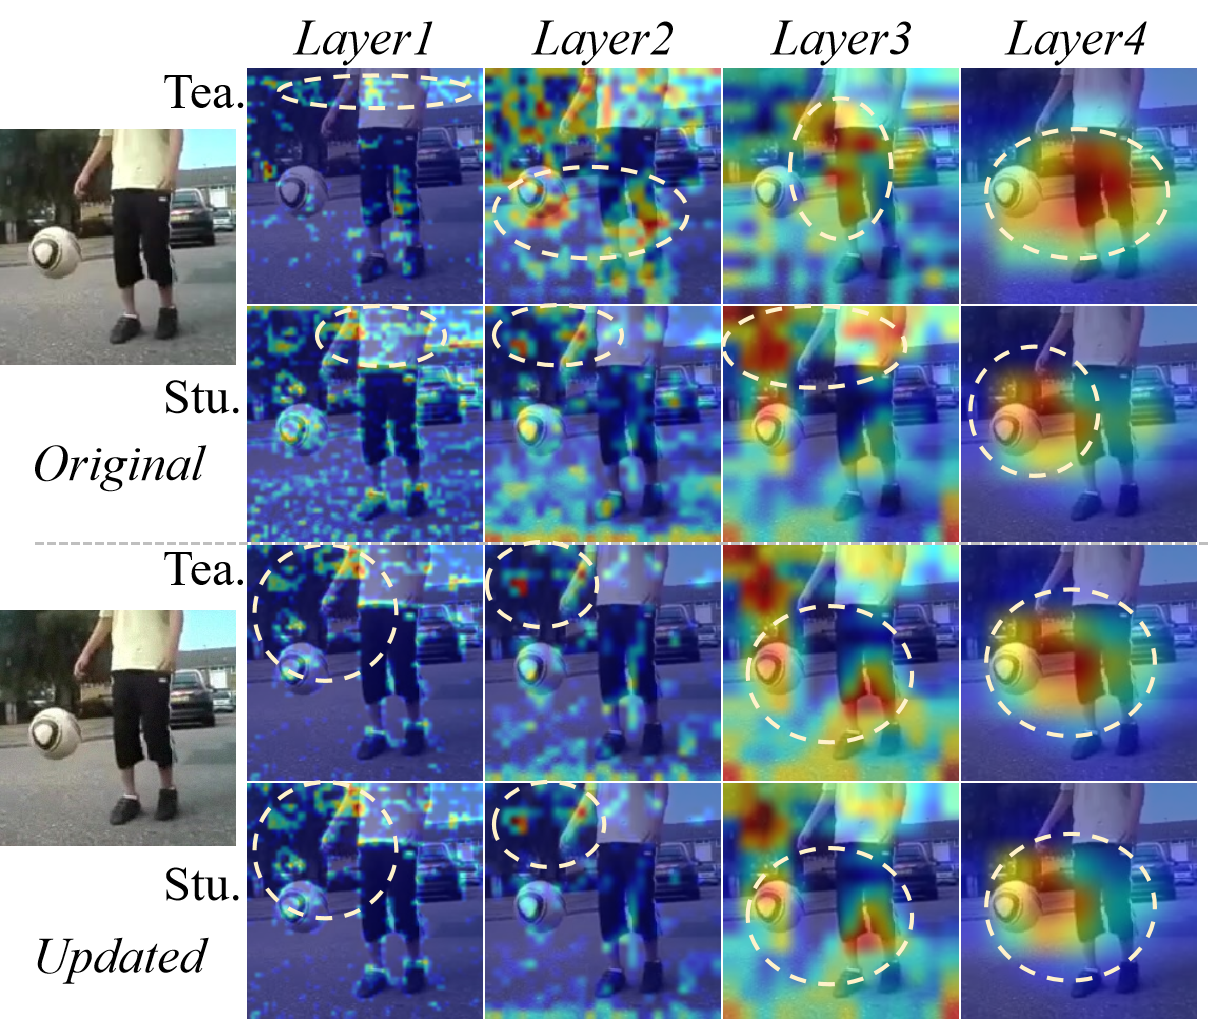
\includegraphics[width=0.49\textwidth]{pic/K400-vis2.png}
    \caption{Kinetics-400\cite{kay-arXiv2017-kinetics}数据集原始图像与生成图像上CAM可视化图}
    \label{fig:k400}
\end{figure}
在Kinetics-400数据集上，与UCF101数据集类似模型浅层更关注于背景知识，而深层更关注于动作本身，以左图为例，在原始视频输入的情况下，Layer1的教师模型准确的关注了手敲击键盘这一动作，但学生模型与教师模型的关注区域差别巨大，学生模型很难从教师模型中学到有用的知识，然而使用本文更新后的训练样本时，虽然教师模型关注的区域缩小了，但与学生模型关注的区域高度吻合（图中白圈所示），到模型深层次时，也是同理，在原始视频输入的情况下,虽然教师模型的关注度范围更大（覆盖到几乎所有键盘，但与学生模型的关注区域差异巨大）,而使用了本文方法更新后的训练样本时，教师与学生模型关注的区域高度一致（黄圈所示），证明了本方法的有效性。

\subsection{Channel fig}
\begin{figure}[!h]
    \centering
    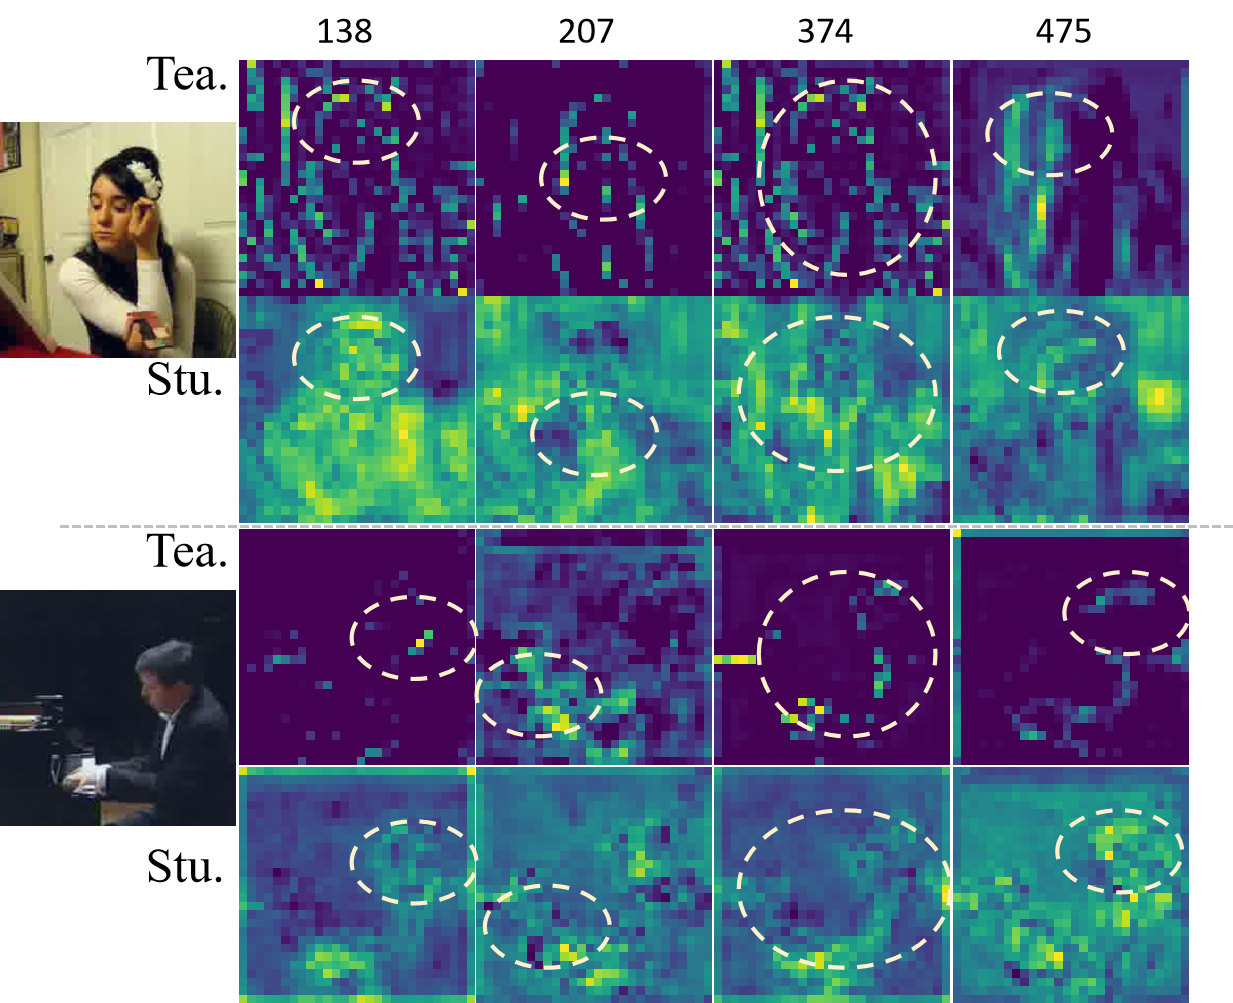
\includegraphics[width=0.48\textwidth]{pic/chanel-ucf.png}
    \caption{The Channel fig on the UCF101 Dataset \cite{soomro-arxiv2012-ucf101}}
    \label{fig:ucf-channel}
\end{figure}
如图所示为SlowFast模型在UCF101数据集上第二层Top-4通道的特征图可视化结果。可以看出，不同通道所提取的特征具有明显差异。具体而言，207通道在教师模型和学生模型中均显著关注动作相关特征（例如“Apply Eye Makeup”和“Playing Piano”中手部动作）；374通道则对执行动作的人物整体具有较强响应；而138通道除动作主体外，还保留了一定程度的背景信息，呈现出与其他通道不同的注意力分布

\begin{figure}[!h]
    \centering
    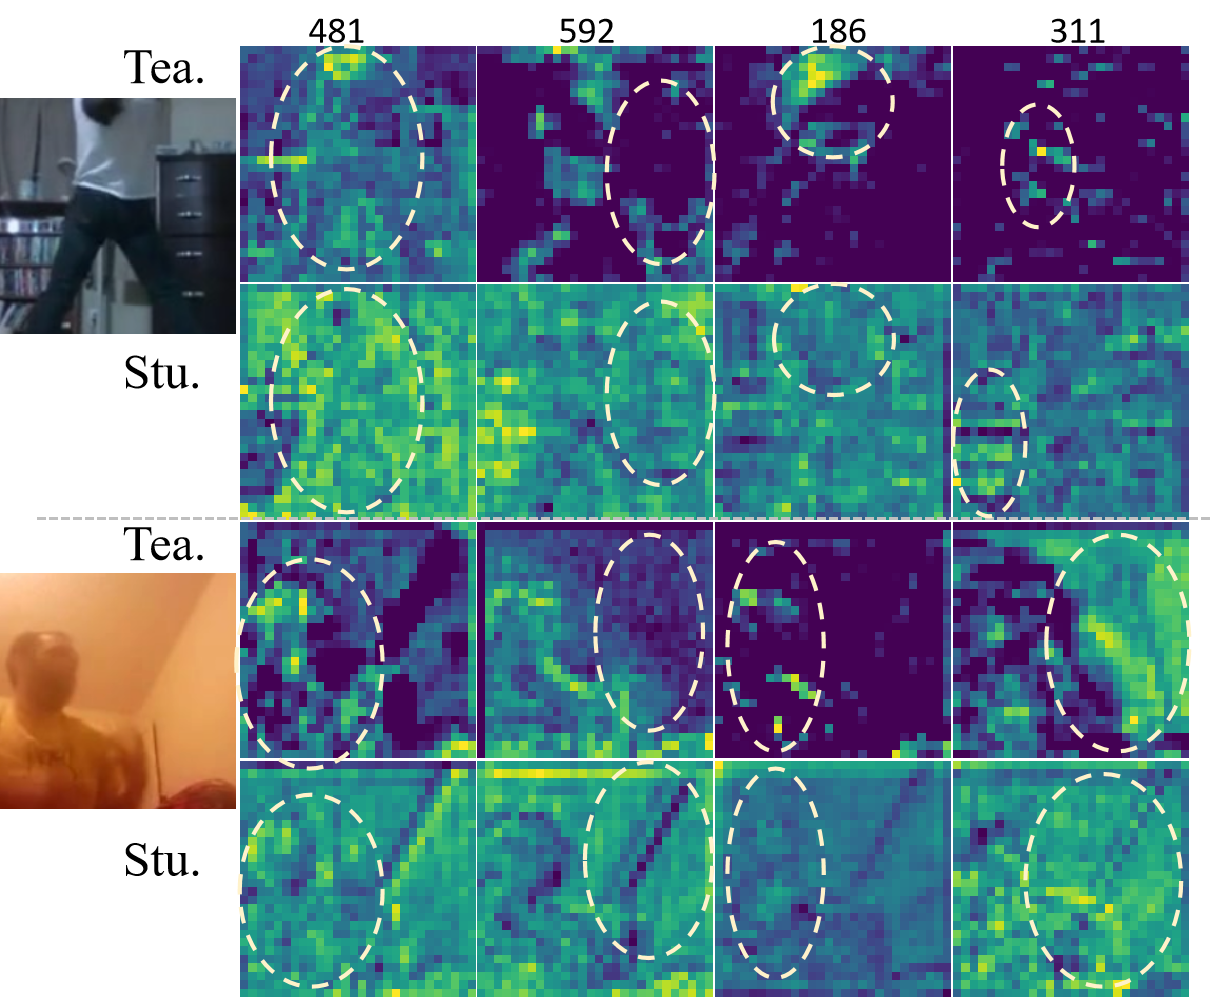
\includegraphics[width=0.48\textwidth]{pic/k400-channel.png}
    \caption{The Channel feature on the k400 Dataset \cite{kay-arXiv2017-kinetics}}
    \label{fig:k400-channel}
\end{figure}
如图所示为SlowFast模型在Kinetics数据集上第二层Top-4通道的特征图可视化结果。可以观察到，不同通道在特征响应上表现出明显差异。具体而言，481通道在教师模型和学生模型中均主要关注运动主体，同时对背景（如下方图像中墙面的边缘）也保持一定的响应；而311通道则更多聚焦于背景信息，如上图中书柜的纹理细节以及下图中边缘背景的结构特征，均在该通道中被显著刻画。上方bending back下方 contact juggling

\begin{figure}[!h]
    \centering
    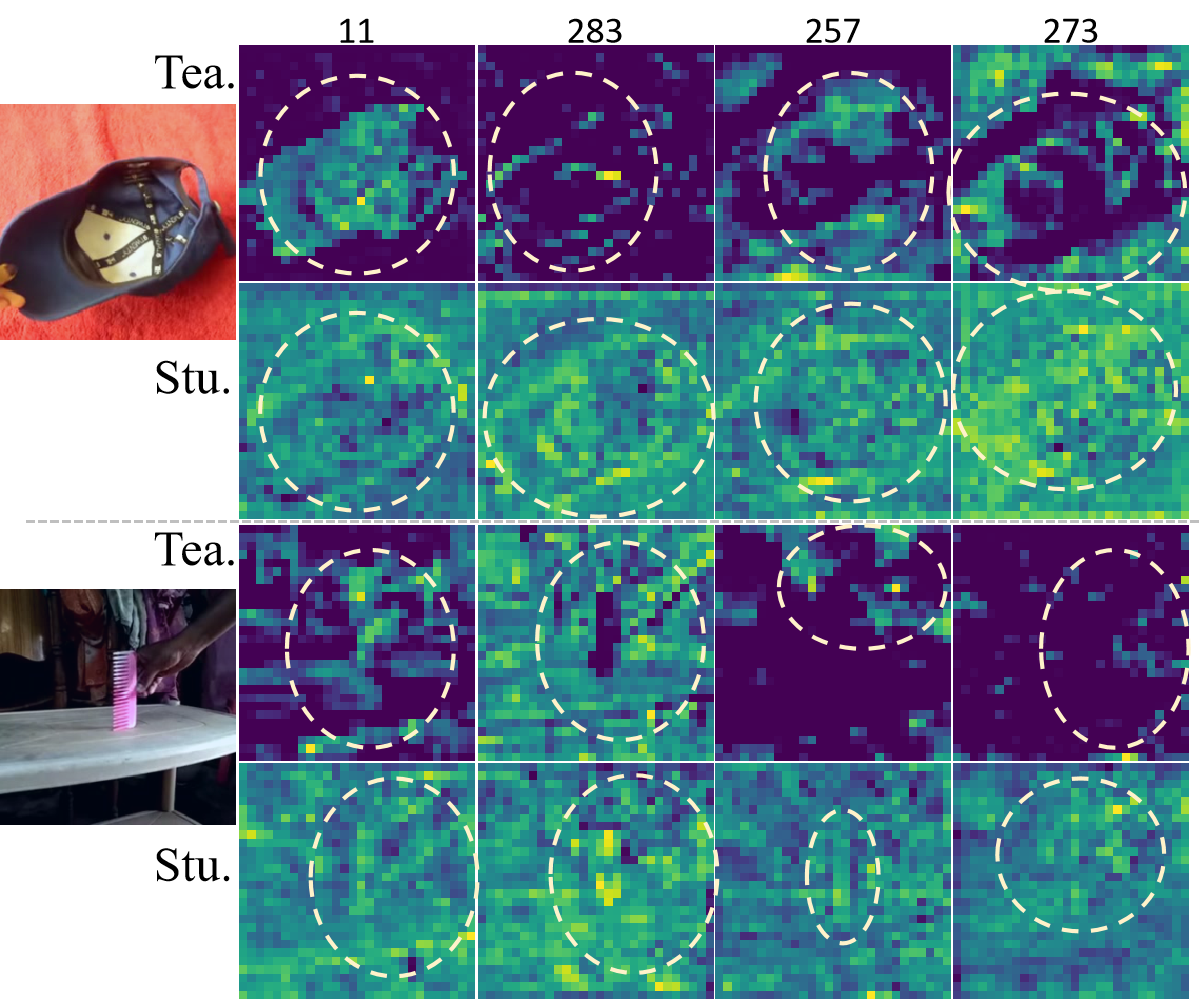
\includegraphics[width=0.48\textwidth]{pic/sth-channel.png}
    \caption{The Channel feature on the sth-sth-v2 Dataset \cite{goyal-iccv2017-sthsth}}
    \label{fig:sth-channel}
\end{figure}
如图所示为SlowFast模型在Something-Something-v2数据集上第二层Top-4通道的特征图可视化结果。分析可知，不同通道在特征响应模式上表现出显著差异。具体而言，11通道主要聚焦于图像中的核心动作目标，例如上图中的“帽子”与下图中“梳子”这类关键物体；而283通道则更倾向于提取物体的轮廓与边界信息，体现出对物体结构特征的敏感性。各通道通过不同的响应模式共同构建了对视频内容的多样的刻画48 Pretending to turn something upside down without actually turning it82 Folding something with one's hands



\subsection{Failure Case}
\begin{figure}[!h]
    \centering
    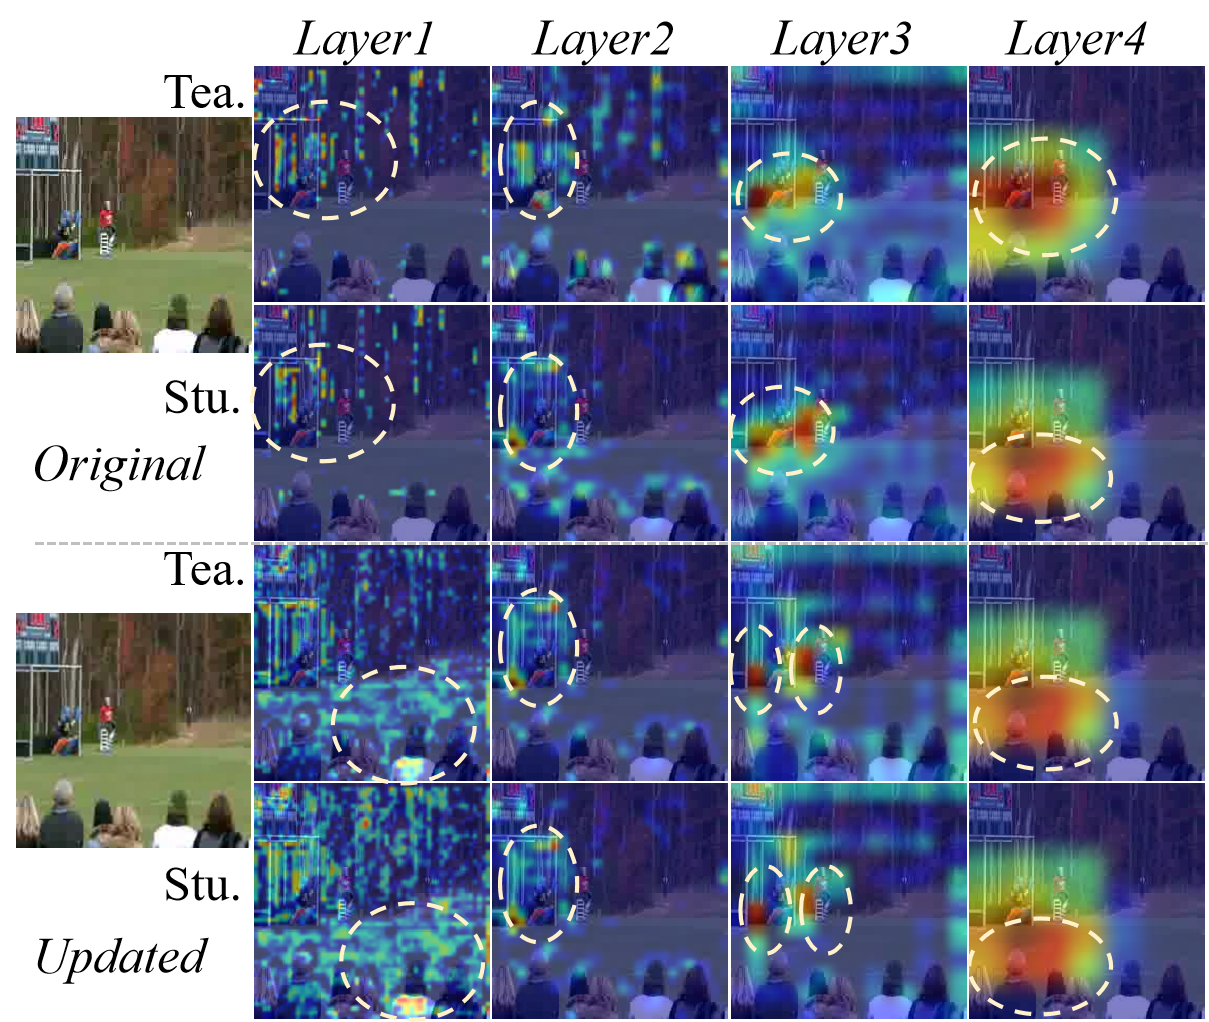
\includegraphics[width=0.48\textwidth]{pic/ucf-fail.png}
    \caption{The failure case on the UCF101 Dataset \cite{soomro-arxiv2012-ucf101}}
    \label{fig:ucf-fail}
\end{figure}
 UCF101   FieldHockeyPenalty  在曲棍球投掷动作的失败案例中，当场边存在大量观众等强干扰背景时，学生模型在浅层（Layer1）和深层（Layer4）特征中均表现出明显的注意力偏移，倾向于关注背景观众而非动作主体。尽管我们引入了频域对齐的样本更新策略以强化关键频率成分，并采用通道级自适应蒸馏来提升语义一致性，但背景区域本身包含丰富的中高频纹理，其频率分布与人体动作边缘高度重叠，使得频域对齐过程中部分背景成分被误识为“可学习结构”。

\begin{figure}[!h]
    \centering
    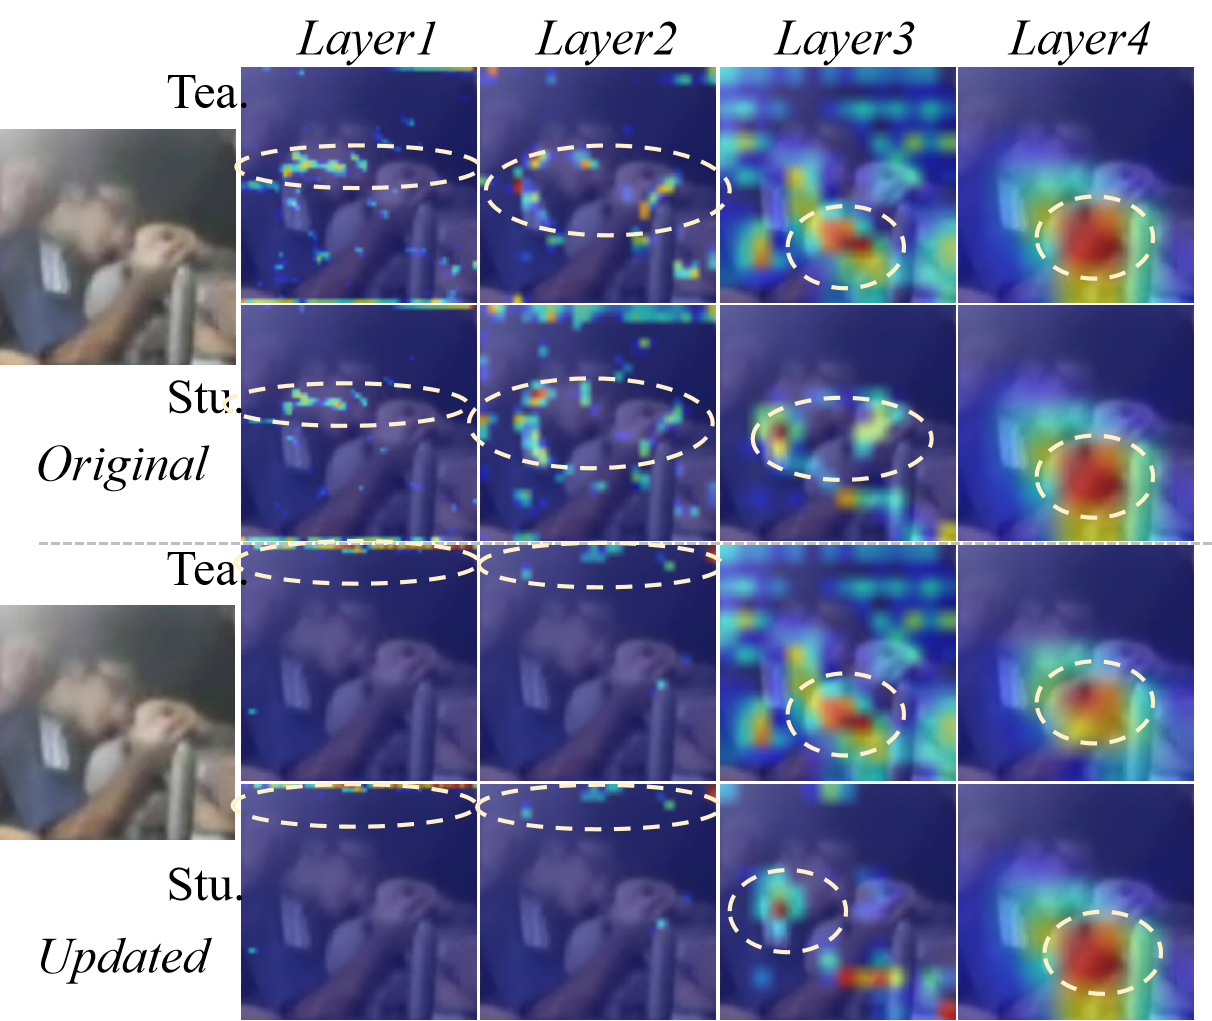
\includegraphics[width=0.48\textwidth]{pic/k400-fail.png}
    \caption{The failure case on the k400 Dataset \cite{kay-arXiv2017-kinetics}}
    \label{fig:k400-fail}
\end{figure}

Arm wrestling  Kinetics-400  在扳手腕这一动作场景中，由于双方长时间处于僵持状态，整体动作幅度较小且时序变化不明显，导致本文提出的 ASG 模块与 CDD 模块在时间维度上难以提取到具有判别性的频率变化信号。受此影响，教师模型与学生模型在中间特征层面的对齐效果受到显著削弱，从而影响最终的蒸馏性能
\begin{figure}[!h]
    \centering
    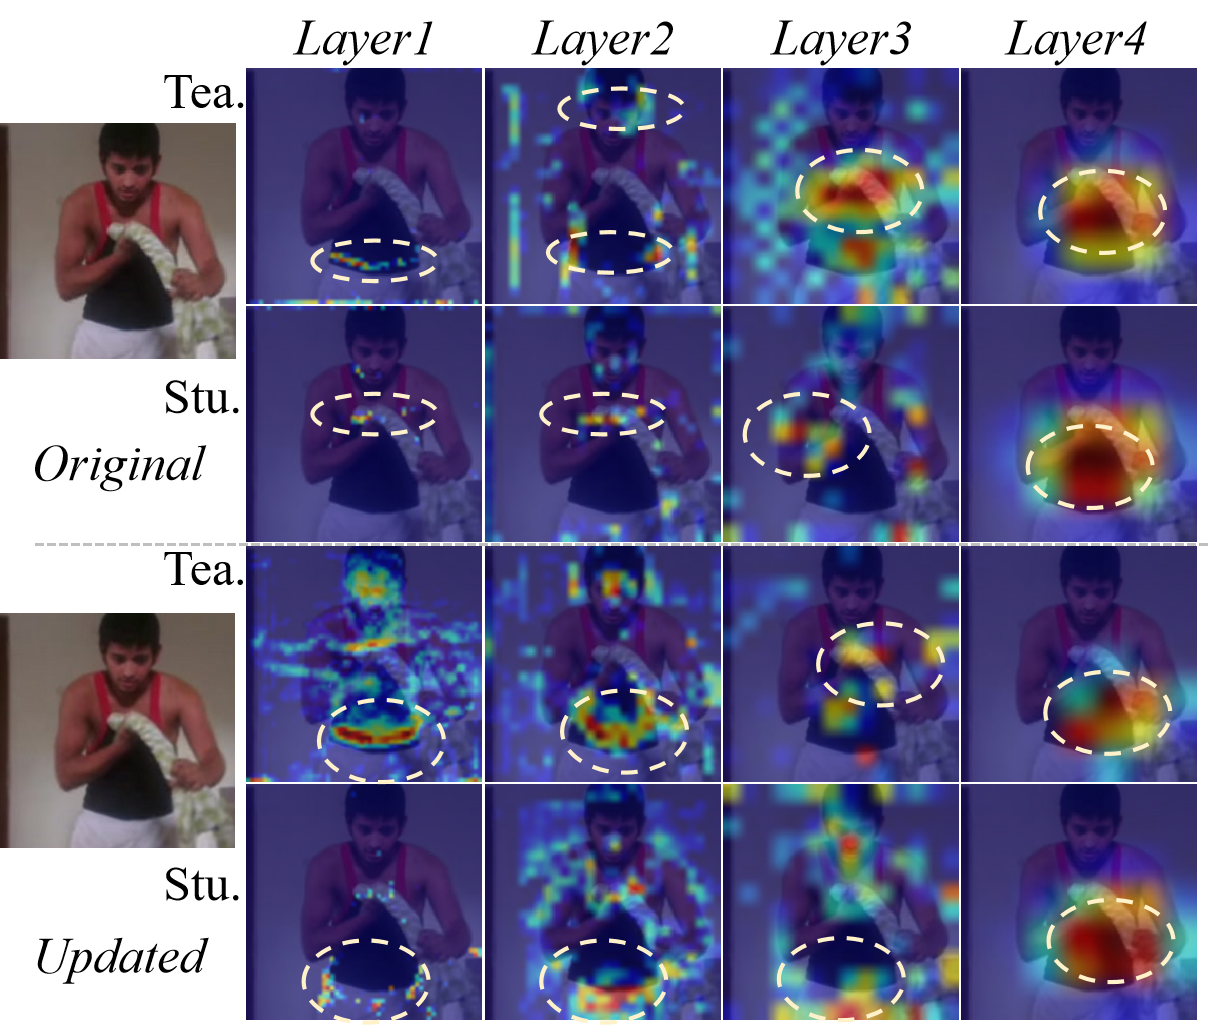
\includegraphics[width=0.48\textwidth]{pic/sth-fail.png}
    \caption{The failure case on the sth-sth-v2 Dataset \cite{goyal-iccv2017-sthsth}}
    \label{fig:sth-fail}
\end{figure}

Sth-sth  Wring towel  这一动作相对简单，且场景背景干扰较弱，使得在应用本方法前后，模型的特征分布整体变化并不显著。在此类低复杂度动作中，动作模式单一且时序结构相对稳定，ASG 与 CDD 等模块难以带来明显收益，反而引入了额外的时间开销，从而降低了整体的优化效率。
\subsection{关于损失上下界分析以及可视化}

为了证明式子\ref{eq:feat}的收敛性，本部分在UCF101\cite{soomro-arxiv2012-ucf101}数据集上绘制了式子中各部分的值，随epoch变化的曲线如图\ref{fig:curve}所示，可以看到中间特征部分由于与在实际蒸馏过程中的$\mathcal{L}_{feat}$方向一致，因此收敛的速度极快，而中心频率由于在训练初期是通过凯明初始化，可能在前一两次更新时其值可能会略微变大，如右上图的Layer2曲线，但各层的整体曲线均不断减小趋向收敛，教师与学生的中心频率会趋向于一致，教师模型与学生模型的中间特征的mse损失与中心频率的mse损失之比也最终趋向于收敛，可以发现Layer4的收敛速度相较于其他层收敛的更快。

\begin{figure}[!h]
    \centering
    \includegraphics[width=1\textwidth]{pic/Curve.png}
    \caption{UCF101\cite{kay-arXiv2017-kinetics}数据集各层教师与学生模型差异评估曲线}
    \label{fig:curve}
\end{figure}



关于下式：
\begin{equation}
\mathcal{L}^{c} = \frac{1}{N} \sum_{i=1}^{N} \sum_{l=1}^{L} \sum_{c=1}^{C_l^T} \frac{\left\| \bar{\textbf{F}}^{\mathcal{T}}_{i,l,c} - \bar{\textbf{F}}^{\mathcal{S}}_{i,l,c} \right\|_2^2}{\left\| \text{LN}(\omega_{l,c}^\mathcal{T})- \text{LN}(\omega_{l,c}^\mathcal{S}) \right\|_2^2+\epsilon}
\label{eq:align}
\end{equation}

由于输入视频片段$\textbf{X}_i$ 的像素值归一化到[-1,1],因此教师与学生模型的中间特征值$\bar{\textbf{F}}^{\mathcal{T}}_i$、$\bar{\textbf{F}}^{\mathcal{S}}_i$有界，且傅里叶变换和逆变换均为能量守恒操作（Parseval 定理）,因此滤波后特征存在上界$M$满足：

\begin{equation}
\left\| \bar{\textbf{F}}^{\mathcal{T}}_{i,l,c}(t,h,w)\right\|_1\leq M,
\left\|\bar{\textbf{F}}^{\mathcal{S}}_{i,l,c}(t,h,w)\right\|_1\leq M，
\end{equation}
其中$M$为特征值的最大值，最坏情况为两特征值符号相反时，

\begin{equation}
 \left| \bar{\textbf{F}}_{l,c}^\mathcal{T}(t,h,w) - \bar{\textbf{F}}_{l,c}^\mathcal{S}(t,h,w) \right|_2^2\leq (2M)^2=4M^2,
\end{equation}
将式\ref{eq:align}的分子部分按时空位置展开，则 ：
\begin{equation}
\left\| \bar{\textbf{F}}_{l,c}^\mathcal{T} - \bar{\textbf{F}}_{l,c}^\mathcal{S} \right\|_2^2 = 
\sum_{t=1}^{T_l} \sum_{h=1}^{H_l} \sum_{w=1}^{W_l} 
\left( \bar{\textbf{F}}_{l,c}^\mathcal{T}(t,h,w) - \bar{\textbf{F}}^\mathcal{S}(t,h,w) \right)^2\leq 4M^2T_lH_lW_l,
\label{eq:euclidean_expansion}
\end{equation}
在此基础上对于每一层中间特征,需要将各通道的中间特征进行累加：
\begin{equation}
\sum_{c=1}^{C_l^T} \left\| \bar{\textbf{F}}_{l,c}^\mathcal{T} - \bar{\textbf{F}}_{l,c}^\mathcal{S} \right\|_2^2 \leq 
4M^2 \sum_{c=1}^{C_l^T} T_l H_l W_l = 
4M^2 C_l^T T_l H_l W_l
\label{eq:channel_extension}
\end{equation}
对于分母部分，由于进行了Sigmoid 归一化$\text{LN}(\omega_{l,c}^\mathcal{S})\in[0,1]$,因此$\left\| \text{LN}(\omega_{l,c}^\mathcal{T}), \text{LN}(\omega_{l,c}^\mathcal{S}) \right\|_2^2+\epsilon\in[\epsilon,1+\epsilon]$,因此整个式子的上下界为：
\begin{equation}
\mathcal{L}^{c} \leq  \frac{1}{N} \sum_{i=1}^{N} \sum_{l=1}^{L} \frac{C_l^T \cdot 4M^2 T_l^\mathcal{T} H_l^\mathcal{T} W_l^\mathcal{T}}{\epsilon}
\end{equation}
\begin{equation}
\mathcal{L}^{c} \geq \frac{1}{N} \sum_{i=1}^{N} \sum_{l=1}^{L} \frac{1}{1+\epsilon} \sum_{c=1}^{C_l^T} \left\| \bar{\textbf{F}}_{i,l,c}^\mathcal{T} - \bar{\textbf{F}}_{i,l,c}^\mathcal{S} \right\|_2^2 \geq 0
\end{equation}


\section{Conclusion}
 
 本研究针对动作识别模型蒸馏任务，提出了频域自适应蒸馏方法，针对如何选择在学生模型当前学习阶段最适合其吸收知识的最佳教师模型等问题，设计了蒸馏自适应样本生成模块，首先通过设计可学习的频域高斯掩码动态提取判别性频带，实现特征空间的频域对齐；进一步引入梯度记忆机制，构建类别级代表性梯度方向，引导训练样本分布向更有利于知识迁移的方向优化，最终实现适配当前蒸馏阶段的动态增强训练集生成，从而显著提升蒸馏过程中的特征对齐效果；针对教师和学生的网络结构差异导致的中间特征差异使得两者难以静态对齐问题，提出通道级动态蒸馏模块，在蒸馏过程中，将更新后的视频输入分别送入教师与学生模型，提取多层中间特征和最终输出，通过1×1卷积实现特征对齐，并引入通道感知的频率对齐机制，引导学生模型在频域中逐通道对齐教师的语义表示。同时，结合类梯度记忆库构建的类间相似性分布，对学生模型的输出Logits施加软约束，使其更好地捕捉全局类别结构。在未来的工作中，可以在更复杂的视觉任务，如时空动作检测、目标检测中证明方法的有效性。
\bibliography{work2}
\end{document}
